\documentclass[10pt]{article}

% Set letter paper size:
% \setlength{\paperheight}{11in}
% \setlength{\paperwidth}{8.5in}
\usepackage[left=2.5cm,right=2.5cm,top=2.8cm,bottom=2.8cm]{geometry}

\usepackage{amsmath}
\usepackage{booktabs}
\usepackage[caption=false]{subfig}
\usepackage{xifthen}
\usepackage{xspace}
\usepackage{listings}
\usepackage{enumitem}
\usepackage{bm} % bold symbols
\usepackage{array}
\usepackage{amssymb}
\usepackage{balance}
\usepackage{url}
\usepackage{anyfontsize}
\usepackage{multirow}
\usepackage{stmaryrd}
\SetSymbolFont{stmry}{bold}{U}{stmry}{m}{n}

\usepackage{hyperref}
\usepackage{pgfplots}
\pgfplotsset{compat=1.8}
\usetikzlibrary{decorations.pathreplacing,calligraphy,backgrounds}

% \usepackage{mdframed}
% \mdfdefinestyle{MyFrame}{
% %linecolor=blue,
% outerlinewidth=2pt,
% roundcorner=5pt,
% leftmargin=100pt,
% innertopmargin=\baselineskip,
% innerbottommargin=1pt,
% innerrightmargin=20pt,
% innerleftmargin=100pt,
% backgroundcolor=gray!30!white
% }


% % Temporary
% \usepackage{todonotes}

\usepackage{tikz} 
\usetikzlibrary{topaths,calc,shapes,decorations.pathmorphing,arrows}

\usepackage{amsmath,amsthm}
\definecolor{purple}{rgb}{1, 0, 1}

\newcommand{\ie}{\emph{i.e.,}\xspace}
\newcommand{\eg}{\emph{e.g.,}\xspace}
\newcommand{\abr}{\emph{abbr.}\xspace}
\newcommand{\ea}{\emph{et al.}\xspace}
\newcommand{\gensync}{\emph{GenSync}\xspace}
\newcommand{\colosseum}{\emph{Colosseum}\xspace}
\newcommand{\srep}{\emph{SREP}\xspace} % Set Reconciliation Enhances
\newcommand{\srepsim}{\emph{SREPSim}\xspace}
% Propagation
\newcommand{\esrep}{\emph{E-SREP}\xspace}
\newcommand{\epsrep}{\emph{EP-SREP}\xspace}
\newcommand{\mesrep}{\emph{ME-SREP}\xspace}
\newcommand{\mempoolsync}{\emph{MempoolSync}}

\newcommand{\fref}[1]{Fig.~\ref{#1}}
\newcommand{\tref}[1]{Table~\ref{#1}}
\newcommand{\aref}[1]{Algorithm~\ref{#1}}
\newcommand{\procref}[1]{Procedure~\ref{#1}}
\newcommand{\sref}[1]{Section~\ref{#1}}
\newcommand{\lineref}[1]{line~\ref{#1}}
\newcommand{\appref}[1]{Appendix~\ref{#1}}

% Change \eqref
\LetLtxMacro{\originaleqref}{\eqref}
\renewcommand{\eqref}{Eq.~\originaleqref}

% Theorems and corollaries
\newcounter{theoremcount}
\setcounter{theoremcount}{0}
\DeclareRobustCommand{\theorem}[1]{%
  \refstepcounter{theoremcount}%
  \noindent\textit{\textbf{Theorem \thetheoremcount\label{theorem:#1}: }}%
}
\DeclareRobustCommand{\theoremref}[1]{Theorem~\ref{theorem:#1}}

\DeclareRobustCommand{\proof}{\emph{Proof:}\xspace}
\DeclareRobustCommand{\qqed}{\hfill$\blacksquare$}

\newcounter{corollcount}
\setcounter{corollcount}{0}
\DeclareRobustCommand{\coroll}[1]{%
  \refstepcounter{corollcount}%
  \noindent\textit{\textbf{Corollary \thecorollcount\label{coroll:#1}: }}%
}
\DeclareRobustCommand{\corollref}[1]{Corollary~\ref{coroll:#1}}

\newcounter{lemmacount}
\setcounter{lemmacount}{0}
\DeclareRobustCommand{\lemma}[1]{%
  \refstepcounter{lemmacount}%
  \noindent\textit{\textbf{Lemma \thelemmacount\label{lemma:#1}: }}%
}
\DeclareRobustCommand{\lemmaref}[1]{Lemma~\ref{lemma:#1}}

\newcounter{definitioncount}
\setcounter{definitioncount}{0}
\DeclareRobustCommand{\definition}[1]{%
  \refstepcounter{definitioncount}%
  \noindent\textit{\textbf{Definition \thedefinitioncount\label{definition:#1}: }}%
}
\DeclareRobustCommand{\defref}[1]{Definition~\ref{definition:#1}}

%notes of different authors
\newif\ifnotes
\notestrue
\notesfalse

\newif\ifdiff
\difftrue
\difffalse

\newcommand{\anote}[1]{\ifnotes $\ll$\textsf{\textcolor{purple}{Ari: {#1}}}$\gg$ \fi}
\newcommand{\nnote}[1]{\ifnotes $\ll$\textsf{\textcolor{orange}{Novak: {#1}}}$\gg$ \fi}
\newcommand{\diff}[1]{\ifdiff\textcolor{orange}{#1}\else#1\fi}

%%% Local Variables:
%%% mode: latex
%%% TeX-master: "main"
%%% End:


\title{F-IVM: Analytics over Relational Databases under Updates}

\author{Ahmet Kara \and Milos Nikolic \and Dan Olteanu \and Haozhe Zhang}


\author{
Ahmet Kara$^2$, 
Milos Nikolic$^1$, 
Dan Olteanu$^2$, 
Haozhe Zhang$^2$ 
\\ \\
$^1$University of Edinburgh
\enspace\enspace 
$^2$University of Zurich  
}
\date{}
% The correct dates will be entered by the editor

\begin{document}

\maketitle 
\begin{abstract}
    This article describes F-IVM,  a unified approach for maintaining analytics over changing relational data. We exemplify its versatility in four disciplines: processing queries with group-by aggregates and joins; learning linear regression models using the covariance matrix of the input features; building Chow-Liu trees using pairwise mutual information of the input features; and matrix chain multiplication. 

    F-IVM has three main ingredients: higher-order incremental view maintenance; factorized computation; and ring abstraction. F-IVM reduces the maintenance of a task to that of a hierarchy of simple views. Such views are functions mapping keys, which are tuples of input values, to payloads, which are elements from a ring. F-IVM also supports efficient factorized computation over keys, payloads, and updates. Finally, F-IVM treats uniformly seemingly disparate tasks. In the key space, all tasks require joins and variable marginalization. In the payload space, tasks differ in the definition of the sum and product ring operations.
 
    We implemented F-IVM on top of DBToaster and show that it can outperform classical first-order and fully recursive higher-order incremental view maintenance by orders of magnitude while using less memory.
\end{abstract}


\paragraph{Acknowledgements}
This project has received funding from the European Union's Horizon 2020 research and innovation programme under grant agreement No 682588.


\section{Introduction}
\label{sec:introduction}
% \begin{itemize}
%     % Diffusion of FL
%     \item {\st{Diffusion of FL}}
%     % Security threats to FL
%     \item {\st{Security threats to FL with particular focus on model poisoning}}
%     % Limitations of existing countermeasures
%     \item {\st{Current countermeasures (e.g., KRUM) and their limitations}}
%     % Proposed method and its advantages
%     \item {\st{Intuitive description of the proposed method and its difference (i.e., advantages) w.r.t. state of the art}}
%     % Main contributions
%     \item {\st{Summary of the main contributions of this work}}
%     % Paper's structure and organization
%     \item {\st{Paper's structure and organization}}
% \end{itemize}

% Diffusion of FL
Recently, {\em federated learning} (FL) has emerged as the leading paradigm for training distributed, large-scale, and privacy-preserving machine learning (ML) systems~\cite{mcmahan2017googleai,mcmahan2017aistats}. 
The core idea of FL is to allow multiple edge clients to collaboratively train a shared, global model without disclosing their local private training data.
%Specifically, an FL system consists of a central server and many edge clients; 
A typical FL round involves the following steps: {\em(i)} the server randomly picks some clients and sends them the current, global model; {\em(ii)} each selected client locally trains its model with its own private data; then, it sends the resulting local model to the server;\footnote{Whenever we refer to global/local model, we mean global/local model {\em parameters}.} {\em(iii)} the server updates the global model by computing an \emph{aggregation function}, usually the average (FedAvg), on the local models received from clients.
% \begin{enumerate}
%     \item[{\em(i)}] the server sends the current, global model to the clients and appoints some of them for training;
%     \item[{\em(ii)}] each selected client locally trains its copy of the global model with its own private data; then, it sends the resulting local model back to the server;\footnote{Whenever we refer to global/local model, we mean global/local model {\em parameters}.}
%     \item[{\em(iii)}] the server updates the global model by computing an \emph{aggregation function} on the local models received from clients (by default, the average, also referred to as FedAvg~\cite{mcmahan2017aistats}).
% \end{enumerate}
This process goes on until the global model converges. %(e.g., after a certain number of rounds or other similar stopping criteria).
%\\
% The advantages of FL over the traditional, centralized learning paradigm are undoubtedly clear in terms of flexibility/scalability (clients can join/disconnect from the FL network dynamically), network communications (only model weights\footnote{We will use \textit{parameters} and \textit{weights} interchangeably.} are exchanged between clients and server), and privacy (each client's private training data is kept local at the client's end and not uploaded to the server).
\\
% Security threats to FL
%However, the growing adoption of FL also raises security concerns~\cite{costa2022covert}, particularly about its confidentiality, integrity, and availability.
Although its advantages over standard ML, FL also raises security concerns~\cite{costa2022covert}. %, particularly about its confidentiality, integrity, and availability~\cite{costa2022covert}.
% OLD, LONG VERSION
% Indeed, some work deals with privacy leakage that may expose the local data of some clients~\cite{melis2019sp}. 
% A large body of work, instead, investigates attacks that usually aim to detriment the predictive accuracy of the learned global model. For instance, \emph{data poisoning} attacks achieve this goal by letting an adversary pollute the training set of some corrupt FL clients with maliciously crafted examples~\cite{jagielski2018sp}.
% Similarly, in \emph{model poisoning} the attacker attempts to tweak the global model weights~\cite{bhagoji2019pmlr} by directly perturbing the local model's weights of some infected FL clients before these are sent to the central server for aggregation, usually via so-called Byzantine attacks. 
% It turns out that Byzantine model poisoning attacks severely impact standard FedAvg; therefore, more robust aggregation functions must be designed to make FL systems secure.
Here, we focus on \emph{untargeted model poisoning} attacks~\cite{bhagoji2019pmlr}, where an adversary attempts to tweak the global model weights %\footnote{We will use the terms \textit{parameters} and \textit{weights} interchangeably.} 
by directly perturbing the local model's parameters of some infected clients before these are sent to the central server for aggregation.
In doing so, the adversary aims to jeopardize the global model \textit{indiscriminately} at inference time.
Such model poisoning attacks severely impact standard FedAvg; therefore, more robust aggregation functions must be designed to secure FL systems.
\\
% In this paper, we focus on designing a novel robust aggregation scheme at the server's end to contrast the effect of Byzantine model poisoning attacks.
%
% Current countermeasures and their limitations
%Several countermeasures have been proposed in the literature to combat model poisoning attacks on FL systems.
% Some methods use simple statistics more robust than plain average to smooth the impact of malicious updates (e.g., Trimmed Mean and FedMedian~\cite{yin2018icml}). 
% Other defenses implement outlier detection techniques to discard malicious updates from the aggregation performed at the server's end. Those are either based on heuristics (e.g., Krum/Multi-Krum~\cite{blanchard2017nips} and Bulyan~\cite{mhamdi2018pmlr}) or data-driven approaches (e.g., K-means clustering~\cite{shen2016acm} or DnC via spectral analysis~\cite{shejwalkar2021ndss}). 
% Finally, some strategies rely on a centralized ``source of trust'' to spot potential malicious updates (e.g., FLTrust~\cite{cao2020fltrust}).
% Several countermeasures have been proposed in the literature to combat model poisoning attacks on FL systems, i.e., to discard possible malicious local updates from the aggregation performed at the server's end. 
% These techniques range from simple statistics more robust than plain average (e.g., Trimmed Mean and FedMedian~\cite{yin2018icml}) to outlier detection heuristics (e.g., Krum/Multi-Krum~\cite{blanchard2017nips} and Bulyan~\cite{mhamdi2018pmlr}) or data-driven approaches (e.g., spectral analysis via K-means clustering~\cite{shen2016acm} or spectral analysis), or methods based on ``source of trust'' (e.g., FLTrust~\cite{cao2020fltrust}).
% OLD, LONG VERSION
%Several countermeasures have been proposed in the literature to combat Byzantine model poisoning attacks on FL systems.
% Descriptive statistics
% For example, Trimmed Mean and FedMedian aggregate local model updates using more robust statistics than standard average~\cite{yin2018icml}.
%
% % Heuristics for outlier detection
% Many existing Byzantine-resilient strategies implement some outlier detection heuristics to discard the model updates sent by potentially malicious clients from the input of the aggregation function.
% One of the most popular heuristics is Krum~\cite{blanchard2017nips}.
% This strategy tries to mitigate the impact of Byzantine attacks by selecting as a global model the local model with the smallest sum of Euclidean distances to {\em all} the other local models.
% Although powerful, Krum requires the server to know (or, at least, estimate) the number of malicious FL clients upfront, which is generally impossible in a realistic attack scenario. %
% Moreover, Krum may become ineffective for complex, high-dimensional model parameter spaces due to the curse of dimensionality.
% Bulyan~\cite{mhamdi2018pmlr} tries to overcome this issue by combining Krum with a variant of Trimmed Mean.
% % Data-driven outlier detection
% Other strategies use data-driven outlier detection techniques -- e.g., via K-means clustering~\cite{shen2016acm} -- to spot potential malicious local model updates. 
% %For instance, Shen et al. propose to cluster local model updates with K-means and thus identify outliers.
%
% % Other techniques
% As far as the server is concerned, any local model received can be from a potential malicious client. 
% FLTrust~\cite{cao2020fltrust} assumes the server acts as a client, i.e., trains a local model on an additional {\em trustworthy} dataset at the server's end and compares it against all the local models from other clients. 
% This way, the server can rely on some ``source of trust'' when discarding potentially malicious clients.
%\\
% Limitations of existing Byzantine-resilient strategies
Unfortunately, existing defense mechanisms either rely on simple heuristics (e.g., Trimmed Mean and FedMedian by~\cite{yin2018icml}) or need strong and unrealistic assumptions to work effectively (e.g., foreknowledge or estimation of the number of malicious clients in the FL system, as for Krum/Multi-Krum~\cite{blanchard2017nips} and Bulyan~\cite{mhamdi2018pmlr}, which, however, cannot exceed a fixed threshold).
Furthermore, outlier detection methods using K-means clustering~\cite{shen2016acm} or spectral analysis like DnC~\cite{shejwalkar2021ndss} do not directly consider the temporal evolution of local model updates received.
Finally, strategies like FLTrust~\cite{cao2020fltrust} require the server to collect its own dataset and act as a proper client, thereby altering the standard FL protocol.
\\
% OLD, LONG VERSION
% Overall, existing Byzantine-resilient strategies are either simple heuristics (e.g., FedMedian) or, if they are more complex, they rely on strong and unrealistic assumptions to work effectively (e.g., knowing the number of malicious clients in the FL system in advance, as for Krum and alike).
% Furthermore, data-driven outlier detection methods do not consider the temporary evolution of local model updates received (e.g., K-means clustering). 
% Finally, strategies like FLTrust requires the server to collect its own dataset and act as a proper client, thereby altering the standard FL protocol.
%
% Description of the proposed method
This work introduces a novel pre-aggregation \textit{filter} robust to untargeted model poisoning attacks. Notably, this filter $(i)$ operates without requiring prior knowledge or constraints on the number of malicious clients and $(ii)$ inherently integrates temporal dependencies. 
The FL server can employ this filter as a preprocessing step before applying \textit{any} aggregation function, be it standard like FedAvg or robust like Krum or Bulyan.
Specifically, we formulate the problem of identifying corrupted updates as a multidimensional (i.e., matrix-valued) time series anomaly detection task. 
The key idea is that legitimate local updates, resulting from well-calibrated iterative procedures like stochastic gradient descent (SGD) with an appropriate learning rate, show \textit{higher predictability} compared to malicious updates. This hypothesis stems from the fact that the sequence of gradients (thus, model parameters) observed during legitimate training exhibit regular patterns, as validated in Section~\ref{subsec:intuition}. %until convergence. 
%This regularity may be more pronounced for smooth convex loss functions, but it can still be captured within an appropriate time window, even for more complex and convoluted loss surfaces. 
%We provide evidence of this claim in Appendix~B, where we show that the average mutual information (i.e., ``predictability''), calculated over pairs of legitimate model updates sent at different FL rounds, is significantly higher than the corresponding computation for a malicious client.
\\
Inspired by the matrix autoregressive (MAR) framework for multidimensional time series forecasting~\cite{chen2021je}, we propose the FLANDERS ({\em \textbf{F}ederated \textbf{L}earning meets \textbf{AN}omaly \textbf{DE}tection for a \textbf{R}obust and \textbf{S}ecure}) filter.
The main advantages of FLANDERS over existing strategies like FLDetector~\cite{zhao2020multivariate} are its resilience to large-scale attacks, where $50\%$ or more FL participants are hostile, and the capability of working under realistic non-iid scenarios.
We attribute such a capability to two key factors: $(i)$ FLANDERS works without knowing a priori the ratio of corrupted clients, and $(ii)$ it embodies temporal dependencies between intra- and inter-client updates, quickly recognizing local model drifts caused by evil players. Below, we summarize our main contributions:

\begin{itemize}
\item[{\em(i)}]
We provide empirical evidence that the sequence of models sent by legitimate clients is more predictable than those of malicious participants performing untargeted model poisoning attacks.
\\
\item[{\em(ii)}] 
We introduce FLANDERS, the first pre-aggregation filter for FL robust to untargeted model poisoning based on multidimensional time series anomaly detection.
\\
\item[{\em(iii)}] 
We integrate FLANDERS into Flower,\footnote{\scriptsize{\url{https://flower.dev/}}} a popular FL simulation framework for reproducibility.
\\
\item[{\em(iv)}] 
We show that FLANDERS improves the robustness of the existing aggregation methods under multiple settings: different datasets, client's data distribution (non-iid), models, and attack scenarios.
\\
\item[{\em(v)}] 
We publicly release all the implementation code of FLANDERS along with our experiments.\footnote{\scriptsize{\url{https://anonymous.4open.science/r/flanders_exp-7EEB}}}
\end{itemize}

% Paper's structure and organization
The remainder of the paper is structured as follows. %some related work and the current state-of-the-art solutions to security issues that FL entails. 
Section~\ref{sec:background} covers background and preliminaries. 
In Section~\ref{sec:related}, we discuss related work.
Section~\ref{sec:problem} and Section~\ref{sec:method} describe the problem formulation and the method proposed. % to tackle it. 
Section~\ref{sec:experiments} gathers experimental results. %, and Section~\ref{sec:limitations} discusses some limitations of this work.
Finally, we conclude in Section~\ref{sec:conclusion}.
 %discusses the limitations of this work and draws future research directions.
%reports conclusions and draws perspectives for future research directions.

%%%%%%% OLD %%%%%%%
%to overcome the resilience of Byzantine failures in distributed Stochastic Gradient Descent computations. 
% The strength of Krum is its time complexity, which is linear in the gradient dimension. 
% However, the robustness of the approach is guaranteed for gradient-based learning applications only when the majority of the clients are not compromised. 
% Besides, the aggregation mechanism of Krum, as well as that of similar methods, is robust from a coarse-grained perspective and does not provide solutions to errors and perturbations that may occur at inference time.
%A related approach to~\cite{blanchard2017nips} is the work of Su et al.~\cite{su2016dc}. Here, the authors propose an iterated approximate agreement to tackle a multi-layer scenario attacked by Byzantine agents. 
%However, the method works efficiently on the sole discrete context and it is inapplicable to continuous state environments.
%\gabri{Maybe, we should just talk about the main limitations of existing countermeasures without digging into their details (or, we can just mention Krum as this is the most popular one). I will move the description of all these methods to the Related Work section.}
\section{Notation and Preliminaries}\label{sec_prel}
Let $\mathbb{Z}_{>0}$ denote the set of positive integers and let $\mathbb{Z}_{[a,b]}$ denote the set of integers in the interval $[a,b]$. The $m\times m$ identity matrix is denoted by $I_m$ and its columns by $e_i$ for $i\in\mathbb{Z}_{[1,m]}$. We use $\mathbf{0}$ to denote a vector or a matrix of zeros of appropriate dimensions. For a sequence $\{z_k\}_{k=0}^{N-1}$ with $z_k\in\mathbb{R}^\eta$, we denote its stacked vector as $z = \begin{bmatrix}z_0^\top &z_1^\top & \dots & z_{N-1}^\top\end{bmatrix}^\top$ and a stacked window of it as $z_{[l,j]} = \begin{bmatrix}z_l^\top &z_{l+1}^\top & \dots & z_{j}^\top\end{bmatrix}^\top$ with $0\leq l<j$.\par
Persistence of excitation of a sequence and its extension to multiple sequences \cite{vanWaarde20} are defined as follows.
\begin{definition} The sequence \(\{z_k\}_{k=0}^{N-1}\), $z_k\in\mathbb{R}^{\eta}$, is said to be persistently exciting of order \(L\) if \(\textup{rank}(\mathscr{H}_{L}(z))=\eta L\), where $\mathscr{H}_L(z) = \begin{bmatrix}
		z_{[0,L-1]} & z_{[1,L]} & \cdots & z_{[N-L,N-1]}
	\end{bmatrix}$.
	\label{def_PE}
\end{definition}
\begin{definition}[\cite{vanWaarde20}]\label{def_cPE}
	The sequences $\{z_k^{(j)}\}_{k=0}^{N_j-1}$, with $z_k^{(j)}\in\mathbb{R}^\eta$ and $j\in\mathbb{Z}_{[1,r]}$, are said to be \textit{collectively persistently exciting} of order $L$ if rank$(\mathcal{H}_L(\mathscr{Z}))=\eta L$, where $\mathscr{Z} = \begin{bmatrix}
		(z^{(1)})^\top & \cdots & (z^{(r)})^\top
	\end{bmatrix}^\top,$ and
	\begin{equation*}
		\mathcal{H}_L(\mathscr{Z}) = \begin{bmatrix}
			\mathscr{H}_L(z^{(1)}) & \cdots & \mathscr{H}_L(z^{(r)})
		\end{bmatrix}.
	\end{equation*}
\end{definition}
\section{Factorized Ring Computation}
\label{sec:factorized_ring_computation}


This section introduces a framework for query evaluation  based on factorized computation and data rings. The next section extends it to incremental maintenance. 

\begin{figure}[t]
\centering
\begin{minipage}[b]{0.3\linewidth}
    \scalebox{0.95}{
      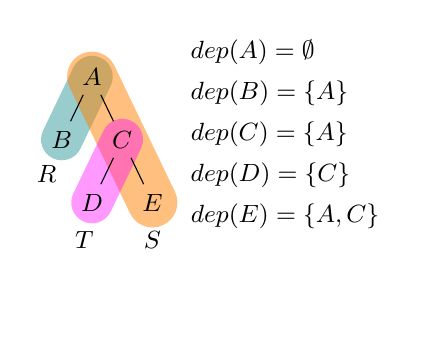
\begin{tikzpicture}[xscale=0.96, yscale=0.8]
        \node at (0, 0.0) (A) {\small  $A$};
        \node at (-0.4, -1.0) (B) {\small $B$} edge[-] (A);
        \node at (0.4, -1.0) (C) {\small $C$} edge[-] (A);
        \node at (0.8, -2.0) (E) {\small $E$} edge[-] (C);
        \node at (0, -2.0) (D) {\small $D$} edge[-] (C);
        \node at (0.8, -2.6) (S) {\small $S$};
        \node at (-0.6, -1.55) (R) {\small  $R$};
        \node at (-0.1, -2.6) (T) {\small  $T$};
        \node at (2.55, -1.6) {
          \small
          \begin{tabular}{@{~~}l}
            $dep(A) = \emptyset$\\[1ex]
            $dep(B)=\{A\}$\\[1ex]
            $dep(C)=\{A\}$\\[1ex]
            $dep(D)=\{C\}$\\[1ex]
            $dep(E)=\{A,C\}$\\[8ex]
          \end{tabular}
        };
      
        \begin{pgfonlayer}{background}
          \draw[opacity=.4,fill opacity=.4,line cap=round, line join=round, line width=15pt,color=teal] (0,0.0) -- (-0.4,-1);
          \draw[opacity=.5,fill opacity=.5,line cap=round, line join=round, line width=18pt,color=orange] (0,0.0) -- (0.8,-2.0);
          \draw[opacity=.4,fill opacity=.4,line cap=round, line join=round, line width=15pt,color=purple]  (0.4,-1) -- (0, -2.0);
        \end{pgfonlayer}
      \end{tikzpicture}
      }
  \end{minipage}
  % 
  \begin{minipage}[b]{0.32\linewidth}
    % \scalebox{0.95}{
    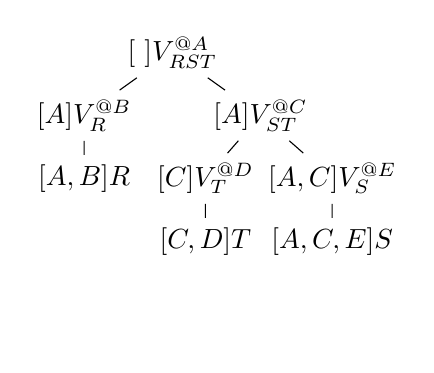
\begin{tikzpicture}[xscale=0.7, yscale=0.8]
      \node at (0, 0) (A) {$\VIEW[~]{V^{@A}_{RST}}$};
      \node at (-1.6, -1) (B) {$\VIEW[A]{V^{@B}_{R}}$} edge[-] (A);
      \node at (1.6, -1) (C) {$\VIEW[A]{V^{@C}_{ST}}$} edge[-] (A);
      \node at (0.6, -2) (D) {$\VIEW[C]{V^{@D}_{T}}$} edge[-] (C);
      \node at (2.9, -2) (E) {$\VIEW[A,C]{V^{@E}_{S}}$} edge[-] (C);
      
      \node at (-1.6, -2) {$\VIEW[A,B]{R}$} edge[-] (B);
      \node at (2.9, -3) {$\VIEW[A,C,E]{S}$} edge[-] (E);
      \node at (0.6, -3) {$\VIEW[C,D]{T}$} edge[-] (D);

      \node at (0.5, -4.5) {}; 
    \end{tikzpicture}
    % }
  \end{minipage}
  \begin{minipage}[b]{0.3\linewidth}
    \begin{align*}
      &\VIEW[A,C]{V^{@E}_{S}} = \VSUM_{E} \VIEW[A,C,E]{S} \\[2pt]
      &\VIEW[C]{V^{@D}_{T}} = \VSUM_{D} \VIEW[C,D]{T} \\[2pt]
      &\VIEW[~]{V^{@A}_{RST}} = \VSUM_{A} \big(\VIEW[A]{V^{@B}_{R}} \VPROD \VIEW[A]{V^{@C}_{ST}}\big) \\[2pt]
      &\VIEW[A]{V^{@B}_{R}} = \VSUM_{B} \VIEW[A,B]{R} \\[2pt]
      &\VIEW[A]{V^{@C}_{ST}} = \VSUM_{C} \big(\VIEW[C]{V^{@D}_{T}} \VPROD \VIEW[A,C]{V^{@E}_{S}}\big)
      \\[0.5cm]
   \end{align*}  
  \end{minipage}  
  \vspace*{-0.7cm}
\caption{
(left) Variable order $\omega$ of the natural join of the relations $\VIEW[A,B]{R}$, $\VIEW[A,C,E]{S}$, and $\VIEW[C,D]{T}$; (middle) View tree over $\omega$ and $\mathcal{F} = \emptyset$;
(right)  View definitions. 
}
\label{fig:example_payloads}
% \vspace*{-1em}
\end{figure}


%%%%%%%%%%%%%%%%%%%%%%%%%%%%%%%%%%%%

\paragraph{\textbf{Variable Orders.}}
Classical query evaluation makes use of  query plans that dictate the order in which the relations are joined. We use a different evaluation approach based on variable orders that dictate the  order in which we marginalize each join variable. This approach may require to join several relations at a time if they have the same variable. Our choice is motivated by the complexity of the evaluation problem for join queries: standard (relation-at-a-time) query plans are provably suboptimal, whereas the evaluation by variable orders can be worst-case optimal~\cite{Ngo:SIGREC:2013}.

Given a join query $Q$, a variable $X$ {\em depends} on a variable $Y$ if both are in the schema of a relation in $Q$.

\begin{definition}[adapted from \cite{Olteanu:FactBounds:2015:TODS}]\label{def:vo}
A {\em variable order} $\omega$ for a join query $Q$ is a pair $(F,dep)$, where $F$ is a rooted forest with one node per variable in $Q$, and {\em dep} is a function mapping each variable $X$ to a set of variables in $F$. It satisfies the following constraints:
\begin{itemize}
\item For each relation in $Q$, all of its variables lie along a root-to-leaf path in $F$.
%  
\item For each variable $X$, $dep(X)$ is the subset of its ancestors in $F$ on which the variables in the subtree rooted at $X$ depend.
\end{itemize}
\end{definition}

\begin{example}
Consider the query
%$\VIEW[~]{Q} = \VSUM_A\VSUM_B\VSUM_C\VSUM_D\VSUM_E \VIEW[A,B]{R}  \VPROD \VIEW[A,C,E]{S} \VPROD \VIEW[C,D]{T}$
from Example~\ref{ex:sql_count} that joins the relations $\VIEW{R}[A,B]$, $\VIEW[A,C,E]{S}$, and 
$\VIEW[C,D]{T}$.   
Figure~\ref{fig:example_payloads}  gives a variable order (top left) for
the query.
  Variable $D$ has ancestors $A$ and $C$, yet it only depends on $C$ since $C$ and $D$ appear in the same relation $\VIEW[]{T}$ and $D$ does not occur in any relation together with $A$. Thus, $dep(D)=\{C\}$. Given $C$, the variables $D$ and $E$ are independent of each other.
\punto
\end{example}
For a query $Q$ with free variables, a variable order is \emph{free-top} if no bound variable is an ancestor of a free variable~\cite{KNOZ20}. Variable orders are a different syntax~\cite{Olteanu:FactBounds:2015:TODS} for hypertree decompositions~\cite{Gottlob99}. They are more natural for algorithms that proceed one variable at a time.

%\paragraph{\textbf{View Trees.}}
\textbf{View Trees.} Our framework relies on a variable order $\omega$ for the input query $Q$ to describe the structure of the computation and indicate which variable marginalizations are pushed past joins. Based on $\omega$, we construct a tree of views that represent \DF's data structure to support query maintenance and enumeration.

\begin{figure}[t]
\centering
\setlength{\tabcolsep}{3pt}
\renewcommand{\arraystretch}{1.2}
\begin{tabular}{@{}c@{}c@{~~~}l}
  \toprule
  \multicolumn{3}{c}{$\tau$(\text{variable order} $\omega$, \text{free variables} $\mathcal{F}$) : view tree} \\
  \midrule
  \multicolumn{3}{l}{\MATCH $\omega$:} \\
  \midrule 
  \phantom{a} & $\VIEW{R}$\hspace*{1em} & \RETURN $\VIEW[\mathit{\sch(\VIEW{R})}]{R}$ \\
  \cmidrule{2-3} \\[-6pt] 
  &
  \begin{minipage}[b]{1.8cm}
    \begin{tikzpicture}[xscale=0.4, yscale=1]
      \node at (0,-2)  (n4) {$X$};
      \node at (-1,-3)  (n1) {$\omega_1$} edge[-] (n4);
      \node at (0,-3)  (n2) {$\ldots$};
      \node at (1,-3)  (n3) {$\omega_k$} edge[-] (n4);
      \node at (0,-4.5) {~};
    \end{tikzpicture}
    \vspace{1.5cm}
  \end{minipage}
  &
  \begin{minipage}[b]{6.3cm}
\LET $T_i = \tau(\omega_i, \mathcal{F}), \ \forall i\in[k] $\\[0.5ex]  
  \LET $\VIEW[\mathit{keys_i}]{V^{@\omega_i}_{rels_i}} = \text{ root of } T_i, \ \forall i\in[k] $\\[0.5ex]
    \LET $\mathit{keys}=\mathit{dep}(X) \cup (\mathcal{F} \cap \vars(\omega))$ \\[0.5ex]
    \LET $\mathsf{rels}=\bigcup_{i\in[k]}\mathsf{rels}_i$\\[0.5ex]
    \IF $X \notin \mathcal{F}$ \\[0.5ex]
    \TAB $\VIEW[\mathit{keys}]{V^{@X}_{rels}}= \VSUM_{X} \VPRODBIG_{i \in [k]} \VIEW[\mathit{keys_i}]{V^{@\omega_i}_{rels_i}}$\\[0.5ex]
    \ELSE \\[0.5ex]
    \TAB $\VIEW[\mathit{keys}]{V^{@X}_{rels}}=\VPRODBIG_{i \in [k]} \VIEW[\mathit{keys_i}]{V^{@\omega_i}_{rels_i}}$\\[0.5ex]
    \RETURN $
				\left\{
				\begin{array}{@{~~}c@{~~}}
					\tikz {
						\node at (1.2,-1)  (n4) {$\VIEW[\mathit{keys}]{V^{@X}_{rels}}$};
						\node at (0.8,-1.75)  (n1) {$T_1$} edge[-] (n4);
						\node at (1.25,-1.75)  (n2) {$\ldots$};
						\node at (1.8,-1.75)  (n3) {$T_k$} edge[-] (n4);
					}
				\end{array}  \right.$
  \end{minipage}
  \\
  \bottomrule
\end{tabular}
% \vspace*{-1em}
\caption{Creating a view tree $\tau(\omega, \mathcal{F})$ for a variable order $\omega$ and a set of free variables $\mathcal{F}$.}
\label{fig:static_view_tree_algo}
% \vspace*{-1.45em}
\end{figure}

Figure~\ref{fig:static_view_tree_algo} gives a function $\tau$ that constructs a view tree $\tau$ for a variable order $\omega$ and the set $\mathcal{F}$ of free variables of the query $Q$. Without loss of generality, we assume that $\omega$ is a single rooted tree. Otherwise, we apply $\tau$  to each tree in $\omega$ to obtain a set of view trees.
For simplicity, we assume that $\omega$ was first extended with relations as children under their lowest variable. 

The function  $\tau$ maps the variable order to a view tree of the same tree structure, yet with each variable $X$ replaced by a view $\VIEW[keys]{V^{@X}_{rels}}$. This notation states that the view $\VIEW{V}$ is (recursively) defined over the input relations {\sf rels}, has free variables $keys$, and it corresponds to the variable $X$ in $\omega$; in case of a view for an input relation $\VIEW{R}$, we use the simplified notation $\VIEW[\sch(\VIEW{R})]{R}$.

The base case (leaf in the extended variable order) is that of an input relation: We construct a view that is the relation itself. At a variable $X$ (inner node), we distinguish two cases: If $X$ is a bound variable, then we construct a view that marginalizes out $X$ in the natural join of the views that are children of the current view; we thus first join on $X$, then apply the lifting function for $X$ on its values, and aggregate $X$ away. If $X$ is a free variable, however, then we retain it in the view schema without applying the lifting function to its values. The schema of the view consists of $dep(X)$ and the free variables in the subtree of $\omega$ rooted at $X$.

\begin{figure}[t]
  \centering
  \begin{tikzpicture}
        \node at (0, 0.5) (x) {
    \begin{minipage}[b]{0.2\linewidth}
      \small
  %  \scalebox{0.95}{   
      \hspace{-0.25cm}
      \begin{tikzpicture}[xscale=0.8, yscale=0.24]  
        \node at (0, -1.5) (A) {$\VIEW[A,C]{V^{@A}_{RST}}$};
        \node at (-1.5, -5) (B) {$\VIEW[A]{V^{@B}_{R}}$} edge[-] (A);
        \node at (1.5, -5) (C) {$\VIEW[A,C]{V^{@C}_{ST}}$} edge[-] (A);
        \node at (0.5, -9) (D) {$\VIEW[C]{V^{@D}_{T}}$} edge[-] (C);
        \node at (2.5, -9) (E) {$\VIEW[A,C]{V^{@E}_{S}}$} edge[-] (C);
        
        \node at (-1.5, -8) {$\VIEW[A,B]{R}$} edge[-] (B);
        \node at (2.5, -12) {$\VIEW[A,C,E]{S}$} edge[-] (E);
        \node at (0.5, -12) {$\VIEW[C,D]{T}$} edge[-] (D);
  \end{tikzpicture}
  % }
    \end{minipage}
    };

        \node at (8.2, 0.5) (x) {
     \begin{minipage}[b]{0.3\linewidth}       
      % \scalebox{0.95}{\parbox{\linewidth}{%
        \begin{align*}
          &\VIEW[A,C]{V^{@A}_{RST}} = \VIEW[A]{V^{@B}_{R}} \VPROD \VIEW[A,C]{V^{@C}_{ST}} \\[2pt]
          &\VIEW[A,C]{V^{@C}_{ST}} = \VIEW[C]{V^{@D}_{T}} \VPROD \VIEW[A,C]{V^{@E}_{S}} \\[2pt]
          &\VIEW[A,C]{V^{@E}_{S}} = \VSUM_{E} \VIEW[A,C,E]{S} \\[2pt]
          &\VIEW[A]{V^{@B}_{R}} =  \VSUM_{B}\VIEW[A,B]{R} \\[2pt]
          &\VIEW[C]{V^{@D}_{T}} =  \VSUM_{D}\VIEW[C,D]{T}
        \end{align*}
      % }}    
    \end{minipage}
};
\end{tikzpicture}    
  \caption{
  (left) View tree over the variable order $\omega$ in Figure~\ref{fig:example_payloads} and 
  $\mathcal{F} = \{A,C\}$; (right) View definitions.
  }
  \label{fig:view tree_free_vars}
  % \vspace*{-1em}
\end{figure}

\begin{figure}[t]
  \begin{minipage}[b]{\linewidth}
    \centering
    \small
    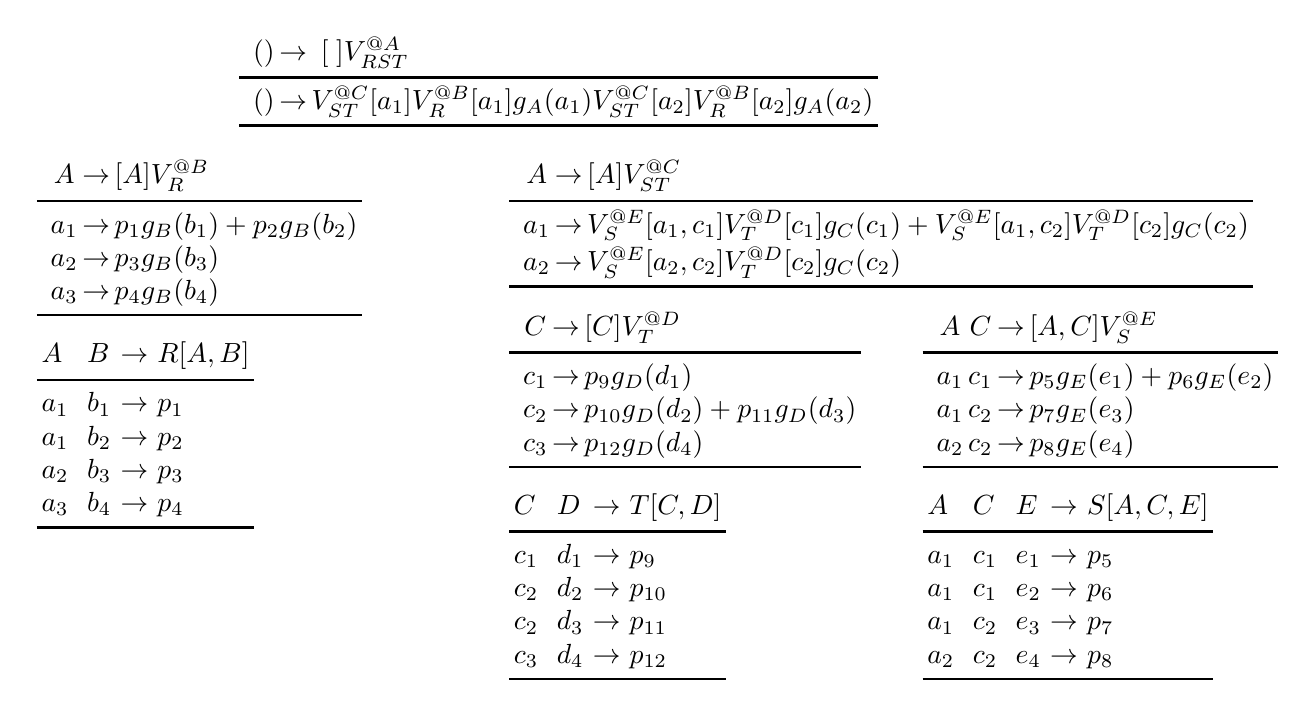
\begin{tikzpicture}[xscale=0.75, yscale=0.35]         
    
      % at node A
      \node at (2, 0) {
        \begin{tabular}{@{\,}l@{\,}  @{\,}c@{\,}c@{\,}l@{\,}}
          & $()$ & $\rightarrow$ & \ $\VIEW[\;]{V^{@A}_{RST}}$ \\[0.5ex]\toprule
          & $()$ & $\rightarrow$ & 
          $\VIEW{V^{@C}_{ST}}[a_1] \RINGPROD \VIEW{V^{@B}_{R}}[a_1] \RINGPROD g_A(a_1) \RINGPLUS \VIEW{V^{@C}_{ST}}[a_2] \RINGPROD \VIEW{V^{@B}_{R}}[a_2] \RINGPROD g_A(a_2) $           
          \\\bottomrule
        \end{tabular}
      };   

      % at node B
      \node[anchor=north west] at (-7, -2.5) {
        \begin{tabular}{@{\,}l@{\,} @{\,}c@{\,}c@{\,}l@{\,}}
          %  
          & $A$ & $\to$ & $\VIEW[A]{V^{@B}_{R}}$ \\[0.5ex]\toprule
          & $a_1$ & $\rightarrow$ & $p_{1} \RINGPROD  g_B(b_1)  + p_{2} \RINGPROD  g_B(b_2)$ \\
          & $a_2$ & $\rightarrow$ & $p_{3} \RINGPROD  g_B(b_3)$ \\
          & $a_3$ & $\rightarrow$ & $p_{4} \RINGPROD  g_B(b_4)$\\\bottomrule
        \end{tabular}
      };
      
      % at node R
      \node[anchor=north west] at (-7, -9) {
      \begin{tabular}{@{\,}l@{~~}l@{~$\to$~}l@{\,}}
        $A$ & $B$ & $\VIEW{R}[A,B]$\\[0.5ex]\toprule
        $a_1$ & $b_1$ & $p_1$ \\
        $a_1$ & $b_2$ & $p_2$\\  
        $a_2$ & $b_3$ & $p_3$\\
        $a_3$ & $b_4$ & $p_4$\\\bottomrule
        \end{tabular}
      };

      % at node C
      \node [anchor=north west] at (1, -2.5) {
        \begin{tabular}{@{\,}l@{\,} @{\,}c@{\,}c@{\,}l@{\,}}
          & $A$ & $\rightarrow$ & $\VIEW[A]{V^{@C}_{ST}}$ \\[0.5ex]\toprule
          & $a_1$ & $\rightarrow$ & 
          $\VIEW{V^{@E}_{S}}[a_1,c_1] \RINGPROD \VIEW{V^{@D}_{T}}[c_1] \RINGPROD g_C(c_1) + 
          \VIEW{V^{@E}_{S}}[a_1,c_2] \RINGPROD \VIEW{V^{@D}_{T}}[c_2] \RINGPROD g_C(c_2)$ \\[0.05cm]  
          & $a_2$ & $\rightarrow$ & $\VIEW{V^{@E}_{S}}[a_2,c_2] \RINGPROD \VIEW{V^{@D}_{T}}[c_2] \RINGPROD g_C(c_2)$ \\
          \bottomrule 
        \end{tabular}
      };

      % at node D
      \node [anchor=north west] at (1, -8) {
        \begin{tabular}{@{\,}l@{\,} @{\,}c@{\,}c@{\,}l@{\,}}
          %  
          & $C$ & $\to$ & $\VIEW[C]{V^{@D}_{T}}$ \\[0.5ex]\toprule
          & $c_1$ & $\rightarrow$ & $ p_9 \RINGPROD g_D(d_1)$\\
          & $c_2$ & $\rightarrow$ & $p_{10} \RINGPROD  g_D(d_2)  + p_{11} \RINGPROD  g_D(d_3)$ \\
          & $c_3$ & $\rightarrow$ & $p_{12} \RINGPROD  g_D(d_4)$ \\\bottomrule
        \end{tabular}
      };

      % at node E
      \node [anchor=north west] at (8, -8) {
        \begin{tabular}{@{\,}l@{\,} @{\,}c@{\,}c@{\,}c@{\,}l@{\,}}
          & $A$ & $C$ & $\to$ & $\VIEW[A,C]{V^{@E}_{S}}$ \\[0.5ex]\toprule
          & $a_1$ & $c_1$ & $\rightarrow$ & $p_{5} \RINGPROD  g_E(e_1)  + p_{6} \RINGPROD  g_E(e_2)$ \\
          & $a_1$ & $c_2$ & $\rightarrow$ & $p_{7} \RINGPROD  g_E(e_3)$  \\
          & $a_2$ & $c_2$ & $\rightarrow$ & $p_{8} \RINGPROD  g_E(e_4) $ \\\bottomrule
        \end{tabular}
      };
      
      % at node T
      \node [anchor=north west] at (1, -14.5) {
       \begin{tabular}{@{\,}l@{~~}l@{~$\to$~}l@{\,}}
        $C$ & $D$ & $\VIEW{T}[C,D]$ \\[0.5ex]\toprule
        $c_1$ & $d_1$ & $p_9$\\
        $c_2$ & $d_2$ & $p_{10}$\\
        $c_2$ & $d_3$ & $p_{11}$\\
        $c_3$ & $d_4$ & $p_{12}$\\\bottomrule
      \end{tabular}
      };

      % at node S
      \node [anchor=north west] at (8, -14.5) {
      \begin{tabular}{@{\,}l@{~~}l@{~~}l@{~$\to$~}l@{\,}}
        $A$ & $C$ & $E$ & $\VIEW{S}[A,C,E]$ \\[0.5ex]\toprule
        $a_1$ & $c_1$ & $e_1$ & $p_5$\\
        $a_1$ & $c_1$ & $e_2$ & $p_6$\\
        $a_1$ & $c_2$ & $e_3$ & $p_7$\\
        $a_2$ & $c_2$ & $e_4$ & $p_8$\\\bottomrule
      \end{tabular}
      };
    \end{tikzpicture}
  \end{minipage}
\caption{
Contents of the views in the view tree from Figure~\ref{fig:example_payloads} in case the relations 
$\VIEW{R}$,
$\VIEW{S}$, and $\VIEW{T}$ are over a ring 
$(\RING, \RINGPLUS, \RINGPROD, \RINGZERO, \RINGONE)$ with $p_i \in \RING$ for
$i \in [12]$.}
\label{fig:count}
\end{figure}

\begin{example}
\label{ex:views_count}
Figure~\ref{fig:example_payloads} shows the view tree constructed by the function $\tau$ from 
Figure~\ref{fig:static_view_tree_algo} over the variable order $\omega$ and the empty set of free variables.
Figure~\ref{fig:view tree_free_vars} depicts 
  the view tree constructed over the
  same variable order but for 
the set  $\mathcal{F} = \{A,C\}$ of free variables.
  
Figure~\ref{fig:count} gives the  
  contents of the views in the view tree from Figure~\ref{fig:example_payloads}, where 
$\VIEW{R}$,
$\VIEW{S}$, and $\VIEW{T}$ are relations over a ring $\RING$ with payloads $p_i \in \RING$ for
$i \in [12]$. 
Assume that $\RING$ is the $\mathbb{Z}$ ring, 
each tuple in these relations 
is mapped to $1$,
i.e.,  $p_i = 1$ for $i \in [12]$, and 
the lifting functions map all
values to $1$.
Then, the view tree 
computes the {\tt COUNT} query 
from Example~\ref{ex:sql_count}
and the root view $\VIEW{V_{RST}^{@A}}$ maps the empty tuple to 
  the overall count $10$,
which is the number 
of tuples in the natural join of $\VIEW{R}$, $\VIEW{S}$, and 
$\VIEW{T}$.
\punto
\end{example}

By default, the function $\tau$ in Figure~\ref{fig:static_view_tree_algo} constructs one view per variable in the variable order $\omega$. A wide relation (with many variables) leads to long branches in $\omega$ with variables that are only local to this relation. This is, for instance, the case of our retailer dataset used in 
Section~\ref{sec:experiments}. Such long branches create long chains of views, where each view marginalizes one bound variable over its child view in the chain. For practical reasons, we compose such long chains into a single view that marginalizes several variables at a time. 

  
\input{factorized_ivm}
%%%%%%%%%%%%%%%%%%%%%%%%%%%%%%%
\section{Factorizable Updates}
\label{sec:factorizable_updates}

Our focus so far has been on supporting updates represented by delta relations. We next consider an alternative approach that decomposes a delta relation into a union of factorizable relations. The cumulative size of the decomposed relations can be much less than the size of the original delta relation. Also, the complexity of propagating a factorized update can be much lower than that of its unfactorized (listing) representation, since the factorization makes explicit the independence between query variables and enables optimizations of delta propagation such as pushing marginalization past joins. Besides the factorized view computation, this is the second instance where \DF exploits factorization.

Factorizable updates arise in many domains such as linear algebra and machine learning. Section~\ref{sec:applications} demonstrates how our framework can be used for the incremental evaluation of matrix chain multiplication, recovering prior work on this~\cite{NEK:SIGMOD:2014}.  Matrix chain computation can be phrased in our language of joins and aggregates, where matrices are binary relations. Changes to one row/column in an input matrix may be expressed as a product of two vectors. In general, an arbitrary update matrix can be decomposed into a sum of rank-$1$ matrices, each of them  expressible as products of vectors, using low-rank tensor decomposition methods~\cite{TensorDecomp:2009,TensorDecomposition:2017}.

\begin{example}
Arbitrary relations can be decomposed in\-to a union of factorizable relations. The relation $\VIEW[A,B]{R}$ $= \{(a_i,b_j) \to 1\mid i\in[n],j\in[m]\}$ can be decomposed as $\VIEW[A]{R_1}\VPROD\VIEW[B]{R_2}$, where $\VIEW[A]{R_1}=\{(a_i) \to 1\mid i\in[n]\}$ and $\VIEW[B]{R_2}=\{(b_j) \to 1\mid j\in[m]\}$. We thus reduced a relation of size $nm$ to two relations of cumulative size $n+m$. If $\VIEW{R}$ were a delta relation, the delta views on top of it would now be expressed over $\VIEW[A]{R_1}\VPROD\VIEW[B]{R_2}$ and their computation can be factorized as done for queries in Section~\ref{sec:factorized_ring_computation}. Product decomposition of relations can be done in linearithmic time in both the number of variables and the size of the relation~\cite{WSD:2008}. 

Consider now $\VIEW[A,B]{R'}$ $=$ $\VIEW[A,B]{R}$ $\VPLUS$ $\{(a_{n+1},b_j) \to 1\mid j\in[m-1]\}$ with $\VIEW{R}$ as above. We can decompose each of the two terms in $\VIEW{R'}$ similarly to $\VIEW{R}$, yielding overall $n+2m$ values instead of $nm+m-1$. A different decomposition with $n+m+3$ values is given by a factorizable over-approximation of $\VIEW{R'}$ compensated by a small product with negative payload: $\{(a_i)\to 1\mid i\in[n+1]\}\VPROD\{(b_j)\to 1\mid j\in[m]\}\VPLUS\{(a_{n+1})\to 1\}\VPROD\{(b_m)\to -1\}$.\punto
\end{example}

The {\sc Optimize} method used in the delta view tree algorithm in Figure~\ref{fig:dynamic_view_tree_algo} exploits the distributivity of join $\VPROD$ over marginalization $\VSUM_{X}$ to push the latter past the former and down to the views with variable $X$. This optimization is reminiscent of pushing aggregates past joins in databases and variable elimination in probabilistic graphical models~\cite{FAQ:PODS:2016}. In case the delta views express Cartesian products, then they are not materialized but instead kept factorized.

\begin{example}
\label{ex:factorized-update}
Consider the query $\VIEW{Q}$ from Example~\ref{ex:delta_view_tree} 
and its view tree in Figure~\ref{fig:example_payloads}.
In the delta view tree derived for updates to $\VIEW{S}$, the top-level delta is computed as:
\begin{align*}
\VIEW[~]{\delta{V^{@A}_{RST}}} = \VSUM_{A} \VIEW[A]{V^{@B}_{R}} \VPROD 
\big(&  \VSUM_{C} \VIEW[C]{V^{@D}_{T}} \VPROD \\
& \underbrace{\hspace{3em}\underbrace{\VSUM_{E} \VIEW[A,C,E]{\delta{S}}}_{\VIEW[A,C]{\delta{V^{@E}_{S}}}}\big)}_{\VIEW[A]{\delta{V^{@C}_{ST}}}}
\end{align*}
A single-tuple update $\VIEW{\delta{S}}$ binds variables $A$, $C$, and $E$, and computing $\VIEW{\delta{V^{@A}_{RST}}}$ requires $\bigO{1}$ lookups in $\VIEW{V^{@D}_{T}}$ and $\VIEW{V^{@B}_{R}}$. An arbitrary-sized update $\VIEW{\delta{S}}$ can then be processed in $\bigO{|\VIEW{\delta{S}}|}$ time.

Assume now that $\VIEW{\delta{S}}$ is factorizable as $\VIEW[A,C,E]{\delta{S}} = \VIEW[A]{\delta{S_{A}}} \VPROD \VIEW[C]{\delta{S_{C}}} \VPROD \VIEW[E]{\delta{S_{E}}}$. In the construction of the delta view tree, the {\sc Optimize} method exploits this factorization to push the marginalization past joins at each variable; for example, the delta at $E$ becomes:
\begin{align*}
\VIEW[A,C]{\delta{V^{@E}_{S}}} &= \VSUM_{E} \VIEW[A]{\delta{S_{A}}} \VPROD \VIEW[C]{\delta{S_{C}}} \VPROD \VIEW[E]{\delta{S_{E}}} \\
&= \VIEW[A]{\delta{S_{A}}} \VPROD \VIEW[C]{\delta{S_{C}}} \VPROD \VSUM_{E} \VIEW[E]{\delta{S_{E}}}
\end{align*}
We also transform the top-level delta into a product of three views:
\begin{align*}
\VIEW[~]{\delta{V^{@A}_{RST}}} = 
&\big( \VSUM_{A} \VIEW[A]{V^{@B}_{R}} \VPROD \VIEW[A]{\delta{S_{A}}} \big) \VPROD
\big( \VSUM_{C} \VIEW[C]{V^{@D}_{T}} \VPROD \VIEW[C]{\delta{S_{C}}} \big) \VPROD 
 \big( \VSUM_{E} \VIEW[E]{\delta{S_{E}}} \big)
\end{align*}
The computation time for this delta is proportional to the sizes of the three views representing the update:
$\bigO{\min(|\VIEW{V^{@B}_{R}}|, {|\VIEW{\delta{S_{A}}}|}) + \min(|\VIEW{V^{@D}_{T}}|, |\VIEW{\delta{S_{C}}}|) + |\VIEW{\delta{S_{E}}}|}$.
\punto
\end{example}



\section{\DF for Special Query Classes}

\label{sec:query_classes}

This section shows how \DF maintains {\em free-connex ($\alpha$-)acyclic} queries~\cite{DynYannakakis:SIGMOD:2017} and {\em $q$-hierarchical} queries~\cite{Nicole:PODS:2017}. The analysis for these queries is refined into: (i) the preprocessing phase, where the view tree is constructed; (ii) the enumeration phase, where we present the query result one tuple at a time; and (iii) the update phase, where we update the view tree. The following data complexity\footnote{The {\em data complexity} is a function of the database size.} claims assume that the ring operations require constant time, otherwise the complexity results stated in this section have an extra multiplying factor to account for the complexity of the ring operations.


\begin{theorem}\label{th:special-cases}
  Let a query $\VIEW[]{Q}$ and a database of size $N$.

  \DF can maintain $\VIEW[]{Q}$ with $O(N)$ preprocessing, $O(1)$ enumeration delay, and $O(N)$ single-tuple update in case $\VIEW[]{Q}$ is free-connex acyclic.
  
  \DF can maintain $\VIEW[]{Q}$ with $O(N)$ preprocessing, $O(1)$ enumeration delay, and $O(1)$ single-tuple update in case $\VIEW[]{Q}$ is $q$-hierarchical.
\end{theorem}

Section~\ref{sec:cyclic_queries} discusses an important extension of our view tree construction to better support cyclic queries.

% % \begin{remark}
% {\it Remark.}
% \DF has a special treatment for cyclic que\-ries.
% % which is not discussed in this article for lack of space.
% Whereas for acyclic join queries the size of each view is asymptotically upper-bounded by the size of the query result, for cyclic queries views may be larger than the query result. 
% In prior work~\cite{FIVM:SIGMOD:2018}, we show how to reduce the size of intermediate views for cyclic queries  by adding indicator projections~\cite{FAQ:PODS:2016} to 
% view trees.  Such projections do not effect the query result but can constrain views (e.g., create cycles) and bring asymptotic savings in space and time.
% To decide which indicator projections to use, we apply a variant of the \textsf{GYO} reduction~\cite{BeeriFMY83} that discovers cyclic parts in the query.  
% \punto  
% % \end{remark}


\subsection{Free-Connex Acyclic Queries}
\label{sec:free-connex}

We first introduce the class of free-connex acyclic que\-ries and then explain how \DF maintains them.

\begin{definition}[\cite{Yannakakis81,BraultPhD13}]
  A {\em join tree} for a query is a tree, where each node is a relation and if any two nodes have variables in common, then all nodes along the path between them also have these variables. 

  A query is \emph{($\alpha$-)acyclic} if it admits a join tree.
  % where each node is a relation and if any two nodes have variables in common, then all nodes along the path between them also have these variables. 
  %
  A query is \emph{free-connex acyclic} if it is acyclic and remains acyclic after adding a new relation whose schema consists of the free variables of the query. 
\end{definition}

\begin{example}
\label{ex:acyclic}
Consider the query 
$\VIEW[A,B,C]{Q} = \VSUM_{D}\VSUM_{E}$ $\VIEW[A,B]{R} \VPROD \VIEW[A,C,E]{S} \VPROD \VIEW[C,D]{T}$. 
  A possible join tree for $\VIEW[]{Q}$ is 
  $\VIEW[A,B]{R} - \VIEW[A,C,E]{S} - \VIEW[C,D]{T}$, where 
  ``$-$" denotes the parent-child relationship.
  Hence, $\VIEW[]{Q}$ is acyclic. 
  
Consider the triangle query 
$\VIEW[~]{Q_{\vartriangle}} = \VSUM_{A}\VSUM_{B}\VSUM_{C}$ $\VIEW[A,B]{R} \VPROD \VIEW[B,C]{S} \VPROD \VIEW[A,C]{T}$. A possible tree built from the relations  
of $\VIEW[]{Q_{\vartriangle}}$ is
$\VIEW[A,B]{R} - \VIEW[B,C]{S} - \VIEW[A,C]{T}$.    
The variable $A$ occurs in the first and last relations but not in the middle relation; thus, this tree is not a join 
tree for $\VIEW[]{Q_{\vartriangle}}$. One can show that any 
tree built from the relations of $\VIEW[]{Q_{\vartriangle}}$ is not a join tree. 
Hence, $\VIEW[]{Q_{\vartriangle}}$ is not acyclic.


The tree $\VIEW[A,B]{R} - \VIEW[A,B,C]{U} - \VIEW[A,C,E]{S} - \VIEW[C,D]{T}$
is a join tree of $\VIEW[]{Q}$ extended with the relation 
$U$ whose schema consists of the free variables of $\VIEW[]{Q}$.
Hence, $\VIEW[]{Q}$ is free-connex acyclic. 
Consider now the variant $\VIEW[]{Q'}$ 
of $\VIEW[]{Q}$ where only the variables $B$ and $C$ are free.
Adding a fresh relation $U'$ with schema $(B,C)$ to 
$\VIEW[]{Q'}$ turns it into a cyclic query $\VIEW[]{Q''}$
that does not admit a join tree. 
\punto
\end{example}

\begin{figure}[t]
\centering
\setlength{\tabcolsep}{3pt}
%
\begin{tabular}{@{}c@{}c@{~~~}l}
  \toprule
  \multicolumn{3}{c}{$\nu$ (\text{free-top variable order} $\omega$) : view tree} \\
  \midrule
  \multicolumn{3}{l}{\MATCH $\omega$:} \\
  \midrule 
  \phantom{a} & $\VIEW{R}$\hspace*{2.5em} & \RETURN $\VIEW[\mathit{\sch(\VIEW{R})}]{R}$ \\
  \cmidrule{2-3} \\[-6pt] 
  &
  \begin{minipage}[b]{2.5cm}
    \begin{tikzpicture}[xscale=0.4, yscale=1]
      \node at (0,-2)  (n4) {$X$};
      \node at (-1,-3)  (n1) {$\omega_1$} edge[-] (n4);
      \node at (0,-3)  (n2) {$\ldots$};
      \node at (1,-3)  (n3) {$\omega_k$} edge[-] (n4);
      \node at (0,-4.5) {~};
    \end{tikzpicture}
    \vspace{3.4cm}
  \end{minipage}
  &
\begin{minipage}[b]{6.5cm}
\LET $T_i  = \tau(\omega_i), \ \forall i\in[k] $\\[0.5ex]
\LET $\VIEW[\mathit{keys_i}]{V^{@\omega_i}_{rels_i}} = \text{ root of } T_i, \ \forall i\in[k] $\\[0.5ex]
\LET $\mathit{keys}=\{X\} \cup \mathit{dep}(X)$ \\[0.5ex]
\LET $\mathsf{rels}=\bigcup_{i\in[k]}\mathsf{rels}_i$\\[0.5ex]
\LET $\VIEW[\mathit{keys}]{H^{@X}_{rels}}= \VPRODBIG_{i \in [k]} \VIEW[\mathit{keys_i}]
{V^{@\omega_i}_{rels_i}}$\\[0.5ex]
\LET $\VIEW[\mathit{keys}\setminus \{X\}]{V^{@X}_{rels}}= \VSUM_{X} \VIEW[\mathit{keys}]{H^{@X}_{rels}}$\\[0.5ex]
\IF $X$ has more than one child ($k\geq 2$) \\[0.5ex]
  \TAB \IF $X$ has no sibling \\[0.5ex]
    \TAB\TAB\TAB \RETURN $
				\left\{
				\begin{array}{@{~~}c@{~~}}
					\tikz {
						\node at (1.4,-1)  (n4) {$\VIEW[\mathit{keys}]{H^{@X}_{rels}}$};
						\node at (0.8,-1.75)  (n1) {$T_1$} edge[-] (n4);
						\node at (1.25,-1.75)  (n2) {$\ldots$};
						\node at (1.8,-1.75)  (n3) {$T_k$} edge[-] (n4);
					}
				\end{array}  \right.$  \\[0.5ex]
    \TAB\ELSE \\[0.5ex]
    \TAB\TAB\TAB\RETURN $
				\left\{
				\begin{array}{@{~~}c@{~~}}
					\tikz {
						\node at (1.2,-0.25)  (n) {$\VIEW[\mathit{keys}\setminus \{X\}]{V^{@X}_{rels}}$};
						\node at (1.2,-1)  (n4) {$\VIEW[\mathit{keys}]{H^{@X}_{rels}}$} edge[-] (n);
						\node at (0.8,-1.75)  (n1) {$T_1$} edge[-] (n4);
						\node at (1.25,-1.75)  (n2) {$\ldots$};
						\node at (1.8,-1.75)  (n3) {$T_k$} edge[-] (n4);
					}
				\end{array}  \right.$ \\[0.5ex]
\ELSE \\[0.5ex]        
  \TAB \IF $X$ has no sibling \\[0.5ex]
    \TAB\TAB\TAB \RETURN $T_1$ \\[0.5ex]
  \TAB\ELSE \\[0.5ex]
    \TAB\TAB\TAB\RETURN $
				\left\{
				\begin{array}{@{~~}c@{~~}}
					\tikz {
						\node at (1.2,-0.25)  (n) {$\VIEW[\mathit{keys}\setminus \{X\}]{V^{@X}_{rels}}$};
						\node at (1.2,-1)  (n1) {$T_1$} edge[-] (n);
					}
				\end{array}  \right.$      
  \end{minipage}
  \\
  \bottomrule
\end{tabular}
% \vspace*{-1em}
\caption{Creating a view tree for a free-top variable order.}
\label{fig:static_view_tree_algo_free-connex}
% \vspace*{-1.45em}
\end{figure}


We next detail how \DF achieves the complexity from Theorem~\ref{th:special-cases} for a free-connex acyclic query $\VIEW[]{Q}$. 

%\paragraph{\textbf{Preprocessing.}}
\textbf{Preprocessing.} 
In the preprocessing phase, we create a view tree
that compactly represent the result of $\VIEW[]{Q}$.
Given a variable order, the function $\tau$ in 
Figure~\ref{fig:static_view_tree_algo} constructs a view tree where
the root view consists of all tuples over the free variables.
While this view allows for constant enumeration delay, it may 
require superlinear computation and maintenance time as the free variables may originate from different input relations. We would like to avoid this super-linearity.

To keep the preprocessing and update times linear, we proceed as follows.
We construct view trees such that the query result is kept and maintained factorized over several views at the top of the view tree.
This approach still allows for constant enumeration delay, using a known enumeration approach for factorized representations~\cite{Olteanu:FactBounds:2015:TODS}.
We construct the view tree following a free-top variable order of the query $\VIEW[]{Q}$
and materialize a view over the schema $\{X\} \cup \mathit{dep}(X)$ for each variable $X$ in the variable order. 
A key insight is that every free-connex acyclic query admits a free-top variable order 
where for each variable $X$, the set $\{X\} \cup \mathit{dep}(X)$ 
is covered by the variables of a single relation~\cite{BerkholzGS20}. 
This ensures linear preprocessing and maintenance time for all views in view trees
following such variable orders.

The function  $\nu$ in Figure~\ref{fig:static_view_tree_algo_free-connex}
constructs a view tree for a given free-top variable 
order of a free-connex query.
If a variable $X$ has at least two children, it proceeds as follows.
It creates at $X$ 
a view $\VIEW[]{H^{@X}_{rels}}$ 
with schema $\{X\} \cup \mathit{dep}(X)$
that joins the child views of $X$.
If $X$ has at least one sibling, it additionally 
creates a view $\VIEW[]{V^{@X}_{rels}}$ on top of $\VIEW[]{H^{@X}_{rels}}$
obtained from $\VIEW[]{H^{@X}_{rels}}$ by marginalizing  $X$.
 The first view 
enables efficient enumeration of $X$-values in the query result given a value tuple 
 over $\mathit{dep}(X)$; the second view enables efficient updates 
coming from the subtrees rooted at siblings of $X$.  
If $X$ has only one child, the creation of the view $\VIEW[]{H^{@X}_{rels}}$ is not needed for efficient enumeration.
In this case, the function creates  a view $\VIEW[]{V^{@X}_{rels}}$ marginalizing $X$ in the child view if 
$X$ has siblings.  
 
\begin{example}\label{ex:free-connex-viewtree}
Consider the free-connex acyclic query 
$\VIEW[]{Q}$ from Example~\ref{ex:acyclic}.
Figure~\ref{fig:example_payloads} gives a free-top variable order $\omega$ for $\VIEW[]{Q}$. 
Figure~\ref{fig:free-connex_view_tree} (left) depicts 
the view tree $\nu(\omega)$. 
The view $\VIEW[]{H_{ST}^{@C}}$ can be computed by iterating 
over the $(A,C)$-tuples in $\VIEW[]{V_{S}^{@E}}$ and multiplying 
the payload of each such tuple with the payload of the matching 
$C$-value in $\VIEW[]{V_{T}^{@D}}$.   
Since each such $(A,C)$-tuple  must be in $\VIEW[]{S}$, we need to iterate 
over only linearly many such tuples.
Similarly, the view $\VIEW[]{H_{RST}^{@A}}$ can be computed by iterating 
over the $A$-values in one of the child views and doing lookups in the other child view to retrieve the payloads. For the computation of both views $\VIEW[]{H_{ST}^{@C}}$ and  $\VIEW[]{H_{RST}^{@A}}$,
we iterate over linearly  many 
tuples and do a constant-time lookup for each such tuple. 
All other views are obtained by marginalizing one variable from their child views. 
Hence, all views can be computed in linear time. 
\punto
\end{example}

\begin{figure}[t]
\centering
% \scalebox{0.87}{
  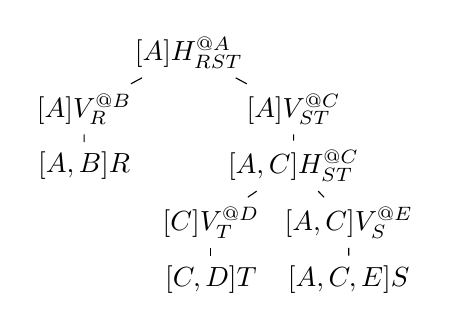
\begin{tikzpicture}[xscale=0.7, yscale=0.24]

    \node at (-0.4, 3) (A) {$\VIEW[A]{H^{@A}_{RST}}$};     
     \node at (1.5, 0) (C) {$\VIEW[A]{V^{@C}_{ST}}$} edge[-] (A);      
     \node at (1.5, -3) (C') {$\VIEW[A,C]{H^{@C}_{ST}}$} edge[-] (C);      
     \node at (2.5, -6) (E) {$\VIEW[A,C]{V^{@E}_{S}}$} edge[-] (C');
      \node at (2.5, -9) {$\VIEW[A,C,E]{S}$} edge[-] (E);
    
    \node at (0, -6) (D) {$\VIEW[C]{V^{@D}_{T}}$} edge[-] (C');
      \node at (0, -9) {$\VIEW[C,D]{T}$} edge[-] (D);  

      \node at (-2.3, -0) (B) {$\VIEW[A]{V^{@B}_{R}}$} edge[-] (A);
      \node at (-2.3, -3) {$\VIEW[A,B]{R}$} edge[-] (B);  
\end{tikzpicture}
% }
\hspace{0.5cm}
% \scalebox{0.87}{
  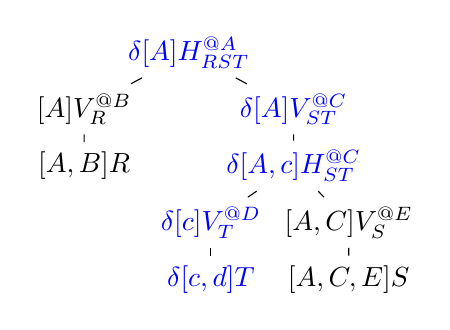
\begin{tikzpicture}[xscale=0.7, yscale=0.24]

    \node at (-0.4, 3) (A) {\color{blue} $\delta\VIEW[A]{H^{@A}_{RST}}$};     
     \node at (1.5, 0) (C) {\color{blue} $\delta\VIEW[A]{V^{@C}_{ST}}$} edge[-] (A);      
     \node at (1.5, -3) (C') {\color{blue} $\delta\VIEW[A,c]{H^{@C}_{ST}}$} edge[-] (C);      
     \node at (2.5, -6) (E) {$\VIEW[A, C]{V^{@E}_{S}}$} edge[-] (C');
      \node at (2.5, -9) {$\VIEW[A, C ,E]{S}$} edge[-] (E);
    
    \node at (0, -6) (D) {$\color{blue} \delta\VIEW[c]{V^{@D}_{T}}$} edge[-] (C');
      \node at (0, -9) {$\color{blue} \delta\VIEW[c,d]{T}$} edge[-] (D);  

      \node at (-2.3, -0) (B) {$\VIEW[A]{V^{@B}_{R}}$} edge[-] (A);
      \node at (-2.3, -3) {$\VIEW[A,B]{R}$} edge[-] (B);  
\end{tikzpicture}
% }
\caption{(left) View tree constructed by the function $\nu$ in 
Figure~\ref{fig:static_view_tree_algo_free-connex} for the variable 
order $\omega$ in Figure~\ref{fig:example_payloads};
(right) Delta view tree for a single-tuple update to $\VIEW{T}$.}
\label{fig:free-connex_view_tree}
% \vspace*{-1.45em}
\end{figure}

%\paragraph{\textbf{Updates}}
\textbf{Updates.} 
 The construction of delta view trees under single-tuple updates
 is exactly as described 
by the function $\Delta$ in Figure~\ref{fig:dynamic_view_tree_algo} (Section~\ref{sec:factorized_IVM}).
Since the view trees can be constructed in linear time, 
%and a single-tuple update to a relation fixes the variables of the relation schema
%in all ancestor views to constants, 
the delta view trees can also be constructed in linear time.

\begin{example}
Continuing Example~\ref{ex:free-connex-viewtree}, we consider a single-tuple update $\delta\VIEW{T}[c,d]$ to relation $\VIEW{T}$.
Figure~\ref{fig:free-connex_view_tree} depicts the original view tree (left) and the delta view tree for updates to $\VIEW{T}$ (right). The difference is that along the path from $\VIEW{T}$ to the root, we now have delta views.
The delta view $\delta\VIEW[]{V^{@D}_{T}}$
results from  $\delta\VIEW[c,d]{T}$ by marginalizing $D$, which takes  
constant time since $D$ is fixed to the constant $d$.
To compute $\delta\VIEW[]{H^{@C}_{ST}}$, we iterate over all $A$-values 
paired with $c$ in $\VIEW[]{V^{@E}_{S}}$. This operation takes linear time with the support of an index on variable $C$ built for this view.
% can be done in linear time with support of a tertiary index on variable $C$ for this view.
We obtain $\delta\VIEW[]{V^{@C}_{ST}}$ from $\delta\VIEW[]{H^{@C}_{ST}}$
by marginalizing the variable $C$. This requires constant time because $C$ is fixed to
the constant $c$. 
The top delta view $\delta\VIEW[]{H^{@A}_{RST}}$ is obtained by intersecting the two child views, e.g., by iterating over $\delta\VIEW[]{V^{@C}_{ST}}$ and doing lookups in $\VIEW[]{V^{@B}_R}$. This requires linear time. We conclude that the delta views can be computed in linear time. 
\punto
\end{example}

%\paragraph{\textbf{Enumeration.}}
\textbf{Enumeration.} 
Consider a view tree $\tau$ constructed using the function $\nu$ from 
Figure~\ref{fig:static_view_tree_algo_free-connex} for a free-top variable order of a 
query $\VIEW[]{Q}$. 
We first describe how to enumerate with constant delay the distinct tuples in the result of $\VIEW{Q}$ using $\tau$. Then, we explain how to compute the payload of each result tuple in constant time. 


Let $X_1, \ldots, X_n$ be an ordering of the free variables of the query
that is compatible with a top-down traversal of the free-top variable order. 
We use the views $\VIEW[]{V_1}, \ldots , \VIEW[]{V_n}$
%$\VIEW[]{H^{@X_1}}, \ldots , \VIEW[]{H^{@X_n}}$ 
to enumerate the distinct tuples
in the result of $\VIEW[]{Q}$, where 
$\VIEW[]{V_j}$ is $\VIEW[]{H^{@X_j}_{rels}}$ if $X_j$ has at least two children
and it is the child view of $X_j$ otherwise.  
We retrieve from $\VIEW[]{V_1}$ the first $X_1$-value in the 
result. 
When we arrive at a view  $\VIEW[]{V_j}$ with $j > 1$, we have already fixed 
the values of the variables above $X_j$ in the variable order. 
We retrieve from $\VIEW[]{V_j}$ the first $X_j$-value paired with these values. 
Once the values over all free variables 
are fixed, we have a complete result tuple that we output.
Then, we iterate over the remaining distinct $X_n$-values in $\VIEW[]{V_n}$
paired with the fixed values over the ancestor variables of $X_n$
and output a new tuple for each such value.
After all $X_n$-values are exhausted, we backtrack, i.e., we move to the next $X_{n-1}$-value
and restart the iteration of the matching $X_n$-values.      



\begin{figure}[t]
\centering
\setlength{\tabcolsep}{3pt}
%
\begin{tabular}{@{}c@{}c@{~~~}l}
  \toprule
  \multicolumn{3}{c}{$payload$(\text{view tree} $\tau$, \text{tuple} \textvec{t}): \text{payload}} \\
  \midrule
  \multicolumn{3}{l}{\MATCH $\tau$:} \\
  \midrule 
  \phantom{a} & $\VIEW{R}$\hspace*{2.5em} & \RETURN $\VIEW{R}(\textvec{t})$ \\
  \cmidrule{2-3} \\[-6pt] 
  &
  \begin{minipage}[b]{1.5cm}
    \begin{tikzpicture}[xscale=0.4, yscale=1]
      \node at (0,-2)  (n4) {$\VIEW[\mathcal{X}]{V}$};
      \node at (-1,-3)  (n1) {$\tau_1$} edge[-] (n4);
      \node at (0,-3)  (n2) {$\ldots$};
      \node at (1,-3)  (n3) {$\tau_k$} edge[-] (n4);
      \node at (0,-4.5) {~};
    \end{tikzpicture}
    \vspace{-0.9cm} 
  \end{minipage}
  &
\begin{minipage}[b]{6.2cm} 
\IF $\mathcal{X} = \sch(\textvec{t})$\\[0.5ex]
\TAB \RETURN $\VIEW{V}(\textvec{t})$\\[0.5ex]
\ELSE \ // $\mathcal{X} \subset \sch(\textvec{t})$ \\[0.5ex]
   \TAB \LET $\mathcal{V}_i =$ variables in $\tau_i$, \ $\forall i \in [k]$ \\[0.5ex]
    \TAB \RETURN $\prod_{i \in [k]} payload(\tau_i, \pi_{\mathcal{V}_i}\textvec{t})$
  \end{minipage}
  \\
  \bottomrule
\end{tabular}
\caption{Computing the payload of a tuple from a view tree.}
\label{fig:payload_computation}
\end{figure}

Given a complete tuple $\textvec{t}$ constructed from the view tree $\tau$, we use the 
function $payload$ from Figure~\ref{fig:payload_computation} to compute its payload. 
The function first checks whether the schema of the root view is exactly the schema 
$\sch(\textvec{t})$ of $\textvec{t}$. If so, it returns the payload of $\textvec{t}$ in this view. Otherwise, the root view covers only a subset of the schema of the tuple. 
In this case, the function recursively computes the payload for each subtree $\tau_i$ of the root view
and the projection of $\textvec{t}$ onto the variables in $\tau_i$.
The final payload is the product of the payloads returned for the subtrees. 
The returned payloads are from the lowest views in the view tree whose schemas consist of free variables only. If all variables are free, then these lowest views are the input relations themselves. 


\begin{remark}
The enumeration procedure needs the payloads of the lowest views whose schemas consist of free variables. The payloads from the views above these views thus need not be maintained, beyond keeping track of the multiplicities of each of their tuples. The maintenance of multiplicities is important for correctness, as it tells whether a tuple is to be removed from a view or still has at least one possible derivation from the input. 
For expensive payloads, such as those introduced in Section~\ref{sec:applications}, it is therefore more efficient to only maintain them for the views from the input relations up to the views used to compute the payloads. Their ancestor views only need maintenance of tuple multiplicities.\punto
\end{remark}

\begin{example}
We enumerate the distinct result tuples of the query
$\VIEW[A,B,C]{Q}$ 
from Example~\ref{ex:acyclic} using the view tree in Figure~\ref{fig:free-connex_view_tree} (left). We iterate with constant delay 
over the $A$-values in $\VIEW[A]{H^{@A}_{RST}}$. For each such $A$-value
$a$, we iterate with constant delay over the $B$-values in 
$\VIEW[a,B]{R}$ and over the $C$-values in 
$\VIEW[a,C]{H^{@C}_{ST}}$. Each triple $(a,b,c)$
obtained in this way is a result tuple of $\VIEW[]{Q}$.
Its payload is $\VIEW[a,b]{R} \cdot \VIEW[a,c]{H^{@C}_{ST}}$.  
\punto
\end{example}
\begin{remark}
  To efficiently support enumeration and updates, we may need several indices for the views in a view tree for a free-connex acyclic query. Each view  (and input relation) in the view tree in Figure~\ref{fig:free-connex_view_tree} (left) needs an index that can retrieve the payload for a given tuple of values over its variables. This is a primary index. For (top-down) enumeration, we may also need a secondary index per view to lookup for tuples that have as prefix a tuple of values over the variables shared with its parent view. Yet in case of some views, we may also need a tertiary index to support updates, which are propagated bottom-up. 
  %
  For instance, the view $\VIEW[A,C]{V^{@E}_{S}}$ requires: a primary index to retrieve the payload for each $(A,C)$-tuple; a secondary index to enumerate the $C$-values paired with a given $A$-value fixed by the parent view; and a tertiary index to obtain all $A$-values paired with a given $C$-value $c$ fixed by the delta of its left sibling $\delta\VIEW[c]{V^{@D}_{T}}$. All other views only require primary and secondary indices and no tertiary index.\punto
\end{remark}



\subsection{$Q$-Hierarchical Queries}
\label{sec:q-hierarchical}

$Q$-hierarchical queries form a strict subclass of the free-co\-nnex acyc\-lic queries.
They admit linear preprocessing time, constant update time, and constant enumeration delay~\cite{Nicole:PODS:2017}. Under widely-held complexity theoretic assumptions, there is no algorithm that achieves constant update time and enumeration delay for queries that are not $q$-hierarchical and have no repeating relation symbols~\cite{Nicole:PODS:2017}.
\DF recovers the aforementioned complexities using exactly the same approach as for free-connex acyclic queries detailed in Section~\ref{sec:free-connex}. This directly implies linear preprocessing time and  constant enumeration delay. Constant update time follows from the following observation. Every $q$-hierarchical query admits a free-top variables order, where each root-to-leaf path consists of variables that represent precisely the schema of a relation in the query. A single-tuple update to that relation then sets all these variables to constants, effectively making each delta view along that path of constant size. Our view tree construction also ensures that the computation of each delta view only requires one constant-time lookup per child view.

We first define $q$-hierarchical queries and then show how \DF achieves constant-time update for them. 
For a variable $X$ in a query, we denote by $\textsf{rels}(X)$ the set of relations that contain $X$ in their schema.
\begin{definition}[\cite{Suciu:PDB:11,Nicole:PODS:2017}]
   A query is \emph{hierarchical} if for any two variables $X$ and $Y$, it holds $\textsf{rels}(X) \subseteq \textsf{rels}(Y)$, $\textsf{rels}(Y) \subseteq \textsf{rels}(X)$, or $\textsf{rels}(X) \cap \textsf{rels}(Y) = \emptyset$. 

   A query is \emph{$q$-hierarchical} if it is hierarchical and for any  two variables $X$ and $Y$,
   it holds: if $\textsf{rels}(X) \supset \textsf{rels}(Y)$ and $Y$ is free, then $X$ is free.
\end{definition}

 Every $q$-hierarchical query admits a {\em canonical free-top} variable order, where (i) each root-to-leaf path consists of variables that form the schema of a relation and (2) no bound variable is above a free variable~\cite{KNOZ20}.
We can construct such a variable order in polynomial time in the query size as follows.
We start with the empty variable order.
For each relation $R$, we add to the variable order a root-to-leaf path made up of $R$'s variables ordered  as follows:  
a variable $X$ is before a variable $Y$ if (1) $\textsf{rels}(X) \supset \textsf{rels}(Y)$
or (2) $\textsf{rels}(X) \not\supset \textsf{rels}(Y)$, $\textsf{rels}(X) \not\subset \textsf{rels}(Y)$, $X$ is free, and $Y$ is bound. 

 \begin{figure}[t]
    % \hspace{0.2cm}%\centering
    \centering
    \begin{minipage}[b]{0.3\linewidth}
    % \scalebox{0.9}{
      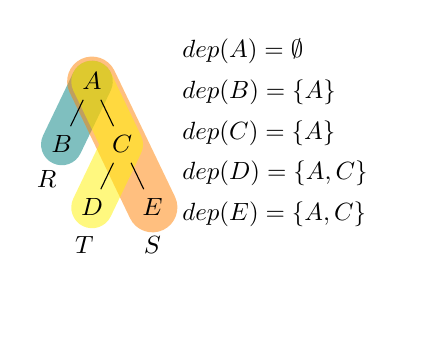
\begin{tikzpicture}[xscale=0.96, yscale=0.8]
        \node at (0, 0.0) (A) {\small  $A$};
        \node at (-0.4, -1.0) (B) {\small $B$}  edge[-] (A);
        \node at (0.4, -1.0) (C) {\small $C$} edge[-] (A);
        \node at (0.8, -2.0) (E) {\small $E$} edge[-] (C);
        \node at (0, -2.0) (D) {\small $D$} edge[-] (C);
        \node at (0.8, -2.6) (S) {\small $S$};
        \node at (-0.6, -1.55) (R) {\small  $R$};
        \node at (-0.1, -2.6) (T) {\small  $T$};
                \node at (2.3, -1.5) {\scalebox{0.9} {
        \begin{tabular}{@{~~~~}l}
          $dep(A) = \emptyset$\\[1ex]
          $dep(B)=\{A\}$\\[1ex]
          $dep(C)=\{A\}$\\[1ex]
          $dep(D)=\{A,C\}$\\[1ex]
          $dep(E)=\{A,C\}$\\[8ex]
        \end{tabular}
      }};
        \begin{pgfonlayer}{background}
          \draw[opacity=.5,fill opacity=.5,line cap=round, line join=round, line width=15pt,color=teal] (0,0.0) -- (-0.4,-1);
          \draw[opacity=.5,fill opacity=.5,line cap=round, line join=round, line width=18pt,color=orange] (0,0.0) -- (0.8,-2.0);
          \draw[opacity=.5,fill opacity=.5,line cap=round, line join=round, line width=15pt,color=yellow] (0,0.0) -- (0.4,-1) -- (0, -2.0);
        \end{pgfonlayer}
      \end{tikzpicture}
      % }
    \end{minipage}
  \hspace{1.2cm}
    \begin{minipage}[b]{0.4\linewidth}
    % \scalebox{0.9}{
  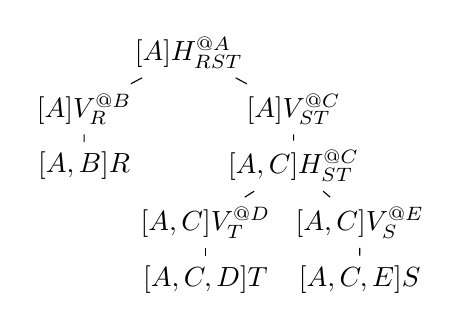
\begin{tikzpicture}[xscale=0.7, yscale=0.24]

    \node at (-0.4, 3) (A) {$\VIEW[A]{H^{@A}_{RST}}$};     
     \node at (1.5, 0) (C) {$\VIEW[A]{V^{@C}_{ST}}$} edge[-] (A);      
     \node at (1.5, -3) (C') {$\VIEW[A,C]{H^{@C}_{ST}}$} edge[-] (C);      
     \node at (2.7, -6) (E) {$\VIEW[A,C]{V^{@E}_{S}}$} edge[-] (C');
      \node at (2.7, -9) {$\VIEW[A,C,E]{S}$} edge[-] (E);
    
    \node at (-0.1, -6) (D) {$\VIEW[A,C]{V^{@D}_{T}}$} edge[-] (C');
      \node at (-0.1, -9) {$\VIEW[A,C,D]{T}$} edge[-] (D);  

      \node at (-2.3, -0) (B) {$\VIEW[A]{V^{@B}_{R}}$} edge[-] (A);
      \node at (-2.3, -3) {$\VIEW[A,B]{R}$} edge[-] (B);  
    \end{tikzpicture}
% }
    \end{minipage}
    \caption{(left) Canonical free-top variable order of the query $\VIEW[]{Q_h}$ from Example 
    \ref{ex:hierarchical}; 
    (right) Corresponding view tree.}
    \label{fig:q-hierarchical_view_tree}
    \end{figure}
    
\begin{example}
\label{ex:hierarchical}
The free-connex acyclic query 
$\VIEW[A,B,C]{Q}$ $=$ 
$\VSUM_{D}\VSUM_{E}$ $\VIEW[A,B]{R} \VPROD \VIEW[A,C,E]{S} \VPROD \VIEW[C,D]{T}$
from Example~\ref{ex:acyclic} is not hierarchical: the sets $\textsf{rels}(A)= \{\VIEW[]{R} , \VIEW[]{S}\}$
$\textsf{rels}(C)= \{\VIEW[]{S} , \VIEW[]{T}\}$ are not disjoint, nor one is included in the other.
By extending the schema of $\VIEW[]{T}$ with $A$, we obtain the $q$-hierarchical query 
$\VIEW[A,B,C]{Q_h}$ $=$ 
$\VSUM_{D}\VSUM_{E}$ $\VIEW[A,B]{R} \VPROD \VIEW[A,C,E]{S} \VPROD \VIEW[A,C,D]{T}$
whose canonical free-top variable order is given in Figure~\ref{fig:q-hierarchical_view_tree} (left).
The variant of the query,  
where variable $A$ is bound is hierarchical but not $q$-hierarchical because  
the set $\mathsf{rels}(A)= \{\VIEW[]{R}, \VIEW[]{S}, \VIEW[]{T}\}$ 
for the  \emph{bound} variable  $A$ is a strict superset of the set 
$\mathsf{rels}(B)= \{\VIEW[]{R}\}$ for the \emph{free} variable $B$.
\punto
\end{example}
     
We next exemplify  how \DF achieves constant-time update for a $q$-hierarchical query.       
   
\begin{example}\label{ex:qhierarchical-update}
Figure~\ref{fig:q-hierarchical_view_tree} shows the view tree (right)
modeled on the canonical free-top variable order (left) of the 
$q$-hierarchical query $\VIEW[]{Q_h}$ in Example~\ref{ex:hierarchical}.
Figure~\ref{fig:q-hierarchical_delta_view_trees} shows the
delta view trees under single-tuple updates to $\VIEW[]{R}$  and $\VIEW[]{T}$.

In the delta view tree for $\VIEW[]{R}$, the delta view
$\delta \VIEW[]{H^{@A}_{RST}}$ can be computed by  a constant-time lookup in 
$\VIEW[]{V^{@C}_{ST}}$.   
In the delta view tree for $\VIEW[]{T}$, the delta views
$\delta \VIEW[]{H^{@C}_{ST}}$ and $\delta \VIEW[]{H^{@A}_{RST}}$ 
can be computed by constant-time lookups in 
$\VIEW[]{V^{@E}_{S}}$ and $\VIEW[]{V^{@B}_{R}}$, respectively. 
All other delta views are computed by marginalizing a variable with a single value. 
\punto
\end{example}

\begin{figure}[t]
    \hspace{-0.15cm}
    \centering
    \begin{minipage}[b]{0.3\linewidth}
    % \scalebox{0.87}{
  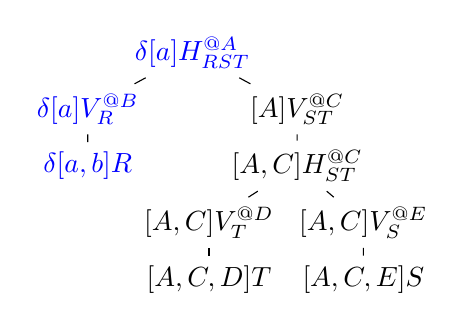
\begin{tikzpicture}[xscale=0.7, yscale=0.24]

    \node at (-0.4, 3) (A) {$\color{blue} \delta \VIEW[a]{H^{@A}_{RST}}$};     
     \node at (1.5, 0) (C) {$\VIEW[A]{V^{@C}_{ST}}$} edge[-] (A);      
     \node at (1.5, -3) (C') {$\VIEW[A,C]{H^{@C}_{ST}}$} edge[-] (C);      
     \node at (2.7, -6) (E) {$\VIEW[A,C]{V^{@E}_{S}}$} edge[-] (C');
      \node at (2.7, -9) {$\VIEW[A,C,E]{S}$} edge[-] (E);
    
    \node at (-0.1, -6) (D) {$\VIEW[A,C]{V^{@D}_{T}}$} edge[-] (C');
    \node at (-0.1, -9) {$\VIEW[A,C,D]{T}$} edge[-] (D);  

      \node at (-2.3, -0) (B) {$\color{blue}\delta \VIEW[a]{V^{@B}_{R}}$} edge[-] (A);
      \node at (-2.3, -3) {$\color{blue}\delta \VIEW[a,b]{R}$} edge[-] (B);  
\end{tikzpicture}
% }
    \end{minipage}
  \hspace{1.5cm}
    \begin{minipage}[b]{0.4\linewidth}
    % \scalebox{0.87}{
  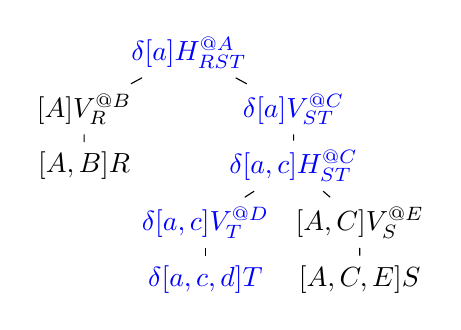
\begin{tikzpicture}[xscale=0.7, yscale=0.24]

    \node at (-0.4, 3) (A) {$\color{blue} \delta \VIEW[a]{H^{@A}_{RST}}$};     
     \node at (1.5, 0) (C) {$\color{blue}\delta \VIEW[a]{V^{@C}_{ST}}$} edge[-] (A);      
     \node at (1.5, -3) (C') {\color{blue}$\delta \VIEW[a,c]{H^{@C}_{ST}}$} edge[-] (C);      
     \node at (2.7, -6) (E) {$\VIEW[A,C]{V^{@E}_{S}}$} edge[-] (C');
      \node at (2.7, -9) {$\VIEW[A,C,E]{S}$} edge[-] (E);
    
    \node at (-0.1, -6) (D) {$\color{blue}\delta \VIEW[a,c]{V^{@D}_{T}}$} edge[-] (C');
    \node at (-0.1, -9) {$\color{blue}\delta \VIEW[a,c,d]{T}$} edge[-] (D);  

    \node at (-2.3, -0) (B) {$\VIEW[A]{V^{@B}_{R}}$} edge[-] (A);
    \node at (-2.3, -3) {$\VIEW[A,B]{R}$} edge[-] (B);  
\end{tikzpicture}
% }
    \end{minipage}
    \caption{Delta view trees derived from the view tree in Figure~\ref{fig:q-hierarchical_view_tree} 
for single-tuple updates to relations $\VIEW[]{R}$ (left) and $\VIEW[]{T}$ (right).}
    \label{fig:q-hierarchical_delta_view_trees}
    \end{figure}
 
\begin{remark}
  $Q$-hierarchical queries admit view trees who\-se views only need primary indices to support payload lookup and updates and possibly secondary indices to support enumeration.
  Consider the view tree in Figure~\ref{fig:q-hierarchical_view_tree}. Enumeration proceeds top-down: We iterate over the $A$-values in the top view and for each such value $a$, 
  %we look up in $\VIEW[a]{V^{@B}_{R}}$ and $\VIEW[a]{V^{@C}_{ST}}$, then continue to 
  we look up in $\VIEW[a,B]{R}$ to enumerate over all the $B$-values paired with $a$, and also look up into $\VIEW[a,C]{H^{@C}_{ST}}$ to enumerate over all $C$-values paired with $a$. %We continue similarly to get all $D$-values and $E$-values paired with $a$ and each $C$-value. 
  All these look-ups require primary or secondary indices.  
  
  
  Figure~\ref{fig:q-hierarchical_delta_view_trees} shows the delta view trees for single-tuple updates to $\VIEW[]{R}$ and $\VIEW[]{T}$. To compute a delta view along the path from the delta relation to the root of the delta view tree, we either perform a projection on a delta view or a lookup in the primary index of a sibling view (so with all keys of the index set to constants).\punto
\end{remark}

%%%%%%%%%%%%%%%%%%%%%%%%%%%%%%%%%
\subsection{Queries under Functional Dependencies}

Non-hierar\-chical queries may become hierarchical under functional dependencies (fds)~\cite{OlteanuHK09}.

Given a set $\Sigma$ of fds, we denote by $\textsf{CLOSURE}_\Sigma(\calS)$ the closure of the set $\calS$ of variables under $\Sigma$~\cite{AbiteboulHV95}. For instance, given the fds $\Sigma=\{A\rightarrow D;BD \rightarrow E\}$, we have $\textsf{CLOSURE}_\Sigma(\{A,B,C\})=\{A,B,C,D,E\}$.

\begin{definition}[adapted from~\cite{OlteanuHK09}]
  Given a set $\Sigma$ of fds and a query $\VIEW[\calS]{Q} = \VSUM_{\calB} \VIEW[\calS_1]{R_1}\VPROD\cdots\VPROD\VIEW[\calS_n]{R_n}$, the \emph{$\Sigma$-reduct} of $\VIEW[]{Q}$ under $\Sigma$ is:
\begin{align*}
  \;
  \VIEW[\textsf{CLOSURE}_\Sigma(\calS)]{Q} = \VSUM_{\calB} &\VIEW[\textsf{CLOSURE}_\Sigma(\calS_1)]{R_1}\VPROD\cdots\VPROD \VIEW[\textsf{CLOSURE}_\Sigma(\calS_n)]{R_n}
\end{align*}
\end{definition}
The $\Sigma$-reduct of a query is thus another query, where the schema of each relation is extended to include all variables in the closure of this schema under $\Sigma$. Since the added variables are functionally determined by the original schema, they do not add more information. So, we could extend these schemas and the underlying database without increasing the number of tuples in the relations. For any database $D$ with fds $\Sigma$ and a query $\VIEW[]{Q}$, the query result $\VIEW[]{Q}(D)$ is the same as the result of its $\Sigma$-reduct over the extended database.
The benefit of this rewriting is that queries may admit free-connex acyclic or even $q$-hierarchical $\Sigma$-reducts. We need not physically extend the database to reap this benefit. Instead, we use the $\Sigma$-reduct of $\VIEW[]{Q}$ to infer a free-top variable order or even a canonical free-top variable order \emph{for} $\VIEW[]{Q}$ in case the $\Sigma$-reduct is free-connex acyclic or $q$-hierarchical, respectively.
Using this variable order, we construct a view tree for $\VIEW[]{Q}$ that enjoys the preprocessing, update, and enumerate times as for its $\Sigma$-reduct.

Theorem~\ref{th:special-cases} can be generalized to account for fds.

\begin{theorem}\label{th:special-cases-fds}
  Let a query $\VIEW[]{Q}$ and a database of size $N$ and with a set $\Sigma$ of functional dependencies.

  \DF can maintain $\VIEW[]{Q}$ with $O(N)$ preprocessing, $O(1)$ enumeration delay, and $O(N)$ single-tuple updates in case the $\Sigma$-reduct of $\VIEW[]{Q}$ is free-connex acyclic.
    
  \DF can maintain $\VIEW[]{Q}$ with $O(N)$ preprocessing, $O(1)$ enumeration delay, and $O(1)$ single-tuple updates in case the $\Sigma$-reduct of $\VIEW[]{Q}$ is $q$-hierarchical.
\end{theorem}

  \begin{figure}[t]
   \hspace{-0.1cm}
   \centering
    \begin{minipage}[b]{0.2\linewidth}
    % \scalebox{0.88}{
      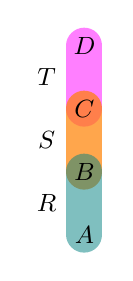
\begin{tikzpicture}[xscale=0.96, yscale=0.8]
        \node at (0, 0) (D) {\small  $D$};
        \node at (0, -1) (C) {\small $C$};
        \node at (0, -2) (B) {\small $B$};
        \node at (0, -3) (A) {\small $A$};
        
    \node at (-0.5, -0.5) (T) {\small  $\VIEW{T}$};    
        \node at (-0.5, -1.5) (S) {\small  $\VIEW{S}$};    
            \node at (-0.5, -2.5) (R) {\small  $\VIEW{R}$};    
\begin{pgfonlayer}{background}
\draw[opacity=.5,fill opacity=.5,line cap=round, line join=round, line width=13pt,color=purple] (0,0) -- (0,-1);\draw[opacity=0.7,fill opacity=0.7,line cap=round, line join=round, line width=13pt,color=orange] (0,-1) -- (0,-2.0);
\draw[opacity=.5,fill opacity=.5,line cap=round, line join=round, line width=13pt,color=teal] (0,-2) -- (0,-3);
        \end{pgfonlayer}
      \end{tikzpicture}
      % }
    \end{minipage}
  \hspace{-0.5cm}
\begin{minipage}[b]{0.2\linewidth}
    % \scalebox{0.88}{
      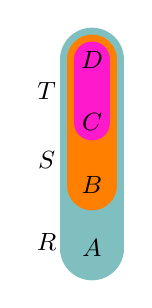
\begin{tikzpicture}[xscale=0.96, yscale=0.8]
        \node at (0, 0) (D) {\small  $D$};
        \node at (0, -1) (C) {\small $C$};
        \node at (0, -2) (B) {\small $B$};
        \node at (0, -3) (A) {\small $A$};
        
            \node at (-0.6, -0.5) (T) {\small  $\VIEW{T}$};    
        \node at (-0.6, -1.6) (S) {\small  $\VIEW{S}$};    
            \node at (-0.6, -2.9) (R) {\small  $\VIEW{R}$};    
\begin{pgfonlayer}{background}
\draw[opacity=.5,fill opacity=1,line cap=round, line join=round, line width=23pt,color=teal] (0,0) -- (0,-3);
\draw[opacity=1,fill opacity=1,line cap=round, line join=round, line width=18pt,color=orange] (0,0) -- (0,-2);
\draw[opacity=0.8,fill opacity=0.8,line cap=round, line join=round, line width=13pt,color=purple] (0,0) -- (0,-1);
        \end{pgfonlayer}
      \end{tikzpicture}
      % }
    \end{minipage}    
    \hspace{-0.2cm}
    \begin{minipage}[b]{0.3\linewidth}
    % \scalebox{0.88}{
      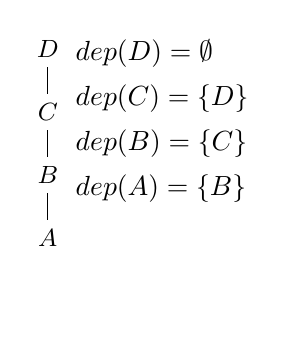
\begin{tikzpicture}[xscale=0.96, yscale=0.8]
        \node at (0, 0) (D) {\small  $D$};
        \node at (0, -1) (C) {\small $C$}edge[-] (D);
        \node at (0, -2) (B) {\small $B$}edge[-] (C);
        \node at (0, -3) (A) {\small $A$}edge[-] (B);
                   \node at (1.5, -1.9) {
        \begin{tabular}{@{~~}l}
          $dep(D)=\emptyset$\\[1ex]
          $dep(C)=\{D\}$\\[1ex]
          $dep(B)=\{C\}$\\[1ex]
          $dep(A)=\{B\}$\\[8ex]
        \end{tabular}
      }; 
      \end{tikzpicture}
      % }
      % \vspace{-0.2cm}
    \end{minipage}
    \hspace{0cm}
    \begin{minipage}[b]{0.2\linewidth}
    \scalebox{0.88}{
  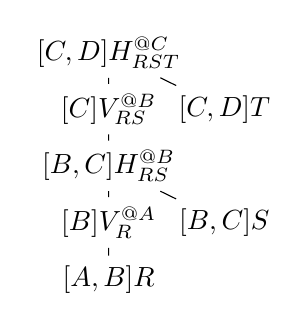
\begin{tikzpicture}[xscale=0.7, yscale=0.24]    
      \node at (-2.3, 6) (C) {$\VIEW[C,D]{H^{@C}_{RST}}$};
      \node at (-2.3, 3) (B) {$\VIEW[C]{V^{@B}_{RS}}$}edge[-] (C);
      \node at (-2.3, 0) (B') {$\VIEW[B,C]{H^{@B}_{RS}}$} edge[-] (B);
      \node at (-2.3, -3) (A) {$\VIEW[B]{V^{@A}_{R}}$}edge[-] (B');
      \node at (-2.3, -6) {$\VIEW[A,B]{R}$} edge[-] (A);  
      
            \node at (-0.2, -3) (S) {$\VIEW[B,C]{S}$}edge[-] (B');
      \node at (-0.2, 3) (T) {$\VIEW[C,D]{T}$}edge[-] (C);
\end{tikzpicture}
}
    \end{minipage}
    \caption{From left to right: Hypergraph of the query 
    $\VIEW{Q}$ and its $\Sigma$-reduct for $\Sigma = \{B \rightarrow C, C \rightarrow D\}$
    from Example~\ref{ex:q_hierarchical_rewriting}; 
    canonical variable order $\omega$ for  $\VIEW{Q}$; view tree modeled on $\omega$.}
    \label{fig:q-hierarchical_rewriting} 
    \end{figure}

%%%%%%%%%%%%%%%
    
  \begin{figure}[t]
 \hspace{-0.2cm}
 \centering
    \begin{minipage}[b]{0.2\linewidth}
    % \scalebox{0.93}{
  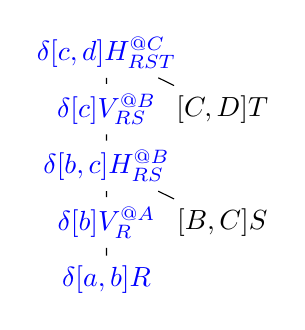
\begin{tikzpicture}[xscale=0.7, yscale=0.24]    
      \node at (-2.3, 6) (C) {\color{blue}$\delta\VIEW[c,d]{H^{@C}_{RST}}$};
      \node at (-2.3, 3) (B) {\color{blue}$\delta\VIEW[c]{V^{@B}_{RS}}$}edge[-] (C);
      \node at (-2.3, 0) (B') {$\color{blue}\delta\VIEW[b,c]{H^{@B}_{RS}}$} edge[-] (B);
      \node at (-2.3, -3) (A) {$\color{blue}\delta\VIEW[b]{V^{@A}_{R}}$}edge[-] (B');
      \node at (-2.3, -6) {$\color{blue}\delta\VIEW[a,b]{R}$} edge[-] (A);  
      
            \node at (-0.2, -3) (S) {$\VIEW[B,C]{S}$}edge[-] (B');
      \node at (-0.2, 3) (T) {$\VIEW[C,D]{T}$}edge[-] (C);
\end{tikzpicture}
% }
    \end{minipage}
    \hspace{1cm}
    \begin{minipage}[b]{0.2\linewidth}
    % \scalebox{0.93}{
  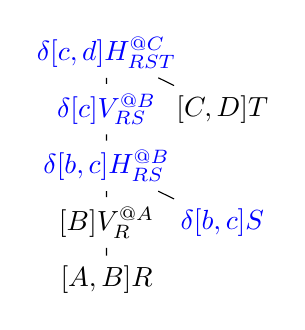
\begin{tikzpicture}[xscale=0.7, yscale=0.24]    
      \node at (-2.3, 6) (C) {\color{blue} $\delta\VIEW[c,d]{H^{@C}_{RST}}$};
      \node at (-2.3, 3) (B) {\color{blue}$\delta\VIEW[c]{V^{@B}_{RS}}$}edge[-] (C);
      \node at (-2.3, 0) (B') {\color{blue}$\delta\VIEW[b,c]{H^{@B}_{RS}}$} edge[-] (B);
      \node at (-2.3, -3) (A) {$\VIEW[B]{V^{@A}_{R}}$}edge[-] (B');
      \node at (-2.3, -6) {$\VIEW[A,B]{R}$} edge[-] (A);  
      
            \node at (-0.2, -3) (S) {\color{blue}$\delta\VIEW[b,c]{S}$}edge[-] (B');
      \node at (-0.2, 3) (T) {$\VIEW[C,D]{T}$}edge[-] (C);
\end{tikzpicture}
% }
    \end{minipage}
    \hspace{1cm}
    \begin{minipage}[b]{0.2\linewidth}
    % \scalebox{0.93}{
  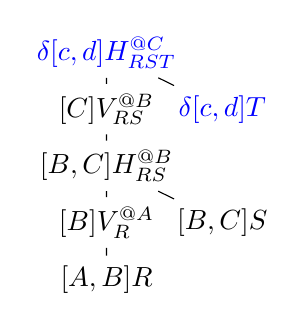
\begin{tikzpicture}[xscale=0.7, yscale=0.24]    
      \node at (-2.3, 6) (C) {\color{blue}$\delta\VIEW[c,d]{H^{@C}_{RST}}$};
      \node at (-2.3, 3) (B) {$\VIEW[C]{V^{@B}_{RS}}$}edge[-] (C);
      \node at (-2.3, 0) (B') {$\VIEW[B,C]{H^{@B}_{RS}}$} edge[-] (B);
      \node at (-2.3, -3) (A) {$\VIEW[B]{V^{@A}_{R}}$}edge[-] (B');
      \node at (-2.3, -6) {$\VIEW[A,B]{R}$} edge[-] (A);  
      
            \node at (-0.2, -3) (S) {$\VIEW[B,C]{S}$}edge[-] (B');
      \node at (-0.2, 3) (T) {\color{blue}$\delta\VIEW[c,d]{T}$}edge[-] (C);
\end{tikzpicture}
% }
    \end{minipage}
    \caption{Delta view trees derived from the view tree in Figure~\ref{fig:q-hierarchical_rewriting} for single-tuple updates to 
% $\VIEW{R}$ (left), $\VIEW{S}$ (middle), and $\VIEW{T}$ (right). 
$\VIEW{R}$, $\VIEW{S}$, and $\VIEW{T}$ (left to right). 
The values $b$ and $c$ functionally determine $c$ and $d$, respectively.}
    \label{fig:q-hierarchical_rewriting_delta}
    \end{figure}
    
\begin{example} 
\label{ex:q_hierarchical_rewriting}
Consider $\Sigma = \{B \rightarrow C, C \rightarrow D\}$ and the free-connex acyclic but not hierarchical query
\begin{align*}
\quad  \VIEW[A,B,C,D]{Q} =\VIEW[A,B]{R} \VPROD \VIEW[B,C]{S} \VPROD \VIEW[C,D]{T}.
\end{align*}
The $\Sigma$-reduct of $\VIEW[]{Q}$ is 
\begin{align*}
\VIEW[A,B,C,D]{Q'} \hspace{-0.1em} =\VIEW[A,B,C,D]{R} \VPROD \VIEW[B,C,D]{S} \VPROD \VIEW[C,D]{T}.
\end{align*}
Figure~\ref{fig:q-hierarchical_rewriting} depicts the hypergraphs
of $\VIEW[]{Q}$ and $\VIEW[]{Q'}$ (left), a free-top variable order for 
$\VIEW[]{Q}$ that is also canonical for $\VIEW[]{Q'}$ (middle), and 
the view tree for $\VIEW[]{Q}$ modeled on this variable order (right).
Since $\VIEW{Q}$ is free-connex acylic, we can compute the view tree in linear time and enumerate the result tuples of $\VIEW{Q}$ with constant delay, as explained in Section~\ref{sec:free-connex}. 
We next describe how to achieve constant-time update by exploiting 
  the fds. Figure~\ref{fig:q-hierarchical_rewriting_delta} shows the delta view trees obtained from the view tree for $\VIEW{Q}$ for single-tuple updates to $\VIEW{R}$, $\VIEW{S}$, and $\VIEW{T}$.

Consider first the update $\delta\VIEW[a,b]{R}$ to relation $\VIEW[]{R}$. The delta view $\delta\VIEW[b]{V^{@A}_{R}}$ is just a projection of the update tuple. The delta view $\delta\VIEW[b,c]{H^{@B}_{RS}}$ requires a lookup in $\VIEW[B,C]{S}$ for $B=b$. In general, there may be many $C$-values paired with $b$. However, under the fd $B\rightarrow C$, there is at most one $C$-value $c$ paired with $b$. Hence, the construction of this delta view takes constant time. Similarly, the delta view $\delta\VIEW[c,d]{H^{@C}_{RST}}$ requires a lookup in $\VIEW[C,D]{T}$ for $C=c$. Again, there may be many $D$-values paired with $c$, yet under the fd $C\rightarrow D$, there is at most one $D$-value $d$ paired with $c$. Hence, the construction of this delta view takes constant time, too.

Similar reasoning applies to the update $\delta\VIEW[b,c]{S}$. To compute the delta view $\delta\VIEW[c,b]{H^{@B}_{RS}}$, we need a constant-time lookup in the view $\VIEW[B]{V^{@A}_R}$ with $B=b$. Computing $\delta\VIEW[c,d]{H^{@C}_{RST}}$ takes constant time due to the fd $C\rightarrow D$, as with updates to  $\VIEW{R}$. 
Processing the update $\delta\VIEW[c,d]{T}$ takes constant time without exploiting the fds: it only requires a lookup in the view $\VIEW[C]{V^{@B}_{RS}}$ with $C=c$. \punto
\end{example} 
%%%%%%%%%%%%%%%%%%%%%%%%%%%%%%%%%%%%
%!TEX root = main.tex
\add{
\subsection{Cyclic Queries}
\label{sec:cyclic_queries}
Our framework supports arbitrary conjunctive queries. Whereas for an acyclic join query the size of each view is asymptotically upper-bounded by the size of the query result, for a cyclic query views may be larger in size than the 
query result. 
%This increase in space may however enable faster view maintenance.
In prior work~\cite{FIVM:SIGMOD:2018}, we show how to reduce the size of intermediate views
for cyclic queries  by extending view trees with indicator projections~\cite{FAQ:PODS:2016}.  Such projections have no effect on the query result but can constrain view definitions (e.g., create cycles) and bring asymptotic savings in space and time. 

}

\begin{example}\label{ex:triangle_query_ivm}
We consider the triangle query: 
%over the ring $\mathbb{Z}$:
% 
$$
\VIEW[~]{Q_{\vartriangle}} = \VSUM_{A}\VSUM_{B}\VSUM_{C} \VIEW[A,B]{R} \VPROD \VIEW[B,C]{S} \VPROD \VIEW[C,A]{T} 
$$

Figure~\ref{fig:triangle_hypergraph_viewtree} shows the hypergraph of $Q_{\vartriangle}$ and the view tree constructed for the variable order $A-B-C$ by placing each relation directly under its lowest variable. We assume all {relations} are of size $\bigO{N}$. Computing the triangle query from scratch using a worst-case optimal join algorithm takes $\bigO{N^{3/2}}$ time~\cite{Ngo:SIGREC:2013}.

In the given view tree (without the view in red), we first join $\VIEW{S}$ and $\VIEW{T}$ and then marginalize out $C$.
This view at node $C$ may contain $\bigO{N^2}$ pairs of $(A,B)$ values, which is larger than the worst-case size $\bigO{N^{3/2}}$. 
However, by materializing the view at $C$, we enable single-tuple updates to $R$ in constant time; single-tuple updates to other relations take $\bigO{N}$ time.

To avoid the large intermediate result at variable $C$, we can change the view tree by placing the relation $R$ under variable $C$. Then, joining all three relations at node $C$ takes $\bigO{N^{3/2}}$ time. Updates to any relation now cause recomputation of a $3$-way join, like in first-order IVM. For single-tuple updates, recomputing deltas takes $\bigO{N}$ as only two of the three variables are bound to constants. In contrast, the first approach trades off space for time: We need $\bigO{N^2}$ space but then support $\bigO{1}$ updates to one of the three relations.
\punto
\end{example}


\begin{figure}\centering
  \begin{tabular}[c]{l@{~~~}l}  
    \begin{minipage}[b]{3cm}
      \scalebox{0.9}{
      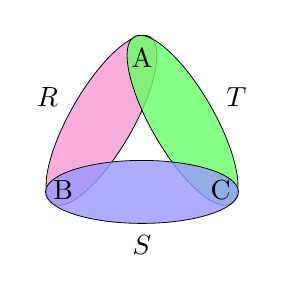
\begin{tikzpicture}[scale=0.5]
        \node at (-2.4, -2) (r) {$R$};
        \node at (2.4, -2) (r) {$T$};
        \node at (0, -5.75) (r) {$S$};
        \draw[rotate=60,line width=0.1mm,fill opacity=0.8,fill=magenta!40] (-2.75,-0.4) ellipse (2.45cm and 0.8cm);
       \draw[rotate=-60,line width=0.1mm,fill opacity=0.8,fill=green!60] (2.75,-0.4) ellipse (2.45cm and 0.8cm);
        \draw[rotate=0,line width=0.1mm,fill opacity=0.8,fill=blue!40] (0,-4.4) ellipse (2.45cm and 0.8cm);
        \node at (0, -1) (A) {A};
        \node at (-2, -4.35) (B) {B};
        \node at (2, -4.35) (C) {C};
      \end{tikzpicture}
      }
      \vspace{2mm}
    \end{minipage}
    &
    \begin{minipage}[b]{5cm}
      \scalebox{0.9}{
      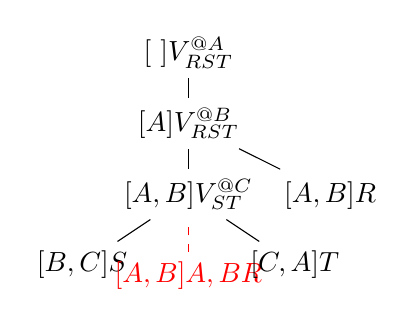
\begin{tikzpicture}[xscale=0.9,yscale=0.9]
        \node at (0, 0) (A) {$\VIEW[~]{V^{@A}_{RST}}$};
        \node at (0, -1) (B) {$\VIEW[A]{V^{@B}_{RST}}$} edge[-] (A);
        \node at (0, -2) (C) {$\VIEW[A,B]{V^{@C}_{ST}}$} edge[-] (B);

        \node at (2, -2) (R) {$\VIEW[A,B]{R} \makebox[0pt][l]{$\phantom{\VIEW[A,B]{V^{@C}}}$} $} edge[-] (B);
        \node at (-1.5, -3) (S) {$\VIEW[B,C]{S}$} edge[-] (C);
        \node[color=red] at (-0, -3.15) (S) {$\VIEW[A,B]{\displaystyle\VEXISTS{A,B}{R}}$} edge[red,dashed] (C);
        \node at (1.5, -3) (T) {$\VIEW[C,A]{T}$} edge[-] (C);
      \end{tikzpicture}
  }    
    \end{minipage}
    \end{tabular}
    % \vspace*{-1em}
\caption{(left) Hypergraph of the triangle query $Q_{\vartriangle}$; (right) View tree for the variable order $A - B - C$ with an indicator projection $\exists_{A,B}\VIEW{R}$.}
\label{fig:triangle_hypergraph_viewtree}
% \vspace*{2em}
\end{figure}


\nop{
\begin{figure}\centering
  \begin{tabular}[c]{@{}l@{~}l@{}}  
    \begin{minipage}[b]{2.3cm}
      \hspace*{-4mm}
      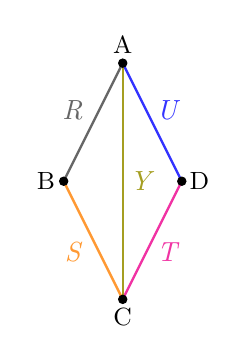
\begin{tikzpicture}[xscale=0.75,yscale=0.75]

        \draw[thick,darkgray!80,line width=0.3mm] (0,0) -- (-1,-2);
        \draw[thick,blue!80,line width=0.3mm] (0,0) -- (1,-2);        
        \draw[thick,orange!80,line width=0.3mm] (-1,-2) -- (0,-4);
        \draw[thick,magenta!80,line width=0.3mm] (1,-2) -- (0,-4);
        \draw[thick,olive!80,line width=0.3mm] (0,0) -- (0,-4);

        \draw[fill=black] (0,0) circle (0.7mm);
        \draw[fill=black] (-1,-2) circle (0.7mm);
        \draw[fill=black] (1,-2) circle (0.7mm);
        \draw[fill=black] (0,-4) circle (0.7mm);

        \node at (0,0.3) {\small A};
        \node at (-1.3,-2) {\small B};        
        \node at (1.3,-2) {\small D};
        \node at (0.0,-4.3) {\small C};

        \node at (-0.85, -0.8) (r) {\color{darkgray!80}\it R};
        \node at (0.75, -0.8) (r) {\color{blue!80}\it U};
        \node at (-0.85, -3.2) (r) {\color{orange!80}\it S};
        \node at (0.75, -3.2) (r) {\color{magenta!80}\it T};
        \node at (0.3, -2) (r) {\color{olive!80}\it Y};
      \end{tikzpicture}
      \vspace{3mm}
    \end{minipage}
    &
    \begin{minipage}[b]{5.5cm}
      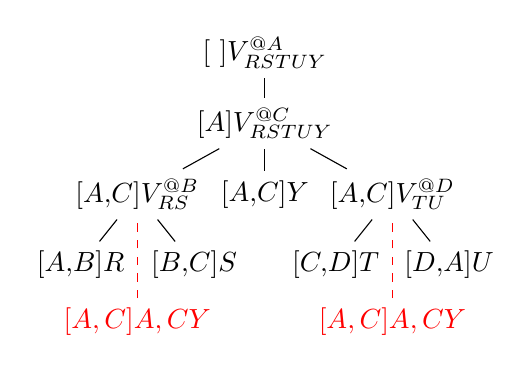
\begin{tikzpicture}[xscale=0.9,yscale=0.9]
        \node at (0, 0) (A) {$\VIEW[~]{V^{@A}_{RSTUY}}$};
        \node at (0, -1) (C) {$\VIEW[A]{V^{@C}_{RSTUY}}$} edge[-] (A);
        \node at (-1.8, -2) (B) {$\VIEW[A,\!C]{V^{@B}_{RS}}$} edge[-] (C);
        \node at (0, -2) (Y) {$\VIEW[A,\!C]{Y}$} edge[-] (C);
        \node at (1.8, -2) (D) {$\VIEW[A,\!C]{V^{@D}_{TU}}$} edge[-] (C);
        \node at (-2.6, -3) (R) {$\VIEW[A,\!B]{R}$} edge[-] (B);
        \node at (-1.0, -3) (S) {$\VIEW[B,\!C]{S}$} edge[-] (B);
        \node at (1.0, -3) (T) {$\VIEW[C,\!D]{T}$} edge[-] (D);
        \node at (2.6, -3) (U) {$\VIEW[D,\!A]{U}$} edge[-] (D);

        \node[color=red] at (-1.8, -3.8) (P1) {$\VIEW[A,C]{\VEXISTS{A,C}Y}$} edge[red,dashed] (B);
        \node[color=red] at (1.8, -3.8) (P2) {$\VIEW[A,C]{\VEXISTS{A,C}Y}$} edge[red,dashed] (D);
      \end{tikzpicture}
    \end{minipage}
    \end{tabular}
\caption{\label{fig:cyclic_hypergraph_viewtree}(left) Hypergraph of the cyclic query $Q_{\boxslash}$; (right) View tree for the variable order $A - C - \{ B, D \}$ with indicator projections (in red).}
\vspace{-1em}
\end{figure}
}

The above example demonstrates how placing a relation under a different node in a view tree can create a cycle of relations and constrain the size of a view. This strategy, however, might not be always feasible or efficient: One relation might form multiple cycles of relations in different parts of a view tree -- for example, in the cyclic $4$-loop
 query $\VIEW[~]{Q_{\boxslash}}$ $=$ 
 $\VSUM_{A}\VSUM_{B}\VSUM_{C} \VSUM_{D}$ $\VIEW[A,B]{R}\VPROD \VIEW[B,C]{S} \VPROD \VIEW[C,D]{T}
 \VPROD \VIEW[D,A]{U} \VPROD \VIEW[A,C]{W}$ the chord relation $\VIEW{W}$ is part of two triangle subqueries. Since this relation cannot be duplicated in multiple subtrees (for correctness reasons so as to avoid multiplying the same payload several times instead of using it once), one would have to evaluate these subqueries in sequence, which yields a view tree that is higher and more expensive to maintain. 

\paragraph{\textbf{Indicator Projections.}}
Instead of moving relations in a view tree, we extend the tree with indicator projections that identify the active domains of these relations~\cite{FAQ:PODS:2016}. Such projections have no effect on the query result but can constrain view definitions (e.g., create cycles) and bring asymptotic savings in space and time. 

We define a new unary operation $\VEXISTS{\mathcal{A}}{\VIEW{R}}$ that, given a relation $\VIEW{R}$ over schema 
$\mathcal{S}$ with payloads from a ring $(\RING, \RINGPLUS, \RINGPROD, \RINGZERO, \RINGONE)$, and a set of attributes $\mathcal{A} \subseteq \mathcal{S}$, projects tuples from $\VIEW{R}$ with non-$\RINGZERO$ payload on $\mathcal{A}$ and assigns to these tuples the payload $\RINGONE$. 


\begin{definition}[Indicator Projection]
   For a relation R over schema $\calS$ and $\calA \subseteq \calS$, 
   the indicator projection $\VEXISTS{\mathcal{A}}{\VIEW{R}}$ is a relation over $\calA$ such that
   $\forall \vecnormal{t} \in \Dom(\calA)$:
\begin{align*}
  \left( \textstyle\VEXISTS{\mathcal{A}}{\VIEW{R}} \right)[\vecnormal{t}] = 
  \begin{cases} 
    \RINGONE & \exists\vecnormal{s} \in\Dom(\mathcal{S}), \vecnormal{s}\in \VIEW{R}, \vecnormal{t} = \pi_{\mathcal{A}}(\vecnormal{s})\\
    \RINGZERO & \text{otherwise}
  \end{cases}
\end{align*}
\end{definition}


\nop{
The delta rule for $\VEXISTS{\mathcal{A}}$ is $\delta(\VEXISTS{\mathcal{A}}{\VIEW{R}}) = \VEXISTS{\mathcal{A}}(\VIEW{R} + \delta{\VIEW{R}}) - \VEXISTS{\mathcal{A}}{\VIEW{R}}$. This rule recomputes the query twice, once to insert new contents and once to delete the old contents, which clearly defeats the purpose of incremental computation. Note that some tuples might be unaffected by a given update $\delta{\VIEW{R}}$, so inserting those tuples and deleting them again is wasted work.

We observe that $\delta(\VEXISTS{\mathcal{A}}{\VIEW{R}})$ might change in the output only those tuples from $\VEXISTS{\mathcal{A}}{\delta{\VIEW{R}}}$. We exploit this restriction to refine the delta rule as: $\delta(\VEXISTS{\mathcal{A}}{\VIEW{R}}) = \VEXISTS{\mathcal{A}}{\delta{\VIEW{R}}} \VPROD (\VEXISTS{\mathcal{A}}(\VIEW{R} + \delta{\VIEW{R}}) - \VEXISTS{\mathcal{A}}{\VIEW{R}})$.
}

Indicator projections may change with updates to input relations. For instance, adding a tuple with a 
new $\mathcal{A}$-value to $\VIEW{R}$ enlarges the result of $\VEXISTS{\mathcal{A}}\VIEW{R}$; similarly, deleting the last tuple with the given $\mathcal{A}$-value reduces the result. One change in the input may cause at most one change in the output: $|\delta{(\VEXISTS{\mathcal{A}}\VIEW{R})}| \le |\delta{\VIEW{R}}|$.

To facilitate the computation of $\delta{(\VEXISTS{\mathcal{A}}\VIEW{R})}$, we keep track of how many tuples with non-$\RINGZERO$ payloads project on each $\mathcal{A}$-value. For updating the payload of a tuple in $\VIEW{R}$ from $\RINGZERO$ to non-$\RINGZERO$ (or vice versa), we increase (decrease) the count corresponding to the given $\mathcal{A}$-value. If this count changes from $0$ to $1$ (meaning the $\mathcal{A}$-value is unique) or from $1$ to $0$ (meaning there are no more tuples with the $\mathcal{A}$-value), then $\delta{(\VEXISTS{\mathcal{A}}\VIEW{R})}$ contains a tuple of $\mathcal{A}$-values with the payload of $\RINGONE$ or $-\RINGONE$, respectively; otherwise, the delta is empty.

\begin{example}
Consider a relation $\VIEW{R}$ over schema $\{A,B\}$ and 
with payloads from a ring $(\RING, \RINGPLUS, \RINGPROD, \RINGZERO, \RINGONE)$. We want to maintain the result of the query $\VIEW[A]{Q} = \VEXISTS{A}\VIEW[A,B]{R}$. To compute $\VIEW[A]{\delta{Q}}$ for updates to $\VIEW{R}$ efficiently, we count the tuples from $\VIEW{R}$ with non-$\RINGZERO$ payloads for each $A$-value, denoted by $\VIEW[A]{CNT_{Q}}$. For example:
\begin{small}
\begin{align*}
  \begin{tabular}[t]{@{}l|@{~}c@{~}c@{~}c@{~}c@{}}
    $\VIEW{R}$ & A & B \\
    \midrule
    & $a_1$ & $b_1$ & $\to$ & $r_1$ \\
    & $a_1$ & $b_2$ & $\to$ & $r_2$ \\  
    & $a_2$ & $b_3$ & $\to$ & $r_3$ \\
  \end{tabular}
  \quad
  \begin{tabular}[t]{@{}l|@{~}c@{~}c@{~}c@{}}
    $\VIEW{CNT_{Q}}$ & A \\
    \midrule
    & $a_1$ & $\to$ & $2$ \\
    & $a_2$ & $\to$ & $1$ \\
  \end{tabular}
  \quad
  \begin{tabular}[t]{@{}l|@{~}c@{~}c@{~}c@{}}
    $\VIEW{Q}$ & A \\
    \midrule
    & $a_1$ & $\to$ & $\RINGONE$ \\
    & $a_2$ & $\to$ & $\RINGONE$ \\
  \end{tabular}
\end{align*}
\end{small}
where $r_1$, $r_2$, and $r_3$ are non-$\RINGZERO$ payloads from $\RING$.
% 
An update $\VIEW{\delta{R}} = \{ \tuple{a_1, b_2} \to -r_2 \}$ removes the tuple $\tuple{a_1,b_2}$ from $\VIEW{R}$, which in turn decreases $\VIEW[\text{$a_1$}]{CNT_{Q}}$ by $1$. Since there is still a tuple in $\VIEW{R}$ that projects on $a_1$, the result of $\VIEW{Q}$ remains unchanged. 
A subsequent update $\{ \tuple{a_1, b_1} \to -r_1 \}$ to $\VIEW{R}$ drops the count for $a_1$ to $0$, which triggers a change in the output, $\VIEW{\delta{Q}} = \{ \tuple{a_1} \to -\RINGONE \}$.
\punto
\end{example}


\begin{figure}[t]
	\centering
	\setlength{\tabcolsep}{3pt}
	\begin{tabular}[t]{@{}c@{}c@{}l@{}}
		\toprule
		\multicolumn{3}{c}{$indicators(\text{view tree } \tau)$ : view tree}   \\
		\midrule
		\multicolumn{3}{l}{\MATCH $\tau$:}                       \\
		\midrule
		\phantom{ab} & $\VIEW{R}(\calS))$ \hspace*{2.5em} & 

		  \RETURN $\VIEW{R}(\calS)$ \\
		\cmidrule{2-3} \\[-6pt]
		             &
		\begin{minipage}[t]{1.5cm}
			\vspace{-1.5em}
			\hspace*{-0.55cm}
			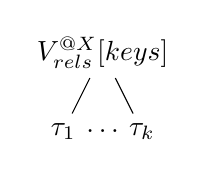
\begin{tikzpicture}[xscale=0.5, yscale=1]
				\node at (0,-2)  (n4) {$\VIEW{V_{rels}^{@X}}[keys]$};
				\node at (-1,-3)  (n1) {$\tau_1$} edge[-] (n4);
				\node at (0,-3)  (n2) {$\ldots$};
				\node at (1,-3)  (n3) {$\tau_k$} edge[-] (n4);
			\end{tikzpicture}
		\end{minipage}
		             &
		\begin{minipage}[t]{5.8cm}
			\vspace{-0.4cm}
			 \LET $\hat{\tau}_i = indicators(\tau_i)$ \ $\forall i\in[k]$ \\[0.5ex]
		          \LET $\calR $ be the set of all relation symbols  \\[0.5ex]
		           \LET $\calI = \{\VEXISTS{pk}\VIEW{R}\mid \VIEW{R} \in \calR \setminus \textsf{rels} \text{ and } \\[0.5ex]
		           \TAB\TAB\TAB\STAB pk = \sch(\VIEW{R}) \cap keys \neq \emptyset \}$ \\[0.5ex]
			 \LET $\{I_1, \ldots , I_{\ell}\} = \textsf{GYO}^*(\calI,\textsf{rels})$ \\[0.5ex] 
		  \RETURN $\left\{
				\begin{array}{@{~~}c@{~~}}
					\tikz {
						\node at (3.6,-1)  (n4) {$X$};
					        \node at (2.2,-1.75)  (n1) {$\hat{\tau}_1$} edge[-] (n4);
						\node at (2.65,-1.75)  (n2) {$\ldots$};
						\node at (3.2,-1.75)  (n3) {$\hat{\tau}_k$} edge[-] (n4);
						\node at (4.0,-1.75)  (n3) {$I_1$} edge[-] (n4);
						\node at (4.4,-1.75)  (n2) {$\ldots$};
						\node at (4.9,-1.75)  (n3) {$I_\ell$} edge[-] (n4);
					}
				\end{array}  \right.$
		\end{minipage}                                              \\[2.75ex]
		\bottomrule
	\end{tabular}
	\caption{Adding indicator projections to a view tree $\tau$. 
	Each view in $\tau$ gets as new children the indicator projections of relations that do not occur in the subtree rooted at the view  but form a cycle with those that occur. 
	$\textsf{GYO}^*$ is based on the GYO reduction~\cite{BeeriFMY83}.}
	\label{fig:indicator_projections_algo}
\end{figure}

\paragraph{\textbf{View Trees with Indicator Projections.}}
Figure~\ref{fig:indicator_projections_algo} gives an algorithm that traverses a given view tree 
recursively and extends it with indicator projections. At each view $\VIEW{V^{@X}_{rels}}$, the algorithm first computes a set 
$\calI$ of indicator projections for those relations that share common variables with $\VIEW{V^{@X}_{rels}}$ and 
do not appear in \textsf{rels}, hence do not take part 
in the view definition.
Then, it chooses from this set those indicator projections 
that form a cycle with the relations 
in the subtree rooted at $\VIEW{V^{@X}_{rels}}$. To achieve this,
it uses a variant of the \textsf{GYO} reduction~\cite{BeeriFMY83}.  
  Given the hypergraph formed by 
the hyperedges representing the indicator projections $\calI$ and the relations \textsf{rels}, 
\textsf{GYO} repeatedly applies two rules until it
reaches a fixpoint: (1) Remove a node that only appears in one hyperedge; (2) Remove a
hyperedge that is included in another hyperedge. If the result of \textsf{GYO} is a hypergraph with
no nodes and one empty hyperedge, then the input hypergraph is acyclic. Otherwise,
the input hypergraph is cyclic and the output of \textsf{GYO} is a hypergraph with cycles. The \textsf{GYO}
variant, dubbed $\textsf{GYO}^*$ in the procedure in Figure~\ref{fig:indicator_projections_algo}, returns the 
hyperedges that originated from the indicator
projections in $\calI$ and contribute to this non-empty output hypergraph. The chosen indicator
projections become children of $\VIEW{V^{@X}_{rels}}$.


In a view tree with indicator projections, changes in one relation may propagate along multiple leaf-to-root paths. We propagate them in sequence, that is, updates to one relation are followed by a sequence of updates to its indicator projections. 

\begin{example}
The algorithm from Figure~\ref{fig:indicator_projections_algo} extends the view tree of the triangle query with an indicator projection $\VEXISTS{A,B}\VIEW[A,B]{R}$ placed below the view $\VIEW{V^{@C}_{ST}}$. This view at $C$ is now a cyclic join of the three relations, which can be computed in $\bigO{N^{3/2}}$ time. The indicator projection also reduces the size of this view to $\bigO{N}$.

Single-tuple updates to $S$ and $T$ still take linear time; however, bulk updates of size $\bigO{N}$ can now be processed in $\bigO{N^{3/2}}$ time, same as reevaluation. Updates to $R$ might affect the indicator projection: If a single-tuple update $\VIEW{\delta{R}}$ causes no change in the projection, then incremental maintenance takes constant time; otherwise, joining a tuple $\delta({\VEXISTS{A,B}\VIEW{R}})$ with $\VIEW{S}$ and $\VIEW{T}$ at node $C$ takes linear time. Bulk updates $\VIEW{\delta{R}}$ of size $\bigO{N}$ can also be processed in $\bigO{N^{3/2}}$ time. We conclude that using indicator projections in this query takes the best of both approaches from Example~\ref{ex:triangle_query_ivm}, namely faster incremental maintenance and more succinct view representation.
\punto
\end{example}
%\input{hierarchical}
\section{Applications}
\label{sec:applications}

This section highlights four applications of \DF, including learning regression models, building Chow-Liu trees, 
computing listing or factorized representations of the results of conjunctive queries, 
and multiplying a sequence of matrices.
They behave the same in the key space, yet differ in the rings used to define the payloads.


%%%%%%%%%%%%%%%%%%%%%%%%%%%%
\subsection{Covariance Matrix and Linear Regression}
%\subsection{Gradient Computation for Learning Linear Regression Models over Joins}
\label{sec:application-lr}

We next introduce the covariance matrix ring used for training linear regression models.

\paragraph{\textbf{Linear Regression.}}
Consider a training dataset that consists of $k$ samples with $(X_i)_{i\in[m-1]}$ features and a label $X_m$ arranged into a design matrix ${\bf M}$ of size $k \times m$; in our setting, this design matrix is the result of a join query. The goal of linear regression is to learn the parameters $\Th = \TR{[\theta_1 \ldots \theta_m]}$ of a linear function\footnote{We consider wlog: $\theta_1$ is the bias parameter and then $X_1=1$ for all tuples in the input data; $\theta_m$ remains fixed to $-1$ and corresponds to the label/response $X_m$ in the data.} $f(X_1,...,X_{m-1}) = \sum_{i\in[m-1]}\theta_iX_i$ best satisfying ${\bf M} \Th \approx {\bf 0}_{k\times 1}$, where ${\bf 0}_{k\times 1}$ is the zero matrix of size $k \times 1$.

We can solve this optimization problem using batch gradient descent. This method iteratively updates the model parameters in the direction of the gradient to decrease the squared error loss and eventually converge to the optimal value. Each convergence step iterates over the entire training dataset to update the parameters, $\Th := \Th - \alpha\TR{\bf M}{\bf M}\Th$, where $\alpha$ is an adjustable step size. The complexity of each step is $\bigO{mk}$. The {\em covariance matrix}  $\TR{\bf M}{\bf M}$ quantifies the degree of correlation for each pair of features (or feature and label) in the data. Its computation can be done once for all convergence steps~\cite{SOC:SIGMOD:2016}. This is crucial for performance in case $m \ll k$ as each iteration step now avoids processing the entire training dataset and takes time $\bigO{m^2}$. 

We next show how to compute the covariance matrix assuming all features have continuous domains; we consider the case with categorical features later on. 

The covariance matrix $\TR{\bf M}{\bf M}$ accounts for the interactions {\tt SUM(X*Y)} of variables $X$ and $Y$ with continuous domains.
We can factorize their computation over training datasets defined by arbitrary join queries~\cite{SOC:SIGMOD:2016}. We can further share their computation by casting the covariance matrix computation as the computation of one compound aggregate. 
This compound aggregate is a triple 
$(\LRringC,\LRringS,\LRringQ)$, where $\LRringC$ is the number of tuples in the training dataset (size $k$ of the design matrix), $\LRringS$ is an $m\times 1$ matrix (or vector) with one sum of values per variable, and $\LRringQ$ is an $m\times m$ matrix of sums of products of values for any two variables. The covariance matrix computation can be captured by a ring.
% 
\begin{definition}
  \label{def:lr_ring_parameterized}
  Fix a ring $(\RING, +, *, \RINGZERO, \RINGONE)$ and $m \in \mathbb{N}$.
  Let $\mathsf{C}$ denote the set of triples $({\bf D}, {\bf D}^{m}, {\bf D}^{m \times m})$,
  $\RINGZERO^{\mathsf{C}} = (\RINGZERO, \RINGZERO_{m \times 1}, \RINGZERO_{m \times m})$, and 
  $\RINGONE^{\mathsf{C}} = (\RINGONE, \RINGZERO_{m \times 1}, \RINGZERO_{m \times m})$, 
  where $\RINGZERO_{m \times n}$ is an $m \times n$ matrix with all zeros from $\RING$. 
  For $a = (\LRringC_a, \LRringS_a, \LRringQ_a) \in {\mathsf{C}}$ and $b = (\LRringC_b, \LRringS_b, \LRringQ_b) \in {\mathsf{C}}$, define the operations $+^{\mathsf{C}}$ and $*^{\mathsf{C}}$ over ${\mathsf{C}}$ as:
  \begin{align*}
  & a +^{\mathsf{C}} b = (\LRringC_a {\,\scriptstyle+\,} \LRringC_b,\; \LRringS_a {\,\scriptstyle+\,} \LRringS_b,\; \LRringQ_a {\,\scriptstyle+\,} \LRringQ_b) \\
  &a *^{\mathsf{C}} b \hspace{-0.05em}=\hspace{-0.05em} (\LRringC_a \LRringC_b,\; \LRringC_b \LRringS_a {\,\scriptstyle+\,} \LRringC_a \LRringS_b,\; \LRringC_b \LRringQ_a {\,\scriptstyle+\,} \LRringC_a \LRringQ_b {\,\scriptstyle+\,} \LRringS_a \TR{\LRringS_b} {\,\scriptstyle+\,} \LRringS_b \TR{\LRringS_a}) 
  \end{align*}
  using matrix addition, scalar multiplication, and matrix multiplication over $\RING$. 
  We refer to $(\mathsf{C}, +^{\mathsf{C}}, *^{\mathsf{C}}, \RINGZERO^\mathsf{C}, \RINGONE^\mathsf{C})$ as the {\em covariance structure of degree $m$ over $\RING$}.
\end{definition}

\begin{theorem}
  For $m\in\mathbb{N}$ and a ring $\RING$, the covariance structure of degree $m$ over $\RING$ forms a commutative ring. 
\end{theorem}

\begin{definition}\label{def:lr_ring}
  The {\em continuous covariance ring of degree $m$} is the covariance structure of degree $m$ over $\mathbb{R}$.
\end{definition}


We next show how to use this ring to compute the covariance matrix over a training dataset defined by a join with relations $(\VIEW{R_i})_{i\in[n]}$ over variables $(X_j)_{j\in[m]}$. The payload of each tuple in a relation is the identity $\RINGONE^{\mathsf{C}}$ from the continuous covariance ring of degree $m$. The query computing the covariance matrix is:
\begin{align*}
\quad \VIEW{Q} = \textstyle\VSUM_{X_1}{} \cdots \VSUM_{X_m}{\VPRODBIG_{i \in [n]} \VIEW[\mathit{\sch(R_i)}]{R_i}}
\end{align*}
For each $X_j$-value $x$, the lifting function is $g_{X_j}(x) = (1, \LRringS, \LRringQ)$, where $\LRringS$ is an $m \times 1$ vector with all zeros except the value of $x$ at position $j$, i.e., $\LRringS_j=x$, and $\LRringQ$ is an $m \times m$ matrix with all zeros except the value $x^2$ at position $(j,j)$: $\LRringQ_{(j,j)}=x^2$.



\begin{example}
\label{ex:gradient-computation}
We show how to compute the covariance matrix using the join and view tree from 
Figure~\ref{fig:example_payloads} and the database from Figure~\ref{fig:count}.
We assume alphabetical order of the five variables in the covariance matrix. The leaf relations $\VIEW{R}$, $\VIEW{S}$, and $\VIEW{T}$ map tuples to $\RINGONE^{\mathsf{C}}$ from the continuous covariance ring of degree 5. 

In the view $\VIEW{V^{@D}_{T}}$, each $D$-value $d$ is lifted to a triple $(1, \LRringS, \LRringQ)$, where $\LRringS$ is a $5\times 1$ vector with one non-zero element $\LRringS_4=d$, and $\LRringQ$ is a $(5 \times 5)$ matrix with one non-zero element $\LRringQ_{(4,4)} = d^2$. Those covariance triples with the same key $c$ are summed up, yielding:

\vspace{-8pt}
{\small
\begin{align*}
\quad \VIEW{V^{@D}_{T}}[c_1] &= (1,\LRringS_4=d_1, \LRringQ_{(4,4)}=d_1^2) \\
\quad \VIEW{V^{@D}_{T}}[c_2] &= (2,\LRringS_4=d_2+d_3, \LRringQ_{(4,4)}=d_2^2+d_3^2) \\
\quad \VIEW{V^{@D}_{T}}[c_3] &= (1,\LRringS_4=d_4, \LRringQ_{(4,4)}=d_4^2)
\end{align*}
}

The views $\VIEW{V^{@B}_{R}}$ and $\VIEW{V^{@E}_{S}}$ are computed similarly.
The view $\VIEW{V^{@C}_{ST}}$ joins $\VIEW{V^{@D}_{T}}$ and $\VIEW{V^{@E}_{S}}$ and marginalizes $C$. For instance, the payload for the key $a_2$ is:

% \vspace{-8pt}
{\setlength{\arraycolsep}{1.35pt}
% \small
\begin{align*}
\VIEW{V^{@C}_{ST}}[a_2] &= \VIEW[\mathit{c_2}]{V^{@D}_{T}} *^{\mathsf{C}} \VIEW[\mathit{a_2, c_2}]{V^{@E}_{S}} *^{\mathsf{C}} g_{C}(c_2) \\[0.5ex]
&=
\VIEW[\mathit{c_2}]{V^{@D}_{T}}
*^{\mathsf{C}}
\left(\!
    1,
    \begin{vmatrix}
    0 \\ 0 \\ 0 \\ 0 \\ e_4
    \end{vmatrix},
    \begin{vmatrix}
    0 & 0 & 0 & 0 & 0 \\
    0 & 0 & 0 & 0 & 0 \\
    0 & 0 & 0 & 0 & 0 \\
    0 & 0 & 0 & 0 & 0 \\
    0 & 0 & 0 & 0 & e_4^2
    \end{vmatrix}
\right) 
\hspace{-0.2em} *^{\mathsf{C}} \hspace{-0.2em}
\left(\!
    1,
   \begin{vmatrix}
     0 \\ 0 \\ c_2 \\ 0 \\ 0
    \end{vmatrix},
    \begin{vmatrix}
    0 & 0 & 0 & 0 & 0 \\
    0 & 0 & 0 & 0 & 0 \\
    c_2^2 & 0 & 0 & 0 & 0\\
    0 & 0 & 0 & 0 & 0 \\
    0 & 0 & 0 & 0 & 0
    \end{vmatrix}
\right)\\[0.5ex]
&= 
\left(
  2,
  \begin{vmatrix}
    0 \\ 0 \\ 2 c_2 \\ d_2 + d_3 \\ 2 e_4
  \end{vmatrix},
  \begin{vmatrix}
    0 & 0 & 0 & 0 & 0 \\
    0 & 0 & 0 & 0 & 0 \\
    0 & 0 & 2c_2^2 & c_2(d_2 + d_3) & 2 c_2 e_4 \\
    0 & 0 & c_2(d_2 + d_3) & d_2^2 + d_3^2 & (d_2 + d_3)e_4 \\
    0 & 0 & 2 c_2 e_4 & (d_2 + d_3)e_4 & 2 e_4^2
  \end{vmatrix}
\right)
\end{align*}
}

The root view $\VIEW{V^{@A}_{RST}}$ maps the empty tuple to the ring element $\sum_{i\in[2]}\VIEW[a_i]{V^{@B}_{R}} *^{\mathsf{C}} \VIEW[a_i]{V^{@C}_{ST}} *^{\mathsf{C}} g_{A}(a_i)$.
This payload has aggregates for the entire join result: the count of tuples in the result, the vector with one sum of values per variable, and the covariance matrix.
\punto
\end{example}

%%%%%%%%%%%%%%%%%%%%%%%%%%%%

\paragraph{\textbf{Linear Regression with Categorical Variables.}}
Real-world datasets consists of both continuous and categorical variables. The latter take on values from predefined sets of possible values (categories). It is common practice to one-hot encode categorical variables as indicator vectors. This encoding can blow up the size of the covariance matrix and increase its sparsity.

Instead of blowing up the covariance matrix with one-hot encoding, we can capture the interactions between continuous and categorical variables as group-by queries: 
{\tt SUM(X)} group by $Y$, when $X$ is continuous and $Y$ is categorical, and
{\tt SUM(1)} group by $X$ and $Y$, when $X$ and $Y$ are categorical.
Using the group-by queries ensures a compact representation of such interactions by considering only those categories and interactions that exist in the join result.
We can encode those interactions as values from the relational data ring, introduced next. 

\begin{definition}\label{def:relational_ring}
  Let $\mathbb{F}[\mathbb{R}]$ denote the set of relations over the $\mathbb{R}$ ring, 
  the zero $\RINGZERO$ in $\mathbb{F}[\mathbb{R}]$ is the empty relation $\{\}$, which maps every tuple to  $0\in\mathbb{R}$, and the identity ${\bf 1}$ is the relation $\{ () \rightarrow 1 \}$, which maps the empty tuple to $1 \in\mathbb{R}$ and all other tuples to $0 \in\mathbb{R}$. The structure $(\mathbb{F}[\mathbb{R}], \VPLUS, \VPROD, \RINGZERO, \RINGONE)$ forms the {\em relational data} ring.\footnote{
  To form a proper ring, we need a generalization~\cite{Koch:Ring:2010:PODS} of relations and join and union operators, where: 
  tuples have their own schemas; union applies to tuples with possibly different schemas; join accounts for multiple derivations of output tuples. For our needs this generalization is not necessary.}
\end{definition}
  

We generalize the continuous covariance ring from Definition~\ref{def:lr_ring} to uniformly treat continuous and categorical variables as follows: 
we use relations from the relational data ring as values in $c$, $\LRringS$, and $\LRringQ$ instead of scalars;
we use union and join instead of scalar addition and multiplication;
we use the empty relation $\RINGZERO$ instead of the zero scalar.
The operations $+^\mathsf{C}$ and $*^\mathsf{C}$ over triples $(c, \LRringS, \LRringQ)$ remain unchanged.
% This {\em generalized covariance ring} is a composition of the continuous covariance ring and the relational data ring.

\begin{definition}
\label{def:generalized_lr_ring}
  The {\em generalized covariance ring of degree $m$} is the covariance structure of degree $m$ over $\mathbb{F}[\mathbb{R}]$.
\end{definition}

For clarity, we show the operations $+^\mathsf{C}$ and $*^\mathsf{C}$ of the generalized covariance ring $\mathsf{C}$ of degree $m$.
% For $a = (\LRringC', \LRringS', \LRringQ') \in {\mathsf{C}}$ and $b = (\LRringC'', \LRringS'', \LRringQ'') \in {\mathsf{C}}$, we have:
$$(\LRringC', \LRringS', \LRringQ') +^\mathsf{C} (\LRringC'', \LRringS'', \LRringQ'') = (\LRringC, \LRringS, \LRringQ)$$ 
where
$\LRringC = c' \VPLUS c''$,  
$\LRringS_j = \LRringS'_{j} \uplus \LRringS''_j$, 
$\LRringQ_{(i,j)} = \LRringQ''_{(i,j)} \uplus \LRringQ''_{(i,j)}$;
$$(\LRringC', \LRringS', \LRringQ') *^\mathsf{C} (\LRringC'', \LRringS'', \LRringQ'') = (\LRringC, \LRringS, \LRringQ)$$
where
$\LRringC = c' \VPROD c''$,  
$\LRringS_j = (\LRringC'' \VPROD \LRringS'_{j}) \uplus (\LRringC' \VPROD \LRringS''_j)$, and
$\LRringQ_{(i,j)} = (\LRringC'' \VPROD \LRringQ'_{(i,j)}) \uplus (\LRringC' \VPROD \LRringQ''_{(i,j)}) \uplus (\LRringS'_{i} \VPROD \LRringS''_{j}) \uplus (\LRringS''_{i} \VPROD \LRringS'_{j})$.

The lifting function $g_{X_j}$ now depends on whether $X_j$ is continuous or categorical.
For each $X_j$-value $x$, 
$g_{X_j}(x) = (\bm{1}, \LRringS, \LRringQ)$, 
where $\bm{1} = \{() \to 1\}$,
$\bm{s}$ is an $m\times1$ vector with all $\RINGZERO$s 
except $\LRringS_j = \{ () \to x \}$ if $X_j$ is continuous and $\LRringS_j =\{ x \to 1 \}$ otherwise, 
and $\LRringQ$ is an $m \times m$ matrix with all $\RINGZERO$s 
except $\LRringQ_{(j,j)} = \{ () \to x^2 \}$ if $X_j$ is continuous and $\bm{Q}_{(j,j)} = \{ x \to 1 \}$ otherwise.

\begin{example}\label{ex:covariance-matrix-mixed}
  We compute the covariance matrix using the view tree and database from 
  Example~\ref{ex:gradient-computation} assuming that $C$ is categorical. 
  % The computation follows the same pattern as in the continuous-only case with the only difference being the ring used for payloads.
  Since $B$, $D$, and $E$ are continuous, 
  the contents of $\VIEW{V^{@B}_{R}}$, $\VIEW{V^{@D}_{T}}$, and $\VIEW{V^{@E}_{S}}$ are similar to those of Example~\ref{ex:gradient-computation}
  except that every scalar value $x$ in their payloads is replaced by the relation $\{ () \to x \}$.
  The view $\VIEW{V^{@C}_{ST}}$ marginalizes $C$, lifting every $C$-value $c$ to $(\RINGONE, \LRringS_3 = \{c \to 1\},  \LRringQ_{(3,3)} = \{ c \to 1\})$, and the other entries in $\LRringS$ and $\LRringQ$ are $\RINGZERO$s.
  The payload $\VIEW{V^{@C}_{ST}}[a_2]$ encodes 
  the result of {\tt SUM(1)} group by $C$ as $\LRringS_3 = \LRringQ_{(3,3)} = \{ c_2 \to 2 \}$,
  the result of {\tt SUM(D)} group by $C$ as $\LRringQ_{(3,4)} = \{ c_2 \to d_2 + d_3 \}$, and 
  the result of {\tt SUM(E)} group by $C$ as $\LRringQ_{(3,5)} = \{ c_2 \to 2e_4 \}$. The remaining entries in the payload $\VIEW{V^{@C}_{ST}}[a_2]$ are relations mapping the empty tuple to the same scalar value from $\VIEW{V^{@C}_{ST}}[a_2]$ in  
  Example~\ref{ex:gradient-computation}. 
  The root view $\VIEW{V^{@A}_{RST}}$ computes the payload associated with the empty tuple in the same manner as in the continuous-only case but under the generalized covariance ring.
  \punto
\end{example}

\begin{remark}
For performance reasons, we only store as payloads blocks of matrices with non-zero values and assemble larger matrices as the computation progresses towards the root of the view tree. We further exploit the symmetry of the covariance matrix to compute only the entries above and including the diagonal.
For the generalized covariance ring, we store relations, which have the empty tuple as key, as scalar values.
\end{remark}

%%%%%%%%%%%%%%%%%%%%%%%%%%%%%%%%%
\subsection{Mutual Information and Chow-Liu Tree}
\label{sec:mutual-information}
The mutual information (MI) of two random variables $X$ and $Y$ quantifies their degree of correlation~\cite{murphy2013}: 
\[
  I(X,Y) = \hspace{-0.3cm} \sum_{x \in \Dom{(X)}} \sum_{y \in \Dom{(Y)}} p_{XY}(x,y) \log \frac{p_{XY}(x,y)}{p_X(x)p_Y(y)}
\]
where $p_{XY}(x,y)$ is the joint probability of $X=x$ and $Y=y$, and $p_X(x)$ and $p_Y(y)$ are the marginal probabilities of $X = x$ and $Y = y$, respectively.
A value close to $0$ means the variables are almost independent, while a large value means they are highly correlated.
It can be used to identify variables that predict a given label variable and can thus be used for model selection~\cite{murphy2013}. 

In our case, we are given the joint probability of several categorical variables as a relation, or the join of several relations. The probabilities defining the MI of any pair of variables can be computed as group-by aggregates over this relation. Let 
$C_{\emptyset} = {\tt SUM(1)}$, $C_{X} = {\tt SUM(1)}$ group by $X$, $C_{Y} = {\tt SUM(1)}$ group by $Y$, and $C_{XY} = {\tt SUM(1)}$ group by $X,Y$. Then, 
$p_{XY}(x,y) = \frac{C_{XY}(x,y)}{C_{\emptyset}}$,
$p_{X}(x) = \frac{C_{X}(x)}{C_{\emptyset}}$,  
$p_{Y}(y) = \frac{C_{Y}(y)}{C_{\emptyset}}$, and 
\[
  I(X,Y) = \hspace{-0.4cm} \sum_{x \in \Dom{(X)}} \sum_{y \in \Dom{(Y)}} \frac{C_{XY}(x,y)}{C_{\emptyset}} \log \frac{C_\emptyset C_{XY}(x,y)}{C_{X}(x)C_{Y}(y)}
\]
%
The aggregates $C_\emptyset$, $C_X$, and $C_{XY}$ define the covariance matrix over categorical variables, so we can use the generalized covariance ring to compute and maintain them 
(Section~\ref{sec:application-lr}). To compute the MI for continuous variables, we first discretize their domains into finitely many bins, so we turn them into categorical variables.

Mutual information is used for learning the structure of Bayesian networks. 
 Let a graph with one node per variable and one edge per pair of variables weighted by their MI,
 a Chow-Liu tree is a maximum weight spanning tree.
The Chow-Liu algorithm~\cite{Chow-Liu-trees:1968} constructs such a tree  in several rounds: 
it starts with a single node in the tree and in each round it connects a new node to a node already in the tree such that their pairwise MI is maximal among all pairs of variables not chosen yet.

%%%%%%%%%%%%%%%%%%%%%%%%%%%%%%%%%%%%%%
\subsection{Factorized Representation of Query Results}
\label{sec:relational-ring}

Our framework can also support scenarios where the view payloads are themselves relations representing results of conjunctive queries, or even their factorized representations. Factorized representations can be much smaller than the listing representation of a query result~\cite{Olteanu:FactBounds:2015:TODS}, with orders of magnitude size gaps reported in practice~\cite{SOC:SIGMOD:2016}. They nevertheless remain lossless and support constant-delay enumeration of the tuples in the query result as well as subsequent aggregate processing in one pass. Besides the factorized view computation and the factorizable updates, this is the third instance where our framework exploits factorization.

We store entire relations as payloads using a variant of the relational data ring (c.f. Definition~\ref{def:relational_ring}) where values are relations over the $\mathbb{Z}$ ring. We denote this ring as $\mathbb{F}[\mathbb{Z}]$.
When marginalizing a variable, we move its values from the key space to the payload space. The tuple payloads in a view are now relations over the same schema. These relations have themselves payloads in the $\mathbb{Z}$ ring used to maintain the multiplicities of their tuples. 

We model conjunctive queries as count queries that marginalize {\em every} variable but use different lifting functions for the free and bound variables. 
For a free variable $X$ and any of its values $x$, we define $g_{X}(x) = \{ x \to 1 \}$, i.e., the lifting function 
maps $x$ to the unary relation that consists of the single value $x$ whose payload is $1$.
In case $X$ is bound, we define $g_{X}(x) = \RINGONE = \{ () \to 1 \}$, i.e.,
the lifting function maps $x$ to the identity element $\RINGONE$ of the relational data ring. 
This element is the unique relation that consist of the empty tuple whose payload is $1$.
 We have relational operations occurring at two levels: for keys, we join views and marginalize variables as before; for payloads, we interpret multiplication and addition of payloads as join and union of relations.


 
 
% 
\begin{example}
\label{ex:relational_ring}
Consider the conjunctive query
\begin{align*}
Q(A,B,C,D) = R(A,B), S(A,C,E), T(C,D)
\end{align*}
over the three relations from Figure~\ref{fig:count}, where each tuple gets the identity payload $\{ \tuple{} \to 1 \} \in \mathbb{F}[\mathbb{Z}]$. The corresponding view marginalizes all the variables:
\begin{align*}
 \VIEW[~]Q = \textstyle\VSUM_{A}\ldots\VSUM_{E} \VIEW[A,B]{R} \VPROD \VIEW[A,C,E]{S} \VPROD \VIEW[C,D]{T}
\end{align*}
The lifting function for $E$ maps each value to $\{() \to 1 \}$, while the lifting functions for all other variables map value $x$ to $\{x \to 1 \}$.

Figure~\ref{fig:factorized_listing_ring} shows the contents of the views with relational data payloads (in black and red) for the view tree from Figure~\ref{fig:example_payloads} and the database from Figure~\ref{fig:count}. The view keys gradually move to payloads as the computation progresses towards the root. The view definitions are identical to those of the {\tt COUNT} query (but under a different ring!). The view $\VIEW{V^{@D}_{T}}$ lifts each $D$-value $d$ from $\VIEW{T}$ to the relation $\{ d \to 1 \}$ over schema $\{D\}$, multiplies (joins) it with the payload $\RINGONE$ of each tuple, and sums up (union) all payloads with the same $c$-value. The views at $\VIEW{V_R^{@B}}$ and $\VIEW{V_S^{@E}}$ are computed similarly, except the latter lifts $e$-values to $\RINGONE$ since $E$ is a bound variable. 
The view {\color{red}$\VIEW{V^{@C}_{ST}}$} assigns to each $A$-value a payload that is a union of Cartesian products of the payloads of its children and the lifted $C$-value. The root view {\color{red}$\VIEW{V^{@A}_{RST}}$} similarly computes the payload of the empty tuple, which represents the query result (both views are at the right).
\punto
\end{example}

%%%%%%%%%%%%%%%%%%%%%%%%%%%%
\begin{figure}[t]
  %\hspace*{-3mm}
    %\hspace{-0.25cm}
    \begin{minipage}{\linewidth}
      \centering
      \small
      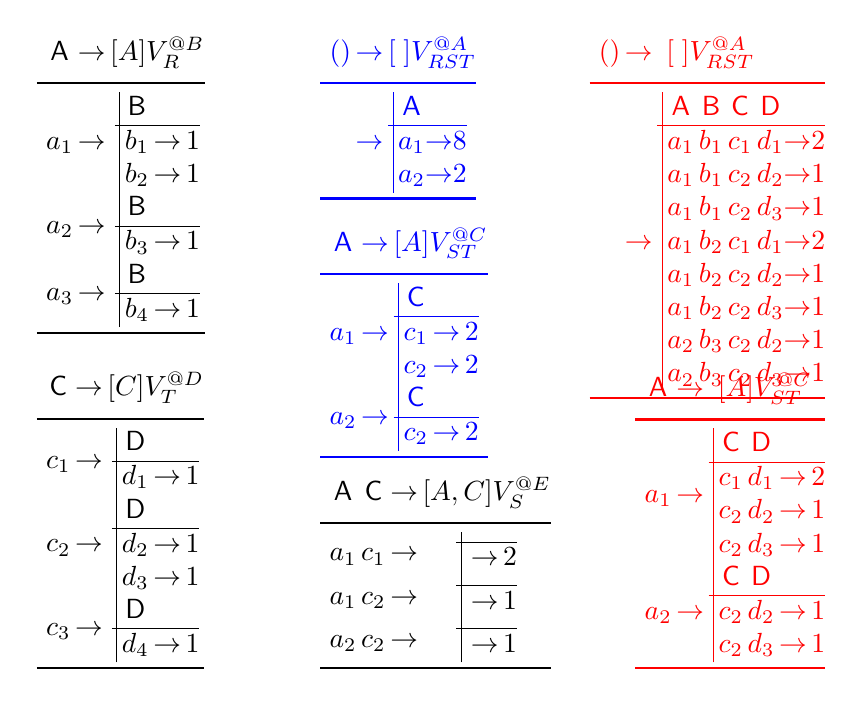
\begin{tikzpicture}[xscale=1.8, yscale=1.01]
  
        % factorized @A
        \node [text=blue, anchor=north west] at (3, 1) {
          \begin{tabular}{@{}l@{\,} @{\,}c@{\,}c@{\,}l@{}}
            & $()$ & $\to$ & $\VIEW[\;]{V^{@A}_{RST}}$ \\[1ex]\toprule 
             & $\tuple{}$ & $\rightarrow$ &
              \begin{tabular}{@{}l@{\,}!{\vrule width 0.03em}@{\,}c@{}c@{}c@{}}
                & $\mathsf{A}$ & & \\
                \specialrule{.03em}{0em}{0em} 
                & $a_1$ & $\rightarrow$ & $8$ \\
                & $a_2$ & $\rightarrow$ & $2$ \\
              \end{tabular}\\\bottomrule 
          \end{tabular}
        };
  
        % flat @A
        \node [text=red, anchor=north east] at (6.7, 1) {
          \begin{tabular}{@{}l@{\,}  @{\,}c@{\,}c@{\,}l@{}}
            & $()$ & $\rightarrow$ & \ $\VIEW[\;]{V^{@A}_{RST}}$ \\[1ex]\toprule
              & $\tuple{}$ & $\rightarrow$ & 
              \begin{tabular}{@{}l@{\,}!{\vrule width 0.03em}@{\,}c@{\,}c@{\,}c@{\,}c@{}c@{}c@{}}
                & $\mathsf{A}$ & $\mathsf{B}$ & $\mathsf{C}$ & $\mathsf{D}$ & & \\
                \specialrule{.03em}{0em}{0em} 
                & $a_1$ & $b_1$ & $c_1$ & $d_1$ & $\rightarrow$ & $2$ \\
                & $a_1$ & $b_1$ & $c_2$ & $d_2$ & $\rightarrow$ & $1$ \\
                & $a_1$ & $b_1$ & $c_2$ & $d_3$ & $\rightarrow$ & $1$ \\
                & $a_1$ & $b_2$ & $c_1$ & $d_1$ & $\rightarrow$ & $2$ \\
                & $a_1$ & $b_2$ & $c_2$ & $d_2$ & $\rightarrow$ & $1$ \\
                & $a_1$ & $b_2$ & $c_2$ & $d_3$ & $\rightarrow$ & $1$ \\
                & $a_2$ & $b_3$ & $c_2$ & $d_2$ & $\rightarrow$ & $1$ \\
                & $a_2$ & $b_3$ & $c_2$ & $d_3$ & $\rightarrow$ & $1$ \\
              \end{tabular}\\\bottomrule
          \end{tabular}
        };
  
        % factorized @C
        \node [text=blue, anchor=north west] at (3, -1.4) {
          \begin{tabular}{@{}l@{\,} @{\,}c@{\,}c@{\,}l@{}}
            & $\mathsf{A}$ & $\rightarrow$ & $\VIEW[A]{V^{@C}_{ST}}$ \\[1ex]\toprule
             & $a_1$ & $\rightarrow$ &
              \begin{tabular}{@{}l@{\,}!{\vrule width 0.03em}@{\,}c@{\,}c@{\,}c@{}}
                & $\mathsf{C}$ & & \\
                \specialrule{.03em}{0em}{0em} 
                & $c_1$ & $\rightarrow$ & $2$ \\
                & $c_2$ & $\rightarrow$ & $2$ \\
              \end{tabular} \\
            \rule{0mm}{4mm} & $a_2$ & $\rightarrow$ &
              \begin{tabular}{@{}l@{\,}!{\vrule width 0.03em}@{\,}c@{\,}c@{\,}c@{}}
                  & $\mathsf{C}$ & & \\
                  \specialrule{.03em}{0em}{0em} 
                  & $c_2$ & $\rightarrow$ & $2$ \\
              \end{tabular}\\\bottomrule 
          \end{tabular}
        };
  
        % flat @C
        \node [text=red, anchor=south east] at (6.7, -7.2) {
          \begin{tabular}{@{}l@{\,} @{\,}c@{\,}c@{\,}l@{}}
            & $\mathsf{A}$ & $\to$ & \ $\VIEW[A]{V^{@C}_{ST}}$ \\[1ex]\toprule
             & $a_1$ & $\rightarrow$ & 
              \begin{tabular}{@{}l@{\,}!{\vrule width 0.03em}@{\,}c@{\,}c@{\,}c@{\,}c@{}}
                & $\mathsf{C}$ & $\mathsf{D}$ & & \\
                \specialrule{.03em}{0em}{0em} 
                & $c_1$ & $d_1$ & $\rightarrow$ & $2$ \\
                & $c_2$ & $d_2$ & $\rightarrow$ & $1$ \\
                & $c_2$ & $d_3$ & $\rightarrow$ & $1$ \\
              \end{tabular}\\
            \rule{0mm}{6mm} & $a_2$ & $\rightarrow$ & 
              \begin{tabular}{@{}l@{\,}!{\vrule width 0.03em}@{\,}c@{\,}c@{\,}c@{\,}c@{}}
                  & $\mathsf{C}$ & $\mathsf{D}$ & & \\
                  \specialrule{.03em}{0em}{0em} 
                  & $c_2$ & $d_2$ & $\rightarrow$ & $1$ \\
                  & $c_2$ & $d_3$ & $\rightarrow$ & $1$ \\
              \end{tabular}\\\bottomrule
          \end{tabular}
        };
  
        % flat/factorized @E
        \node [anchor=south west] at (3, -7.2) {
          \begin{tabular}{@{}l@{\,} @{\,}c@{\,}c@{\,}c@{\,}c@{}}
            %  
            & $\mathsf{A}$ & $\mathsf{C}$ & $\to$ & $\VIEW[A,C]{V^{@E}_{S}}$ \\[1ex]\toprule
             & $a_1$ & $c_1$ & $\rightarrow$ & 
              \begin{tabular}{@{}l@{\,}!{\vrule width 0.03em}@{\,}c@{\,}c@{\,}c@{}}
                & & & \\[-2ex]
                \specialrule{.03em}{0em}{0em} 
                & $\tuple{}$ & $\rightarrow$ & $2$ \\
              \end{tabular} \\
            \rule{0mm}{3mm} & $a_1$ & $c_2$ & $\rightarrow$ & 
              \begin{tabular}{@{}l@{\,}!{\vrule width 0.03em}@{\,}c@{\,}c@{\,}c@{}}
                  & & & \\[-2ex]
                  \specialrule{.03em}{0em}{0em} 
                  & $\tuple{}$ & $\rightarrow$ & $1$ \\
              \end{tabular}\\
            \rule{0mm}{3mm} & $a_2$ & $c_2$ & $\rightarrow$ &
              \begin{tabular}{@{}l@{\,}!{\vrule width 0.03em}@{\,}c@{\,}c@{\,}c@{}}
                  & & & \\[-2ex]
                  \specialrule{.03em}{0em}{0em} 
                  & $\tuple{}$ & $\rightarrow$ & $1$ \\
              \end{tabular}\\\bottomrule
          \end{tabular}
        };
  
        % flat factorized @B
        \node [anchor=north west] at (1, 1) {
          \begin{tabular}{@{}l@{\,} @{\,}c@{\,}c@{\,}c@{}}
            %  
            & $\mathsf{A}$ & $\to$ & $\VIEW[A]{V^{@B}_{R}}$ \\[1ex]\toprule
             & $a_1$ & $\rightarrow$ &
              \begin{tabular}{@{}l@{\,}!{\vrule width 0.03em}@{\,}c@{\,}c@{\,}c@{}}
                & $\mathsf{B}$ & & \\
                \specialrule{.03em}{0em}{0em} 
                & $b_1$ & $\rightarrow$ & $1$ \\
                & $b_2$ & $\rightarrow$ & $1$ \\
              \end{tabular} \\
            \rule{0mm}{4mm} & $a_2$ & $\rightarrow$ &
              \begin{tabular}{@{}l@{\,}!{\vrule width 0.03em}@{\,}c@{\,}c@{\,}c@{}}
                  & $\mathsf{B}$ & & \\
                  \specialrule{.03em}{0em}{0em} 
                  & $b_3$ & $\rightarrow$ & $1$ \\
              \end{tabular} \\
            \rule{0mm}{4mm} & $a_3$ & $\rightarrow$ &
              \begin{tabular}{@{}l@{\,}!{\vrule width 0.03em}@{\,}c@{\,}c@{\,}c@{}}
                  & $\mathsf{B}$ & & \\
                  \specialrule{.03em}{0em}{0em} 
                  & $b_4$ & $\rightarrow$ & $1$ \\
              \end{tabular}\\\bottomrule 
          \end{tabular}
        };
  
        % flat/factorized @D
        \node [anchor=south west] at (1, -7.2) {
          \begin{tabular}{@{}l@{\,} @{\,}c@{\,}c@{\,}c@{}}
            %  
            & $\mathsf{C}$ & $\to$ & $\VIEW[C]{V^{@D}_{T}}$ \\[1ex]\toprule
             & $c_1$ & $\rightarrow$ &
              \begin{tabular}{@{}l@{\,}!{\vrule width 0.03em}@{\,}c@{\,}c@{\,}c@{}}
                  & $\mathsf{D}$ & & \\
                  \specialrule{.03em}{0em}{0em} 
                  & $d_1$ & $\rightarrow$ & $1$ \\
              \end{tabular} \\
            \rule{0mm}{6mm} & $c_2$ & $\rightarrow$ & 
              \begin{tabular}{@{}l@{\,}!{\vrule width 0.03em}@{\,}c@{\,}c@{\,}c@{}}
                & $\mathsf{D}$ & & \\
                \specialrule{.03em}{0em}{0em} 
                & $d_2$ & $\rightarrow$ & $1$ \\
                & $d_3$ & $\rightarrow$ & $1$ \\
              \end{tabular} \\
            \rule{0mm}{4.5mm} & $c_3$ & $\rightarrow$ &
              \begin{tabular}{@{}l@{\,}!{\vrule width 0.03em}@{\,}c@{\,}c@{\,}c@{}}
                  & $\mathsf{D}$ & & \\
                  \specialrule{.03em}{0em}{0em} 
                  & $d_4$ & $\rightarrow$ & $1$ \\
              \end{tabular}\\\bottomrule 
          \end{tabular}
        };
      \end{tikzpicture}
    \end{minipage}
  %}
  \caption{
  Computing the query from Example~\ref{ex:relational_ring} 
  over the database
   in Figure~\ref{fig:count} 
   and the relational ring, where $\forall i\in[12]: p_i=\{ () \to 1 \}$.
   The computation uses 
   the view tree $\tau$
  in Figure~\ref{fig:example_payloads}.
   The red views (rightmost column) have payloads storing the listing representation of the intermediate and final query results. The blue views (top two views in the middle column) encode a factorized representation of these results distributed over their payloads. The remaining (black) views remain the same for both representations.
  }
  \label{fig:factorized_listing_ring}
\end{figure}
  
  

%%%%%%%%%%%%%%%%%%%%%%%%%%%%
We next show how to construct a factorized representation of the query result. In contrast to the scenarios discussed above, this representation is {\em not} available as one payload at the root view, but {\em distributed} over the payloads of all views. This hierarchy of payloads, linked via the keys of the views, becomes the factorized representation. A further difference lies with the multiplication operation. For the listing representation, the multiplication is the Cartesian product. For a given view, it is used to concatenate payloads from its child views. For the factorized representation, we further project away values for all but the marginalized variable. More precisely, for each view $\VIEW[\mathcal{S}]{V^{@X}_{rels}}$ and each of its keys $a_{\mathcal{S}}$, let $\VIEW[\mathcal{T}]{P} = \VIEW[a_\mathcal{S}]{V^{@X}_{rels}}$ be the corresponding payload relation. Then, instead of computing this payload, we compute $\VSUM_{Y\in \mathcal{T}-\{X\}}\VIEW[\mathcal{T}]{P}$ by marginalizing the variables in $\mathcal{T}-\{X\}$ and summing up the multiplicities of the tuples in $\VIEW[\mathcal{T}]{P}$ with the same $X$-value.

\begin{example}
\label{ex:factorized_ring}
We continue Example~\ref{ex:relational_ring}. 
Figure~\ref{fig:factorized_listing_ring} shows the contents of the views with factorized payloads (first two columns in black and blue). 
Each view stores relational payloads that have the schema of the marginalized variable. 
Together, these payloads form a factorized representation over the variable order $\omega$ used to define the view tree in Figure~\ref{fig:example_payloads}. At the top of the factorization, we have a union of two $A$-values: $a_1$ and $a_2$. This is stored in the payloads of (middle) {\color{blue}$\VIEW[\;]{V^{A}_{RST}}$}. The payloads of (middle) {\color{blue}$\VIEW[A]{V^{@C}_{ST}}$} store a union of $C$-values $c_1$ and $c_2$ under $a_1$, and a singleton union of $c_2$ under $a_2$. The payloads of $\VIEW[A]{V^{@B}_R}$ store a union of $B$-values $b_1$ and $b_2$ under $a_1$ and a singleton union of $b_3$ under $a_2$. Note the (conditional) independence of the variables $B$ and $C$ given a value for $A$. This is key to succinctness of factorization. In contrast, the listing representation explicitly materializes all pairings of $B$ and $C$-values for each $A$-value, as shown in the payload of (right) {\color{red}$\VIEW[\;]{V^{A}_{RST}}$}. Furthermore, the variable $D$ is independent of the other variables {\em given} $C$. This is a further source of succinctness in the factorization: Even though $c_2$ occurs under both $a_1$ and $a_2$, the relations under $c_2$, in this case the union of $d_2$ and $d_3$, is only stored once in $\VIEW[C]{V^{@D}_T}$. Each value in the factorization keeps a multiplicity, that is, the number of its derivations from the input data. This is necessary for maintenance. 

This factorization is over a variable order that can be used for all queries with same body and different free variables: As long as their free variables sit on top of the bound variables, the variable order is valid and so is the factorization over it. For instance, if the variable $D$ were not free, then the factorization for the new query would be the same except that we would discard the $D$-values from the payload of the view $\VIEW{V^{@D}_{T}}$.\punto
\end{example}


%%%%%%%%%%%%%%%%%%%%%%%%%%%%

\subsection{Matrix Chain Multiplication}
\label{sec:mcm}

Consider the problem of computing a product of a sequence of matrices $\bm{A}_1, \ldots, \bm{A}_n$ over some ring $\RING$, where matrix $\bm{A}_i[x_i, x_{i+1}]$ has the size $p_{i} \times p_{i+1}$, $i \in [n]$. The product $\bm{A} = \bm{A}_1 \cdots \bm{A}_n$ is a matrix of size $p_1 \times p_{n+1}$ and can be formulated as follows:

\begin{align*}
\bm{A}[x_1, x_{n+1}] = \sum_{x_2 \in[p_2]} \cdots \sum_{x_n\in [p_n]} \prod_{i\in[n]} \bm{A}_i[x_i, x_{i+1}]
\end{align*}

We model a matrix $\bm{A}_i$ as a relation $\VIEW[X_i, X_{i+1}]{A_i}$ with the payload carrying matrix values. The query that computes the matrix $\bm{A}$ is:
\begin{align*}
\VIEW[X_1, X_{n+1}]{A} = \VSUM_{X_2} \cdots \VSUM_{X_n} \VPRODBIG_{i \in [n]} \VIEW[X_i, X_{i+1}]{A_i}
\end{align*}
where each of the lifting functions $\{g_{X_j}\}_{j \in [2,n]}$ maps any key value to payload $\RINGONE\in\RING$.
Different variable orders lead to different evaluation plans for matrix chain multiplication. The optimal variable order corresponds to the optimal sequence of matrix multiplications that minimizes the overall multiplication cost, which is the textbook Matrix Chain Multiplication problem~\cite{Cormen:2009:Algorithms}.

\begin{example}
\label{ex:MCM-factorized-update}
Consider a multiplication chain of $4$ matrices of equal size $p \times p$ encoded as relations $\VIEW[X_i, X_{i+1}]{A_i}$. Let $\mathcal{F} = \{ X_1, X_5 \}$ be the set of free variables and $\omega$ be the variable order $X_1 - X_5 - X_3 - \{ X_2, X_4 \}$, i.e., $X_2$ and $X_4$ are children of $X_3$, with the matrix relations placed below the leaf variables in $\omega$. The view tree $\tau(\omega, \mathcal{F})$ has the following views (from bottom to top; the views at $X_5$ and $X_1$ are equivalent to the view at $X_3$):
\begin{align*}
\VIEW[X_1,X_3]{V^{@X_2}_{A_1A_2}} &= \textstyle\VSUM_{X_2} \VIEW[X_1,X_2]{A_1} \VPROD \VIEW[X_2,X_3]{A_2} \\
\VIEW[X_3,X_5]{V^{@X_4}_{A_3A_4}} &= \textstyle\VSUM_{X_4} \VIEW[X_3,X_4]{A_3} \VPROD \VIEW[X_4,X_5]{A_4} \\
\VIEW[X_1,X_5]{V^{@X_3}_{A_1A_2A_3A_4}} &=\hspace{-0.05em} \textstyle\VSUM_{X_3}\hspace{-0.05em} \VIEW[X_1,X_3]{V^{@X_2}_{A_1A_2}} \hspace{-0.05em}\VPROD\hspace{-0.05em} \VIEW[X_3,X_5]{V^{@X_4}_{A_3A_4}}
\end{align*}
Recomputing these views from scratch for each update to an input matrix takes $\bigO{p^3}$ time. A single-value change in any input matrix causes changes in one row or column of the parent view, and propagating them to compute the final delta view takes $\bigO{p^2}$ time. 
% 
Updates to $\VIEW{A_2}$ and $\VIEW{A_3}$ change every value in $\VIEW{A}$. 
In case of a longer matrix chain, propagating $\VIEW{\delta{A}}$ further requires $\bigO{p^3}$ matrix multiplications, same as recomputation.


We exploit factorization to contain the effect of such changes. For instance, if $\VIEW{\delta{A_2}}$ is a factorizable update  expressible as 
$\VIEW[X_2,X_3]{\delta{A_2}} = \VIEW[X_2]{u} \VPROD \VIEW[X_3]{v}$ (see Section~\ref{sec:factorizable_updates}), then we can propagate deltas more efficiently, as products of 
subexpressions:
\begin{align*}
\quad&\VIEW[X_1,X_3]{\delta{V}^{@X_2}_{A_1A_2}} = \underbrace{\left( \textstyle\VSUM_{X_2} \VIEW[X_1,X_2]{A_1} \VPROD \VIEW[X_2]{u} \right)}_{\VIEW[X_1]{u_2}} \VPROD \VIEW[X_3]{v} \\
&\VIEW[X_1,X_5]{\delta{V}^{@X_3}_{A_1A_2A_3A_4}} = \VIEW[X_1]{u_2} \VPROD \left( \textstyle\VSUM_{X_3} \VIEW[X_3]{v} \VPROD \VIEW[X_3,X_5]{V^{@X_4}_{A_3A_4}} \right)
\end{align*}
Using such factorizable updates enables the incremental computation in $\bigO{p^2}$ time. The final delta is also in factorized form, suitable for further propagation. 

In general, for a chain of $k$ matrices of size $p \times p$, using a binary view tree of the lowest depth, incremental maintenance with factorizable updates takes $\bigO{p^2\log{k}}$ time, while reevaluation takes $\bigO{p^3 k}$ time. The space needed in both cases is $\bigO{p^2 k}$.
\punto
\end{example}

The above example recovers the main idea of LINVIEW~\cite{NEK:SIGMOD:2014}: use factorization in the incremental computation of linear algebra programs where matrix changes are encoded as vector outer products, $\delta{A} = u \TR{v}$. Such rank-$1$ updates can capture many practical update patterns such as perturbations of one complete row or column, or even changes of the whole matrix when the same vector is added to every row or column. \DF generalizes this idea to arbitrary join-aggregate queries. 


% %!TEX root = main.tex

\section{Complexity Analysis}

Consider a query $Q$ over a database $\db$, a set of updatable relations $\mathcal{U}$, and a view tree $\tau$ that corresponds to the query $Q$. 
We analyze the time complexity of processing single-tuple updates to each relation in $\mathcal{U}$ and the space complexity of the materialized views in $\tau$.
We present in section~\ref{ssec:faces} an application of PnP-HVAE on face images, using a pretrained state-of-the-art hierarchical VAE. 
Next, we study the application of our framework to natural images. To that end, we introduce  in section~\ref{ssec:patchVDVAE}  a patch hierachical VAE architecture, that is able to model natural images of different resolutions. In section~\ref{ssec:app_nat}, we provide deblurring, super-resolution and inpainting experiments to demonstrate the relevance of the proposed method.

Additional results are presented in Appendix~\ref{app:add}. All experiments can be reproduced using the code available at \url{https://github.com/jprost76/PnP-HVAE}.



\subsection{Face Image restoration (FFHQ)}\label{ssec:faces}
We first demonstrate the effectiveness of PnP-HVAE on highly structured data, by performing face image restoration.
Latent variable generative models can accurately model structured images such as face images \cite{karras2019style,vahdat2020nvae,child2021very,kingma2018glow}, and then be used to produce high quality restoration of such data. 
In our experiments, we use the VDVAE model of~\cite{child2021very}, pre-trained on the FFHQ dataset~\cite{karras2019style}, as our hierarchical VAE prior.
VDVAE has $L=66$ latent variable groups in its hierarchy and generates images at resolution $256\times256$.

We compare PnP-HVAE with the intermediate layer optimization algorithm (ILO)~\cite{daras2021intermediate} that is based on a different class of generative models than HVAE. ILO is a GAN inversion method which optimizes the image latent code along with the intermediate layer representation of a StyleGAN to generate an image consistent with a degraded observation.
We use the official implementation of ILO, along with a StyleGAN2 model~\cite{karras2020analyzing, stylegan2pytorch}, that was trained for 550k iterations on images of resolution $256\times256$ from FFHQ.  
As VDVAE and StyleGAN models are not trained on the same train-test split of FFHQ, we chose to evaluate the methods on a subset of 100 images from the CelebA dataset~\cite{liu2018large}. 
For super-resolution, the degradation model corresponds to the application of a gaussian low-pass filter followed by a $\times 4$ sub-sampling, and the addition of a gaussian white noise with $\sigma=3$.
For the deblurring, we considered motion blur and  gaussian kernels, both with a noise level $\sigma=8$. %

We provide quantitative comparisons in table~\ref{table:comp_ILO}, along with a visual comparison of the results in figure~\ref{fig:face_restoration}.
PnP-HVAE has the best  PSNR and SSIM results for all the considered restoration tasks, while ILO provides better results  for the perceptual distance.
By jointly optimizing the image and its latent variable, PnP-HVAE provides  results that are both realistic and consistent with the degraded observation.
On the other hand,  ILO  only optimizes on an extended latent space. This method generates  sharp and realistic images with better LPIPS scores,   
but the results lack  of consistency with respect to the observation, which explains the overall lower PSNR performance. 






\subsection{PatchVDVAE: a HVAE for natural images}\label{ssec:patchVDVAE}
Available generative models in the literature operate on images of  fixed resolutions and
are either restrained to datasets of limited diversity, or even to registered face images~\cite{kingma2018glow,child2021very, vahdat2020nvae, karras2019style}, or requiring additional class information~\cite{brock2018large, dhariwal2021diffusion, song2020score, luhman2022optimizing}.
Fitting an unconditional model on natural images appears to be a more difficult task, as their resolution can change, and their content is highly diverse.
The complexity of the problem can be reduced by learning a prior model on patches of reduced dimension. 
For image restoration problems, the patch model can be reused on images of higher dimensions~\cite{zoran2011learning,prost2021learning,altekruger2022patchnr}. When the model is a full CNN, the prior on the set of the  patches can  be computed efficiently by applying the network on the full image~\cite{prost2021learning}.

We thus introduce  patchVDVAE, a fully convolutional hierarchical VAE.
Contrary to existing HVAE models whose resolution is constrained by the constant tensor at the input of the top-down block, patchVDVAE can generate images of different resolutions by controlling the dimension of the input latent. 
This amounts to defining a prior on patches whose dimension corresponds to the receptive field of the VAE. A similar model is used for image denoising in~\cite{prakash2021interpretable}.

 
For PatchVDVAE architecture, we use the same bottom-up and top-down blocks as VDVAE~\cite{child2021very}, and replace the constant trainable input in the first top-down block by a latent variable, to make the model fully convolutional (details on the  architecture are given in Appendix~\ref{app:details}). 
The training dataset is composed of $128\times 128$ patches extracted from a combination of DIV2K~\cite{agustsson2017ntire} and Flickr2K~\cite{Lim_2017_CVPR_workshops} datasets.
We perform data augmentation by extracting  patches at $3$ resolutions: HR-images and $\times 2$ and $\times 4$ downscaled images. 
The model is trained for $7.10^5$ iterations with a batch size of $64$. Following the recommendation of~\cite{hazami2022efficient}, we use Adamax optimizer with an exponential moving average and gradient smoothing of the variance.
We set the decoder model to be a gaussian with diagonal covariance, as in~\cite{luhman2022optimizing}.
PatchVDVAE is fully convolutional and can generate images of dimension that are multiples of $64$ as illustrated by
figure~\ref{fig:vdvae}.

\newlength{\patchwidth}
\setlength{\patchwidth}{0.135\columnwidth}
\begin{figure}[!ht]
    \centering
    \begin{subfigure}[t]{.34\columnwidth}\hspace{0.1cm}
        \setlength{\tabcolsep}{0.02pt}
\renewcommand{\arraystretch}{0}
        \begin{tabular}{*{2}{p{1.03\patchwidth}}}
            \includegraphics[width=\patchwidth]{figures_arxiv/patchVDVAE/samples/generated/64x64/setup-5-image-0018.png} &
            \includegraphics[width=\patchwidth]{figures_arxiv/patchVDVAE/samples/generated/64x64/setup-5-image-0016.png} \\
            \includegraphics[width=\patchwidth]{figures_arxiv/patchVDVAE/samples/generated/64x64/setup-5-image-0008.png} &
            \includegraphics[width=\patchwidth]{figures_arxiv/patchVDVAE/samples/generated/64x64/setup-5-image-0019.png}   
        \end{tabular}
    \end{subfigure}\hspace{-0.15cm}
    \begin{subfigure}[t]{.64\columnwidth}
\begin{tabular}{cc}\vspace{-0.1cm}
\includegraphics[width=2\patchwidth]{figures_arxiv/patchVDVAE/samples/generated/256x256/setup-2-image-0009.png}&
        \includegraphics[width=2\patchwidth]{figures_arxiv/patchVDVAE/samples/generated/256x256/setup-2-image-0002.png}\end{tabular}

    \end{subfigure}
    \caption{\label{fig:vdvae} Left: $64\times64$ patches samples from our patchVDVAE model trained on patches from natural images.
    Right: PatchVDVAE is fully convolutional and it can generate images of higher resolution (here: $128\times128$).\vspace{-0.2cm}}
\end{figure}

\subsection{Natural images restoration}\label{ssec:app_nat}
We  evaluate PnP-HVAE on natural image restoration.
For each task, we report the average value of the PSNR, the SSIM, and the LPIPS metrics on $20$ images from the test set of the BSD dataset~\cite{MartinFTM01}.\\


\noindent
{\bf Image deblurring.}
In the experiments, we consider $2$ gaussian kernels and $2$ motion blur kernels from~\cite{levin2009understanding}, with $3$ different noise levels 
$\sigma \in \{2.55, 7.65, 12.75\}$.
As a baseline we consider  EPLL~\cite{zoran2011learning}, which learns a prior on image patches with a gaussian mixture model.
We also compare PnP-HVAE  with PnP-MMO and GS-PnP, $2$ competing convergent Plug-and-Play methods based on CNN denoisers.
PnP-MMO~\cite{pesquet2021learning} restricts the denoiser to be contraction in order to guarantee the convergence of the PnP forward-backard algorithm. GS-PnP~\cite{hurault2022gradient} considers a gradient step denoiser and reaches state-of-the-art performances of non converging methods~\cite{zhang2021plug}.
We set the temperature $\tau$  in our method as $0.95$, $0.8$ and $0.6$ for noise levels $2.55$, $7.65$ and $12.75$ respectively, and we let it run for a maximum of $50$ iterations. 
For the three compared methods we use the official implementations and pre-trained models provided by the respective authors. 
Details on the choice of hyperparameters for the concurrent methods are provided in the Appendix~\ref{app:details}
Figure~\ref{fig:deblurring_bsd} illustrates that our method provides correct deblurring results. 

According to table~\ref{tab:deb}, the performance of PnP-HVAE is between those of EPLL and GS-PnP and it outperforms PnP-MMO for large noise levels.\\

\begin{table}
\begin{center}\footnotesize
    \begin{tabular}{>{\centering}m{.3cm}*{5}{c}}
    $\sigma$ &Method & PSNR$\uparrow$ & SSIM$\uparrow$ & LPIPS$\downarrow$  \\ 
    \hline
    \multirow{4}{*}{\vcell{$2.55$}}
    & PnP-HVAE & $27.75$ & $0.79$ & $0.31$\\
    & GS-PNP \cite{hurault2022gradient} & $\mathbf{29.59}$ & $\mathbf{0.84}$ & $\mathbf{0.22}$\\
    & EPLL \cite{zoran2011learning} & $26.49$ & $0.71$ & $0.36$\\ 
    & PnP-MMO \cite{pesquet2021learning} & $\underbar{29.50}$ & $\underbar{0.83}$ & $\underbar{0.20}$ \\ \hline
    \multirow{4}{*}{\vcell{$7.65$}}
    & PnP-HVAE & $\underbar{26.36}$ & $\underbar{0.72}$ & $\underbar{0.40}$\\
    & GS-PNP \cite{hurault2022gradient} & $\mathbf{27.33}$ & $\mathbf{0.77}$ & $\mathbf{0.31}$\\
    & EPLL \cite{zoran2011learning} & $24.04$ & $0.66$ & $0.45$ \\ 
    & PnP-MMO \cite{pesquet2021learning} & $25.34$ & $0.69$ & $0.34$\\
    \hline
    \multirow{4}{*}{\vcell{$12.75$}}
    & PnP-HVAE & $\underbar{25.12}$ & $\mathbf{0.73}$ & $\underbar{0.47}$\\
    & GS-PNP \cite{hurault2022gradient} & $\mathbf{26.32}$ & $\mathbf{0.73}$ & $\mathbf{0.37}$\\
    & EPLL \cite{zoran2011learning} & $23.28$ & $0.61$ & $0.51$ \\ 
    & PnP-MMO \cite{pesquet2021learning} & $22.42$ & $0.53$& $0.54$ \\
    \hline
    &\vspace*{-.3cm}\\
            \multicolumn{2}{c}{Blur and motion kernels}& \multicolumn{3}{c}{
        \includegraphics*[scale=1]{figures_arxiv/kernels/4.png}\;\includegraphics*[scale=1]{figures_arxiv/kernels/7.png}\;\includegraphics*[scale=1]{figures_arxiv/kernels/9.png}\;\includegraphics*[scale=1]{figures_arxiv/kernels/11.png}} 
    \end{tabular}
        \caption{\label{tab:deb}Comparison  of PnP-HVAE  and other restoration methods on deblurring. Results are averaged on $4$ kernels.\vspace{-0.2cm}}% on image deblurring.}
    \end{center}
\end{table}

\begin{figure}
    
    \begin{subfigure}[h]{\linewidth}
        \centering
        \includegraphics*[width=\columnwidth]{figures_arxiv/deb_s255_k7.pdf}\vspace{-0.1cm}
        \caption{Gaussian blur, $\sigma=2.55$}
    \end{subfigure}
    \begin{subfigure}[h]{\linewidth}
        \centering
        \includegraphics*[width=\columnwidth]{figures_arxiv/deb_s765_k11.pdf}\vspace{-0.1cm}
        \caption{Motion blur, $\sigma=7.65$}
    \end{subfigure}\vspace*{-0.1cm}
    \caption{\label{fig:deblurring_bsd} Natural image deblurring\vspace{-0.1cm}}
\end{figure}

\noindent {\bf Effect of the temperature.}
PnP-HVAE gives control on the temperature of the prior over the latent space.
In figure~\ref{fig:temp_effect}, we illustrate that reducing the temperature increases the strength of the regularization prior. In this example the tuning $\tau=0.7$ produces the best performance.\\
\begin{figure}[!ht]
   
    \includegraphics[width=\columnwidth]{figures_arxiv/demo_temp.pdf}\vspace{-0.15cm}
    \caption{ \label{fig:temp_effect} Effect of the temperature in PnP-VAE on a deblurring problem, with $\sigma=7.65$.\vspace{-0.15cm}}
\end{figure}


\noindent
{\bf Image inpainting.}
Next we consider the task of noisy image inpainting. 
We compose a test-set of 10 images from the validation set of BSD~\cite{MartinFTM01} and we create masks
  by occluding diverse objects of small size in the images. 
A gaussian white noise with $\sigma=3$ is added to the images.
As a comparaison, we still consider GS-PnP and EPLL.
For PnP-HVAE, the temperature is set to $\tau=0.6$, and the algorithm is run for a maximum of $200$ iterations, unless the residual $||\x_{k+1}-\x_k||$ is on a plateau.
We provide on Table~\ref{tab:inpainting_bsd} the distortion metrics with the ground truth, as well as a visual
\begin{table}



\begin{center}
    \begin{tabular}{cccc}
        & PSNR$\uparrow$ & SSIM$\uparrow$ &LPIPS$\downarrow$ \\\hline
        PnP-HVAE  & $\mathbf{29.54}$ & $\mathbf{0.93}$ & $\mathbf{0.06}$\\
        GS-PNP & $28.52$ & $\mathbf{0.93}$ & $0.09$\\
        EPLL & $\underline{29.16}$ & $\mathbf{0.93}$ & $\mathbf{0.06}$\\
    \end{tabular}
    \caption{\label{tab:inpainting_bsd}Quantitative evaluation for inpainting on BSD.}
    \end{center}
\end{table}
comparison on figure~\ref{fig:inpainting_bsd}. 
With its hierarchical structure,  PnP-HVAE outperforms the compared methods. \vspace{0.05cm}



\begin{figure}[!h]
    \includegraphics[width=\columnwidth]{figures_arxiv/demo_inp_bsd2.pdf}\vspace{-0.1cm}
    \caption{\label{fig:inpainting_bsd}Natural image inpainting\vspace{-0.3cm}}
\end{figure}











\section{Related work}
\noindent \textbf{Video foundation models.}
With sufficient computational power and an abundant source of data, there have been attempts to build a single large-scale foundation model that can be adapted to diverse downstream tasks.
Along with the success of foundations models in the natural language processing domain~\cite{brown2020language,chen2021evaluating,devlin2019bert} and in computer vision~\cite{bertasius2021space,jia2021scaling,radford2021learning}, video data has become another data type of interest, as it has grown in scale due to numerous internet video-sharing platforms.
Accordingly, several methods to train a video foundation model have been proposed.
Due to the innate multi-modality of video data, \textit{i.e.}, a combination of visual $\cdot$ vocal $\cdot$ textual context, most works have centered around the variations of the cross-modal attention mechanism \cite{akbari2021vatt,bertasius2021space,gabeur2020multi,luo2020univl,neimark2021video,tan2021look,wei2020multi,yang2021taco}.
In addition, as most video data lack proper labels or descriptions, contrastive learning methods were studied to learn meaningful feature representations or enhance video-text alignment in a self-supervised manner \cite{akbari2021vatt,kuang2021video,luo2020univl,yang2021taco}.

More specifically, MERLOT \cite{zellers2021merlot} proposed a multi-modal representation learning method for visual commonsense reasoning, which also performed well in twelve video reasoning tasks.
VATT \cite{akbari2021vatt} introduced a multi-modal learning method via contrastive learning. 
The pre-trained model performed well in a variety of vision tasks from image classification to video action recognition and zero-shot video retrieval.
Another representative work, UniVL \cite{luo2020univl} proposed a straightforward pre-training method with auxiliary loss functions. 
After fine-tuning on a specific task, the pre-trained model performed outstandingly in a wide range of tasks of text-to-video retrieval, action segmentation, action step localization, video sentiment analysis, and video captioning.
Other foundation models for multiple video tasks include \cite{li2020hero,sun2019learning,sun2019videobert,zhu2020actbert,fu2021violet,wang2022all}. 

\noindent \textbf{Auxiliary learning.}
In order to enhance the performance of one or a multitude of primary tasks, auxiliary learning methods can be incorporated.
\cite{ruder2017overview} introduced Multi-task learning (MTL) to the deep neural networks by training a single model with multiple task losses to assist learning on the main task.
Such a method is generally adapted to pre-train the foundation models in the self-supervised manner~\cite{li2020hero,sun2019learning,sun2019videobert,zhu2020actbert,fu2021violet,wang2022all}.
However, these various pretext task losses used in the pre-training phase are ignored in the fine-tuning phase, and only the primary task loss is minimized.

Recently, meta-learning methods have been introduced for auxiliary learning.
\cite{liu2019self,navon2020auxiliary,shu2019meta} proposed a meta-learning method in which the model learns auxiliary tasks to generalize well to unseen data. 
In these settings, a separate subset of data is held out as the primary task, while the others are used as auxiliary tasks that aid the primary task's performance.
Similar methods were adopted for computer vision tasks such as semantic segmentation \cite{xu2021leveraging}.
Other domain applications include navigation tasks with reinforcement learning \cite{ye2021auxiliary}, or self-supervised learning methods on graph data \cite{hwang2020self}.
\section{Conclusion}\label{sec:conclusion}
In this work, we focus on addressing the fundamental challenge of OOD detection tasks, which is how to fully understand the semantic discrepancy between the ID/OOD samples. We reveal that the key to success in the realistic SCOOD task is to allocate as many ID samples in the unlabeled set correctly as possible. To this end, we propose a novel uncertainty-aware optimal transport scheme that introduces class-specific energy scores as guidance for effective label assignment. Experimental results show that our method achieves better performance than previous state-of-the-art methods on SCOOD benchmarks.

\textbf{Limitations.} In addition to temperature scaling, other techniques such as feature clipping applied in ReAct~\cite{sun2021react} also enhance the performance of energy score, so how to obtain an OOD score that best fits the SCOOD task can be further explored. Moreover, a setting highly related to SCOOD has been proposed in \cite{katz2022training} and formulated as a constrained optimization problem. We will also theoretically analyze these practical OOD settings in our feature work.

% \section*{Acknowledgments}
\textbf{Acknowledgments.} 
This work is supported by National Key R\&D Program of China under Grant 2020AAA0105701, National Natural Science Foundation of China (NSFC) under Grants 61872327, Major Special Science and Technology Project of Anhui, National Natural Science Foundation of China (62033012) and Ant Group through Ant Research Intern Program.

%\section{Note on Complexity of \DF}
\label{appendix:complexity}

Due to lack of space, we only mention the complexity of \DF without proof. Let $Q$ be the conjunctive query, $\omega$ its variable order, $\tau$ the view tree modeled on $\omega$, and $\mathcal{D}$ the database of input {\color{blue}relations}. Let $N$ be the maximum size of a {\color{blue}relation} in $\mathcal{D}$. We next assume view trees with indicator projections as introduced in Appendix~\ref{sec:cyclic_queries}.

{\bf Computation.} The time to compute the keys of any view in the view tree $\tau$ is $O(N^{{\it fhtw}(\omega)})$, where $\mathit{fhtw}(\omega)$ is the fractional hypertree width of the variable order $\omega$~\cite{Olteanu:FactBounds:2015:TODS,FAQ:PODS:2016}. By taking the variable order that minimizes ${\it fhtw}(\omega)$, we obtain the fractional hypertree width ${\it fhtw}(Q)$ of $Q$~\cite{Marx:2010}.

The above analysis ignores payload computation! For the standard sum-product ring (e.g., $\mathbb{R}$), the additional complexity brought by payload computation is subsumed by the above upper bound. For the degree-$m$ matrix ring, the additional complexity factor is $O(m^2)$, totalling $O(N^{{\it fhtw}(\omega)}\cdot m^2)$. However, for the relational data ring, the payload size may become larger than the key size. Assuming a worst-case optimal join algorithm for computing the cyclic joins, e.g., LeapFrog TrieJoin~\cite{Veldhuizen14:LFTJ}, the time to compute the payloads is $O(N^{\rho^*(Q)})$, where $\rho^*(Q)$ is the fractional edge cover number of $Q$~\cite{AGM:2013}. For payloads encoding the factorized representation of the result of $Q$, the overall complexity remains $O(N^{{\it fhtw}(\omega)})$ since the cumulative size of all payloads of the views in the view tree is  $O(N^{{\it fhtw}(\omega)})$.

{\bf Maintenance.} The previous complexity results are for computation from scratch. We next discuss the complexity for maintenance under single-tuple update to some of the input {\color{blue}relations}. The complexity may become lower since the variables that appear in the updated {\color{blue}relations} are fixed to the constants in the update. Let $Q_u$ be the query $Q$ where all variables fixed to constants by the updates are removed; if a {\color{blue}relation} has no variable left, then it is removed from $Q_u$. Then, we define the {\em dynamic fractional hypertree width} of $Q$ as the fractional hypertree width of $Q_u$: $\mathit{dfhtw}(Q) = \mathit{fhtw}(Q_u)$. Similarly, the {\em dynamic fractional edge cover number} of $Q$ is the fractional edge cover number of $Q_u$: $\mathit{d\rho^*}(Q) = \mathit{\rho^*}(Q_u)$. Then, all complexity results from the previous computation case hold for maintenance where we replace the widths by their dynamic counterparts.







\bibliographystyle{abbrv}
\bibliography{bibliography}

\end{document}
